\documentclass[12pt,twoside,a4]{article}
\usepackage{subfiles}
%DIZIONARIO E FONT
\usepackage[T1]{fontenc}
\usepackage[utf8x]{inputenc}
\usepackage[italian]{babel}
\usepackage{lmodern}

%TITOLO
\author{\strut}
\date{\strut}
\makeatletter
\renewcommand\maketitle[1][]{
{\raggedright
\begin{center}
\Huge \textit{\textbf{\@title}}\\[1.5ex]
\Large \@author \\[1.5ex]
\large \@date \\[1.5ex]
\end{center}
\ifstrequal{#1}{toc=off}{\bigskip}
{\ifstrequal{#1}{toc=on}{ \vspace*{\fill} \tableofcontents \vspace*{\fill}\thispagestyle{empty}  \newpage}{}} \pagenumbering{arabic}
}}
\makeatother

%GEOMETRIA
\usepackage[left=2.5cm, right=2.5cm, top=2.5cm, bottom=2.5cm, includefoot, headheight=13.6pt]{geometry}

%HYPERLINKS
\usepackage[colorlinks = true,
linkcolor = black,
urlcolor  = blue,
citecolor = black,
anchorcolor = black
]{hyperref}

%LINGUAGGIO MATEMATICO
\usepackage{amssymb, amsmath, latexsym}
\usepackage{physics}
\usepackage{bbold}
\usepackage{nccmath}
\usepackage[makeroom]{cancel}
\renewcommand{\Hat}[1]{\boldsymbol{\hat{\mathbf{#1}}}}
\renewcommand{\vec}{\textbf}
\DeclareUnicodeCharacter{2032}{\textendash} %apostrofo in math mode
\everymath{\displaystyle}

%GRAFICA
\usepackage{graphicx}
\usepackage{mdframed}
\usepackage{float}

%COMANDI DI STRUTTURA
\usepackage{caption}
\usepackage{xcolor}
\usepackage{enumitem}
\usepackage{changepage}
\usepackage{etoolbox}
\usepackage{titlesec}
\usepackage{comment}
\usepackage{marginnote}
\usepackage{footnotehyper}
\usepackage[bottom]{footmisc}
\renewcommand*{\marginfont}{\footnotesize\itshape}

%INIDICE E TITOLI
\usepackage{tocloft}
\addto\captionsitalian{\renewcommand{\contentsname}{\LARGE \hspace{-3pt}Contenuti}}
\renewcommand{\cftsubsecfont}{\normalfont}
\renewcommand{\cftsecfont}{\large \bfseries }
\titleclass{\subsubsubsection}{straight}[\subsection]

\newcounter{subsubsubsection}[subsubsection]
\renewcommand\thesubsubsubsection{\thesubsubsection.\arabic{subsubsubsection}}
\renewcommand\theparagraph{\thesubsubsubsection.\arabic{paragraph}} % optional; useful if paragraphs are to be numbered
\titleformat{\subsubsubsection}
  {\normalfont\normalsize\bfseries}{\thesubsubsubsection}{1em}{}
\titlespacing*{\subsubsubsection}
{0pt}{3.25ex plus 1ex minus .2ex}{1.5ex plus .2ex}
\makeatletter
\renewcommand\paragraph{\@startsection{paragraph}{5}{\z@}%
  {3.25ex \@plus1ex \@minus.2ex}%
  {-1em}%
  {\normalfont\normalsize\bfseries}}
\renewcommand\subparagraph{\@startsection{subparagraph}{6}{\parindent}%
  {3.25ex \@plus1ex \@minus .2ex}%
  {-1em}%
  {\normalfont\normalsize\bfseries}}
\def\toclevel@subsubsubsection{4}
\def\toclevel@paragraph{5}
\def\toclevel@paragraph{6}
\def\l@subsubsubsection{\@dottedtocline{4}{7em}{4em}}
\def\l@paragraph{\@dottedtocline{5}{10em}{5em}}
\def\l@subparagraph{\@dottedtocline{6}{14em}{6em}}
\makeatother
\setcounter{secnumdepth}{4}
\setcounter{tocdepth}{4}
\titleformat{\section}
{\Huge\bfseries}{\thesection}{1em}{}
\titleformat{\subsection}
{\Large\bfseries}{\thesubsection}{1em}{}
\titleformat{\subsubsection}
{\large\bfseries}{\thesubsubsection}{1em}{}

%TEOREMI
\usepackage{amsthm}
\newtheoremstyle{a capo}% nome dello stile
  {\topsep}% spazio sopra
  {\topsep}% spazio sotto
  {\itshape}% font del corpo
  {}% indentazione del primo paragrafo
  {\bfseries}% font dell'intestazione
  {}% punteggiatura dopo l'intestazione
  {\newline}% spazio dopo l'intestazione
  {\thmname{#1}\thmnumber{ #2}\thmnote{ (#3)}}% formato dell'intestazione
 \newtheoremstyle{due punti}% nome dello stile
  {\topsep}% spazio sopra
  {\topsep}% spazio sotto
  {\itshape}% font del corpo
  {}% indentazione del primo paragrafo
  {\bfseries}% font dell'intestazione
  {:}% punteggiatura dopo l'intestazione
  { }% spazio dopo l'intestazione
  {\thmname{#1}\thmnumber{ #2}\thmnote{ (#3)}}% formato dell'intestazione
  
\newtheorem{pro}{Proposizione}
\newtheorem{cor}{Corollario}

\theoremstyle{due punti}
\newtheorem{df}{Definizione}
\theoremstyle{a capo}
\newtheorem{teo}{Teorema}
\newtheorem{pr}{Principio}
\newcommand\oss{\noindent \textbf{Osservazione: }}

%CONTATORI
\usepackage{chngcntr}
\usepackage{alphalph}
\renewcommand{\thesubsection}{\arabic{subsection}}
\counterwithin{df}{subsection}
\counterwithin*{pr}{subsection}
\counterwithin{pro}{subsection}
\counterwithin{cor}{subsection}
\counterwithin{teo}{subsection}
\newcounter{es}
\counterwithin*{es}{section}
\newcounter{ese}
\counterwithin*{ese}{subsection}
\counterwithin{equation}{subsection}
\newcounter{aa}
\setcounter{aa}{\the\year}
\addtocounter{aa}{-1}

%DERIVATE E COMANDI MATEMATICI
\newenvironment{pp}[2]{\frac{\partial #1}{\partial #2}}{}
\renewenvironment{dd}[2]{\frac{d #1}{d #2}}{}
\renewcommand{\parallel}{\mathrel{/\mkern-5mu/}}
\makeatletter
\newcommand{\notparallel}{
  \mathrel{\mathpalette\not@parallel\relax}}
\newcommand{\not@parallel}[2]{
  \ooalign{\reflectbox{$\m@th#1\smallsetminus$}\cr\hfil$\m@th#1\parallel$\cr}}
\newcommand{\longmatrix}[4]{\left( \begin{matrix}     #1 & \dots  & #2\\ \vdots & \ddots & \vdots\\ #3 & \dots  & #4 \end{matrix} \right)}
\newcommand{\vettore}[1]{\left( \begin{array}{c} #1 \end{array} \right)}

%AMBIENTI

\newcommand{\theindexsol}{$\R$}
\newcounter{solution}
\setcounter{solution}{0}
\counterwithin{solution}{subsection}
\newenvironment{solution}[1][]{
  \stepcounter{solution} 
  \medskip 
  \noindent\fbox{\textbf{Soluzione~\theindexsol-\thesolution}}\hrulefill\par\vspace{10pt}\noindent\rmfamily%
    \label{sol:\thesolution}%
    \noindent}{
	\medskip
    \par\noindent\hrulefill%
    \fbox{\textbf{Esercizio a pagina: \pageref{es:\thesolution}}}\par\vspace{10pt}% 
}

\newcounter{esercizio}
\setcounter{esercizio}{0}
\counterwithin{esercizio}{subsection}
\newcommand{\theindexese}{$\R$}
\newenvironment{esercizio}[2][]{
  \stepcounter{esercizio} 
  \newcommand{\pagesol}{\pageref{sol:\theesercizio}}
  \medskip 
  \noindent\fbox{\bfseries{Esercizio~\theindexese-\theesercizio~\textit{#1}}}\hrulefill\par\vspace{10pt}\noindent\rmfamily%
    \label{es:\theesercizio}%
    \noindent }{ 
	\medskip
    \par\noindent\hrulefill%
    \ifcsname r@sol:\theesercizio\endcsname
      \fbox{\textbf{Soluzione a pagina: \pageref{sol:\theesercizio}}}\par\vspace{10pt}% 
    \else
      \fbox{\textbf{Chi fa da sé, fa per tre}}\par\vspace{10pt}% 
    \fi
}




%DIMOSTRAZIONE
\newenvironment{dm}[1][] {\medskip \begin{adjustwidth}{1cm}{} \begin{mdframed}[linewidth=1.5,linecolor=gray, topline=false,rightline=false,bottomline=false] \textbf{ Dimostrazione:}{ \itshape #1\ }}{\medskip \hfill{$\square$} \end{mdframed}\end{adjustwidth} \bigskip}
%ESEMPIO
\definecolor{gialloverde}{RGB}{112, 177, 63}
\newenvironment{esempio}[1][] {\medskip \begin{adjustwidth}{1cm}{} \begin{mdframed}[linewidth=1.5,linecolor=gialloverde, topline=false,rightline=false,bottomline=false] \textcolor{gialloverde}{\textbf{Esempio{: #1} \newline}}}{\medskip\end{mdframed}\end{adjustwidth} }

%OSSERVAZIONE
\newlist{osservazioneenum}{enumerate}{1}
\setlist[osservazioneenum]{label=(\textit{\roman*})\hspace{0.5em}, leftmargin=0pt, labelsep=0pt, itemindent=2em}

\newenvironment{osservazioni}[1][]{
  \medskip
  \begin{adjustwidth}{1cm}{}
    \textbf{\textit{Osservazioni:}}\newline
    \vspace{-0.5cm}
    \begin{osservazioneenum}[label=(\textit{\roman*})\hspace{0.5em}, leftmargin=0pt, labelsep=0pt, itemindent=2em]}{
    \end{osservazioneenum}
  \end{adjustwidth}}
  
\newenvironment{osservazione}[1][]{
  \bigskip
  \begin{adjustwidth}{1cm}{}
    \textbf{\textit{Osservazione:}}\vspace{0.1cm} \newline}{
  \everypar{\leftskip=0pt} % Ripristina il rientro del testo
  \end{adjustwidth}}

%IMPAGINAZIONE
\usepackage{fancyhdr}% http://ctan.org/pkg/fancyhdr
\fancypagestyle{thesis}{%
\fancyhf{}
\renewcommand{\headrulewidth}{0.4pt}
\fancyhead[ER]{\textbf{\leftmark}}
\fancyhead[OL]{\textbf{\rightmark}}
\fancyfoot[LO,RE]{\thepage}}

\usepackage{ifthen}
\let\originalsection\section
\renewcommand{\section}[2][]{%
  \ifthenelse{\equal{#1}{}}%
    {\stepcounter{section} \originalsection*{#2}%
     \addcontentsline{toc}{section}{#2}}%
    { %
     \addcontentsline{toc}{section}{#1}}%
       \ifstrempty{#1}
    {\markboth{\MakeUppercase{#2}}{\rightmark}}%
    {\markboth{#1}{\rightmark}}%
}

\let\originalsubsection\subsection
\renewcommand{\subsection}[2][]{%
  \ifstrempty{#1}
    {\originalsubsection{#2}
     \markright{\thesubsection. #2}}%
    {\originalsubsection[#1]{#2}
     \markright{\thesubsection. #1}}%
}

%ADDARI LESSICO

\newcommand{\gras}[1]{\textbf{#1}}
\newcommand{\vet}[1]{\vec{#1}}
\newcommand{\ps}[2]{\langle{#1},{#2}\rangle}
\newcommand{\norma}[1]{\| #1 \|}


\newcommand{\duno}[2]{\frac{\partial{#1}}{\partial{#2}}}
\newcommand{\Duno}[2]{\dfrac{\partial{#1}}{\partial{#2}}}
\newcommand{\deuno}[2]{{\partial}_{#2} {#1}}
\newcommand{\dtot}[2]{\dfrac{\mbox{d}{#1}}{\mbox{d}{#2}}}

\newcommand{\ddue}[2]{\frac{\partial^2{#1}}{\partial{{#2}^2}}}
\newcommand{\Ddue}[2]{\dfrac{\partial^2{#1}}{\partial{{#2}^2}}}
\newcommand{\dedue}[2]{{{\partial}^2}_{#2} {#1}}
\newcommand{\ddtot}[2]{\dfrac{\mbox{d}^2 {#1}}{\mbox{d}{#2}^2}}




\newcommand{\soprau}[1]{\stackrel{\mathclap{\normalfont\mbox{#1}}}{=}}
\newcommand{\spazio}{\hspace{0.25em}}
\newcommand{\pippo}{\hspace{0.5em}}
\newcommand{\SP}{\mbox{ }}
\newcommand{\modulo}[1]{\left| {#1} \right|}
\newcommand{\quadre}[1]{\left[ {#1} \right]}
\newcommand{\graffe}[1]{\lbrace {#1} \rbrace}
\newcommand{\tonde}[1]{\left({#1}\right)}
\newcommand{\uncini}[1]{\langle #1 \rangle}
\newcommand{\wt}[1]{\widetilde{#1}}
\newcommand{\wh}[1]{\widehat{#1}}



%ALFABETO MATEMATICO
\newcommand{\A}{\mathcal{A}}
\newcommand{\B}{\mathcal{B}}
\newcommand{\C}{\mathcal{C}}
\newcommand{\Cc}{\mathbb{C}}
\newcommand{\D}{\mathcal{D}}
\newcommand{\E}{\mathcal{E}}
\newcommand{\F}{\mathcal{F}}
\newcommand{\G}{\mathcal{G}}
\renewcommand{\H}{\mathcal{H}}
\newcommand{\I}{\mathcal{I}}
\renewcommand{\L}{\mathcal{L}}
\newcommand{\M}{\mathcal{M}}
\newcommand{\N}{\mathcal{N}}
\renewcommand{\O}{\mathcal{O}}
\renewcommand{\P}{\mathcal{P}}
\newcommand{\Q}{\mathcal{Q}}
\newcommand{\R}{\mathcal{R}}
\newcommand{\Rr}{\mathbb{R}}
\renewcommand{\S}{\mathcal{S}}
\newcommand{\T}{\mathcal{T}}
\newcommand{\U}{\mathcal{U}}
\newcommand{\V}{\mathcal{V}}
\newcommand{\W}{\mathcal{W}}
\newcommand{\X}{\mathcal{X}}
\newcommand{\Y}{\mathcal{Y}}
\newcommand{\Z}{\mathcal{Z}}
\newcommand{\1}{\mathbb{1}}
\newcommand{\mev}{\mathrm{MeV}}


\DeclareMathOperator{\arcsinh}{arcsinh}
\DeclareMathOperator{\arctg}{arctg}
\DeclareMathOperator{\tg}{tg}


\begin{document}
\setlength{\headheight}{15.2pt}

\title{Raccolta di esercizi di \\Fisica Moderna}
\author{Diletta Viola \\ \small{\href{mailto:\\ diletta.viola@studenti.unipd.it}{diletta.viola@studenti.unipd.it}}\\ \Large Pietro Scapolo \\ \small{\href{mailto:\\ pietro.scapolo@studenti.unipd.it}{pietro.scapolo@studenti.unipd.it}}}
\maketitle[toc=off]
\pagestyle{empty}
\vspace*{\fill} 
\begin{center}
    \textit{\textbf{ \Huge Prefazione}}
\end{center}
    \begin{adjustwidth}{0.15\textwidth}{0.15\textwidth}
    \begin{center}
    Questo documento contiene una raccolta di esercizi risolti relativi al corso di Fisica Moderna tenuto dai Professori F. Seno e S. Rigolin presso il Dipartimento di Fisica e Astronomia ”Galileo Galilei” dell'Università degli Studi di Padova. Le soluzioni riportate non sono state revisionate dai Professori, i quali non hanno alcuna responsabilità sul contenuto e pertanto non escludiamo che ci possano essere degli errori. Gli esercizi sono principalmente tratti dai file disponibili sul Moodle dei corsi che i Professori stessi hanno condiviso e che, in alcuni casi, hanno svolto in aula durante le lezioni. 
    Concludiamo sottolineando che questo lavoro nasce dalla necessità di avere a disposizione un manuale di esercizi per prepararsi all'esame poiché non esistono altre raccolte disponibili.
    Se trovate eventuali errori segnalateceli via mail!
    \end{center}
    \end{adjustwidth}


\setcounter{tocdepth}{2}

\vspace*{\fill} 
\pagestyle{empty}
\pagenumbering{none}
\vspace*{\fill}
\tableofcontents 
\vspace*{\fill}


\pagestyle{thesis}
\pagenumbering{arabic}\markboth{RELATIVITÀ}{1 Cinematica relativistica}
\section{Relatività }
\subsection{Cinematica relativistica}

\begin{esercizio}
	-Due razzi A e B, ciascuno avente una lunghezza propria $l_0 = 100$m, si incrociano, scorrendo parallelamente uno all'altro, venendo da direzioni oiooste. Secondo l'orologio del razzo A, la testa di B ci mette un tempo $t = 1.5 \cdot 10^{-6}$ s per passare l'intera lunghezza di A.
	\begin{enumerate}[label=(\textit{\roman*})]
		\item Quale è la velocità  relativa dei razzi?
		\item Secondo gli orologi del razzo B, quanto ci mette la testa di A a passare l'intera lunghezza di B?
		\item Secondo gli orologi di B quanto tempo passa tra quando la testa A passa la testa di B e la coda di A passa la testa di B? Come si concilia questa risposta con quella precedente?
	\end{enumerate}
\end{esercizio}

\begin{esercizio}
	-Le coordinate spazio temporali di due eventi, misurati in un sistema di riferimento inerziale S, sono $(x_1=L, \ t_1 = \frac{L}{c})$ e $(x_2=2L,\  t_2 = \frac{L}{2c})$. Trovare la velocità  del sistema di riferimento S' nel quale i due eventi avvengono simultaneamente e calcolare quanto vale questo tempo.
\end{esercizio}

\begin{esercizio}
	-Un sistema di riferimento inerziale S' si muove lungo l'asse x di un sistema di riferimento S a velocità  $v$. Nel sistema S una sbarra lunga $1$m parallela all'asse x si muove verso l'alto (direzione y) con velocità  $u$. Il centro della sbarra passa per il punto $x=y=x^\prime =y^\prime =0$ a $t=t' =0.$
	\begin{enumerate}[label=(\textit{\roman*})]
		\item Arguire, usando solo il concetto di relatività  della simultaneità  e senza fare calcoli, che la sbarra è piegata verso l'alto nel sistema S'
		\item Calcolare l'angolo $\theta ^\prime$ di questo piegamento.
	\end{enumerate}
\end{esercizio}

\newpage
\begin{esercizio}
	-Un sistema di riferimento S' ha velocità $v=0.6c$ \ rispetto ad S. A $t' = 10^{-7} $ \ s una particella lascia il punto $x'= 12$ \ m viaggiando nella direzione negativa con una velocità $u'= - \frac{c}{3}$ \ . La particella si ferma improvvisamente a $t'=3\cdot 10^{-7}$ \ s 
\begin{enumerate}[label=(\textit{\roman*})]
		\item Qual è la velocità della particella nel sistema S?
		\item Di quanto si è spostata la particella nel sistema S?
	\end{enumerate}
 
\end{esercizio}


\begin{esercizio}
	-Un osservatore inerziale S vedi i corpi A e B muoversi con velocità  $v_{\mathrm{A}}=\frac{4}{5}c$ \ e \ $v_{\mathrm{B}}=\frac{3}{5}c$ lungo l'asse $x$. Sapendo che un corpo C, che si muove sempre lungo x, vede sia A che B muoversi verso di lui con una velocità  in modulo uguale, determinare la velocità  di C nel sistema S.
\end{esercizio}

\begin{esercizio}
	-Un segnale luminoso viene emesso ad un angolo $\theta '$ da un sistema inerziale S′ che si muove lungo l'asse x di un sistema S. Se ( $c \cos \theta', c \sin \theta '$) sono le componenti del segnale in S′, determinare le componenti nel sistema S.
\end{esercizio}

\begin{esercizio}
	-In un sistema di riferimento inerziale S due corpi 1 e 2 partono contemporaneamente dall'origine O con velocità  $v_1=-v_2=v=\frac{3}{5}c$. Determinare la distanza tra i due corpi nel sistema S e nel sistema S′, solidale al corpo 1, quando il corpo 1 arriva al punto A di coordinata L in S.
\end{esercizio}

\begin{esercizio}
	-In un sistema di riferimento inerziale vengono registrati due eventi di coordinate
	\begin{gather*} 
		ct_1=0 , x_1=0, y_1=0, z_1=0 \\
		ct_2=0 , x_2=0, y_2=0, z_2=0 
	\end{gather*}
	Determinare un sistema di riferimento S′ in cui i due eventi siano simultanei.
\end{esercizio}

\begin{esercizio}
	-In un sistema di riferimento inerziale S ci stiamo avvicinando con velocità  costante ad uno specchio fisso. Inviamo un segnale luminoso in direzione perpendicolare allo specchio con frequenza $\nu = 10^9$ Hz. Dopo 2 sec riceviamo il segnale riflesso ad una frequenza $\nu'=1,32 \cdot 10^9$ Hz. Quanto tempo passa dall'invio del segnale al momento in cui noi impattiamo sullo specchio?
\end{esercizio}

\newpage
\subsection{Dinamica relativistica}

\begin{esercizio}
	-La nostra galassia si estende approssimativamente per $10^5$ anni luce e un protone ha approssimativamente una energia di $10^{19}$ \ eV. Per quanto tempo dovrebbe viaggiare con questa energia per attraversare la galassia, nel sistema di riferimento della galassia? E nel suo sistema di riferimento?
\end{esercizio}

\begin{esercizio}
	-Graficare la energia totale in funzione del momento per una particella di massa $m_0$ per i casi:
	\begin{enumerate}[label=(\textit{\roman*})]
		\item Dinamica Newtoniana;
		\item Dinamica Relativistica;
		\item Dinamica Relativistica per particella di massa nulla.
	\end{enumerate}
\end{esercizio}

\begin{esercizio}
	-Un elettrone è accelerato da fermo da un potenziale di $10^5$ V e poi procede a velocità  costante.
	\begin{enumerate}[label=(\textit{\roman*})]
		\item Quanto tempo ci mette l'elettrone a percorrere 10 m dopo che ha raggiunto la sua velocità  finale?
		\item Qual è la distanza misurata nel sistema di riferimento dell'elettrone?
	\end{enumerate}
\end{esercizio}


\begin{esercizio}
-Una navicella spaziale si muove nello spazio libero attraverso la propulsione fornita da un laser stazionario proveniente dalla terra. Se la navicella è perfettamente riflettente, calcolare la massa equivalente di luce richiesta per accelerare il veicolo di massa a riposo $m_0$ fino ad un fissato $\gamma$.
\end{esercizio}

\newpage
\begin{esercizio}
	-Una particella ha una energia cinetica uguale a due volte la sua massa. Trovare la sua velocità  ed il suo momento. Come cambiano questi risultati se l'energia  è cinque volte la massa a riposo?
\end{esercizio}

\begin{esercizio}
	-A che voltaggio bisogna accelerare un elettrone per portare la sua velocità  da 0 al 99\% di quella della luce? Rifare il calcolo per un protone.
\end{esercizio}


\newpage
\subsection{Decadimenti e collisioni}
\begin{esercizio}
	-Consideriamo il decadimento
\begin{equation*}
	\pi^+ \rightarrow \mu ^+ + \nu_\mu
\end{equation*}
dove $| \vec p | = 500 \frac{MeV}{c}$ , $m_\pi=140 \frac{MeV}{c^2}$, $m_\nu=106 \frac{MeV}{c^2}$ e $m_\nu=0$. 
\begin{enumerate}[label=(\textit{\roman*})]
	\item Determinare, se esistono , gli angoli massimi per $\nu$ e $\mu$;
	\item Determinare l'intervallo energetico dell'antimuone;
	\item Determinare la probabilità  che $| \vec p_\mu|$ sia compreso fra 400 e 450 MeV
\end{enumerate}
\end{esercizio}

\begin{esercizio}
	-Un fascio di protoni incide su di un bersaglio e produce un fascio di $\pi^-$ ad energia fissata. Dopo una distanza l = 10m di volo, il 10\% dei $\pi^-$ è decaduto. Si calcoli:
	\begin{enumerate}[label=(\textit{\roman*})]
		\item L' energia dei $\pi^-$ nel laboratorio.
	\end{enumerate}
	I $\pi^-$ così prodotti decadono secondo la reazione
\begin{equation*}
	\pi^- \rightarrow \mu^- + \nu
\end{equation*}
\begin{enumerate}[label=(\textit{\roman*})]
	\item[(\textit{ii})] Si dica se i $\mu^-$ possono essere prodotti ad angolo $\theta > \frac{\pi}{2}$ rispetto alla direzione di volo del $\pi^-$ nel laboratorio e motivare la risposta.
\end{enumerate}
\begin{equation*} 
	\Bigg[ m_{\pi^-}= 149.6 \frac{MeV}{c^2}; \ \tau_{0} = 2.60 \cdot 10^{-8} \ \mathrm{s}; \ m_{\mu^-} = 105.7 \frac{MeV}{c^2} \Bigg]
\end{equation*}
\end{esercizio}

\begin{esercizio}
	-Si consideri la reazione:
	\begin{equation*}
		\gamma + T \rightarrow p + 2n + \pi
	\end{equation*}
	Si calcoli l'energi minima che deve avere $\gamma$ nel laboratorio, in cui $T$ è in quiete per dare luogo alla reazione.
	\begin{equation*} 
		\Bigg[ m_{\pi^-}= 149.6 \frac{MeV}{c^2}; \ m_p= 938.3 \frac{MeV}{c^2}; \ m_n = 939.6 \frac{MeV}{c^2}; \ m_T=2809 \frac{MeV}{c^2} \Bigg]
	\end{equation*}
\end{esercizio}

\begin{esercizio}
	-Si consideri l'urto elastico:
	\begin{equation*}
		\nu + e^- \rightarrow \nu + e^-
	\end{equation*}
	con $|\vec p_\nu |=1 \frac{MeV}{c}$ e $m_e=0,5 \frac{MeV}{c^2}$. Si calcolino
	\begin{enumerate}[label=(\textit{\roman*})]
		\item Gli angoli massimi di emissione, nel caso esistano;
		\item La frazione massima di energia trasferita da $\nu$ a $e$.
	\end{enumerate}
\end{esercizio}

\begin{esercizio}
	-Uno dei due $\gamma$ prodotti dal decadimento del mesone $\pi^0$:
	\begin{equation*}
		\pi^0_{(1)} \rightarrow \gamma + \gamma
	\end{equation*}
	interagisce con un bersaglio di protoni a riposo nel LAB, dando luogo alla reazione:
	\begin{equation*}
		\gamma + p \rightarrow \pi^0 _{(2)} + p
	\end{equation*}
	ed il mesone prodotto decade a sua volta in 
	\begin{equation*}
		\pi^0_{(2)} \rightarrow \gamma + \gamma
	\end{equation*}
	Sapendo che $m_{\pi^-}= 140 \frac{MeV}{c^2}$; $m_p= 938,3 \frac{MeV}{c^2}$ si determino:
	\begin{enumerate}[label=(\textit{\roman*})]
		\item L'energia minima che deve avere $\pi^0_{(1)}$ nel LAB affinchè la seconda reazione avvenga;
		\item In tali condizioni di energia minima, l'angolo minimo tra i due $\gamma$ prodotti dal decadimento $\pi^0_{(2)}$
	\end{enumerate}
\end{esercizio}

\newpage
\begin{esercizio}
	-Nel sistema di riferimento del laboratorio una particella $f^0$ di massa $m_f= 1 \frac{GeV}{c^2}$ decade in volo secondo la reazione:
	\begin{equation*}
		f^0 \rightarrow \pi^0 + \pi^0
	\end{equation*}
	e l'energia (nel laboratorio) di uno dei due pioni ($m_\pi =150 \frac{MeV}{c^2}$) è nove volte quella dell'altro. Entrambi i pioni prodotti interagiscono con una particella $\eta$ di massa $m_\eta=0,5 \frac{GeV}{c^2}$ ferme nel laboratorio prdoucendo la reazione:
	\begin{equation*}
		\pi^0 + \eta^0 \rightarrow K^0 + \overline K^0
	\end{equation*}
	con $m_K=0,5 \frac{GeV}{c^2}$ e per uno dei due pioni la reazione avviene in soglia. Si determino:
	\begin{enumerate}[label=(\textit{\roman*})]
		\item La velocità  della particella $f^0$ nel laboratorio;
		\item L'angolo di emissioni dei due pioni rispetto alla linea di volo di $f^0$ nel laboratorio;
		\item Si dica, giustificandolo, se tra i $K$ della seconda reazione è ammesso un angolo massimo o minimo e calcolarne il valore.
	\end{enumerate}
\end{esercizio}

\newpage
\markboth{RELATIVITÀ}{4 Elettromagnetismo}
\subsection{Elettromagnetismo}
\begin{esercizio}
	-Una particella $X$ decade in una camera a bolle secondo la reazione:
	\begin{equation*}
		X \rightarrow e^++e^- \ \ \ (m_{e^+}=m_{e^-}=m); \ \text{carica}=\pm e
	\end{equation*}
	La reazione avviene in un piano perpendicolare ad un campo magnetico uniforme e costante $\vec B$. L'analisi delle tracce mostra che le traiettorie delle particelle hanno raggio di curvatura rispettivamente $R^+$ e $R^-$ e che all'istamte in cui avviene il decadimento essere formano tra loro un angolo $\alpha$.
	\begin{enumerate}[label=(\textit{\roman*})]
		\item Si determini la massa della particella incognita $X$;
		\item Si determini il tempo di vita della particella $X$ nel suo sistema a riposo, sapendo che la distanza tra il punto in cui essa è stata prodotto ed il punto in cui è decaduta misura, nel laboratorio, una lunghezza L.
	\end{enumerate}
\end{esercizio}

\begin{esercizio}
	-Una particella si trova inizialmente a riposo in un sistema di riferimento inerziale S in cui $\vec E \cdot \vec B=0 $ e $B^2- E^2<0$. Per $t>0$ essa si muove per effetto di questi due campi. Si chiede dopo quanto tempo essa avrà  variato la sua energia cinetica di una quantità  $\Delta \E$ nel sistema di riferimento $S$.
\end{esercizio}

\begin{esercizio}
	-Una particella di massa $m$ e carica $q$ si muove in un sistema di riferimento inerziale in presenza di un campo elettromagnetico con $\vec E \cdot \vec B=0$ e $B^2 + E^2 >0$, essendo collocata nell'origine, all'istante iniziale, con un momento $\vec p_0$ parallelo a $\vec B$. Si osserva che la proiezione nella direzione di $\vec E$ della traiettoria della particella disegna un segmento $\Sigma$ di lunghezza $L$ che la particella compie in un tempo $T$. Assumendo noti $p_0$, $T$, $L$, si calcolino i moduli di $\vec E$ e $\vec B$.
\end{esercizio}

\newpage
\subsection{Prove d'esame}

\begin{esercizio}
	-Tra le piastre (assunte infinitamente estese) di un condensatore poste a distanza $d = 2m$ tra di loro, è presente un campo elettrico uniforme e costante, il cui modulo vale $E = 3 \cdot 10^8V/m$ nel sistema solidale al condensatore. Il condensatore si muove rispetto al laboratorio con velocità $\vec v$, con $\beta=4/5$, in direzione perpendicolare ad $\vec E$. A $t = 0$, Un $\pi^+$ è in quiete rispetto al laboratorio, all'interno del condensatore, in una posizione equidistante dalle piastre. Assumiamo tale posizione come l'origine del sistema di coordinate cartesiane del laboratorio.
	
	Nell'istante $\overline t$, misurato nel laboratorio, in cui il $\pi^*$ tocca una delle piastre, esso decade tramite la relazione:
	\begin{equation*}
		\pi^+\rightarrow \mu^+ + \nu
	\end{equation*}
	Sapendo che $m_\pi = 150\frac{MeV}{c^2}$ e $m_\mu = 100\frac{MeV}{c^2}$ 
	\begin{enumerate}[label=(\textit{\roman*})]
		\item L'istante $\overline t$;
		\item L'energia dal $\pi^+$ a $\overline t$;
		\item La velocità del $\mu^+$ emesso nel centro di massa della reazione;
		\item Si dica, giustificandolo, se esiste un angolo massimo di emissione per il $\mu$, rispetto alla linea di volo del decadimento, nel sistema solidale con il condensatore.
	\end{enumerate}
\end{esercizio}

\begin{esercizio}
	-Un $\gamma$ urta un $p^+$ fermo nel laboratorio dando luogo alla reazione in soglia 
	\begin{equation*}
		\gamma + p^+ \rightarrow p^+ +K^0
	\end{equation*}
Il $K^0$ prodotto nella (1) entra in una regione dove è presente un campo magnetico uniforme e costante di modulo $B = 10^9V/m$ e decade secondo la reazione:
\begin{equation*}
	K^0 \rightarrow \pi^+ + \pi^-
\end{equation*}
e la reazione (2) avviene in un piano perpendicolare a $\vec B$ ed in condizioni di angolo minimo ($\theta_{min}$) tra i due pioni, i quali, sotto l'influenza del campo magnetico percorrono due circonferenze di raggio $R_+$ e $R_-$. Assumendo $m_\pi=0,140 \frac{GeV}{c^2}$, $m_p=1 \frac{GeV}{c^2}$, $m_K=0,5 \frac{GeV}{c^2}$, si calcoli:
\begin{enumerate}[label=(\textit{\roman*})]
	\item la velocità $\beta_K$ del $K^0$ nel laboratorio
	\item l'angolo minimo $\theta_{min}$
	\item i raggi $R_+$, $R_-$ 
\end{enumerate}
\end{esercizio}

\begin{esercizio}
	-In un sistema inerziale $S$ protoni di massa $m_p = 1\frac{GeV}{c^2}$ sono prodotti in quiete nell'origine di un sistema di coordinate cartesiane in una regione dove, per $y < y_0$, è presente un campo elettromagnetico uniforme e costante con
	
	\begin{equation} 
		\vec E =(0,E,0) \qquad \vec B = (0,0,B) \qquad E=B=10^7 \frac{V}{m}
	\end{equation}
Parallelamente al piano xz, alla coordinata $y_0$, vi è una targhetta assimilabile ad un piano infinito di Deuterio $\mathrm{^2H}$
\begin{enumerate}[label=(\textit{\roman*})]
	\item Si determini l'estremo superiore dei valori di $y_0$ per cui possa avvenire l'urto tra i protoni ed i nuclei della targhetta;
	\item Nelle condizioni del punto 1) si calcoli il quadrimomento dei protoni in $S$ all'istante dell'urto;
	\item Assumendo $m_D=2m_P$, $m_N-m_P=2 \frac{MeV}{c^2}$ si dica giustificandolo se nelle condizioni del punto 1) può avvenire la reazione:
	\begin{equation}
	p + D \rightarrow p +p +n	
	\end{equation}
\end{enumerate}
\end{esercizio}

\begin{comment} TESTO SBAGLIATO
\begin{esercizio}
	-In un sistema inerziale $S$, due particelle $a^+$ e $a^-$ di uguale massa $m_a$ e uguale momento di modulo $p_a = \sqrt{\frac{5}{2}} \cdot 10^8 \frac{eV}{c}$ collidono ad un angolo $\varphi$ dando luogo alla reazione:
\begin{equation*}
	a^+ + a^- \rightarrow d^+ + d^-
\end{equation*}
dove la masse delle particelle $d^+$ e $d^-$ è $m_d$. L'angolo minimo per cui avviene
la reazione è $\varphi_m = \frac{\pi}{2}$. Nel sistema $S^*$ del centro di massa della reazione in questa condizione, le particelle $d$, dopo la loro produzione, sono immerse in un campo magnetico costante ed uniforme in modulo $B^*= \frac{\sqrt{14}}{3} \frac{V}{m}$ perpendicolare al piano della reazione. In tale sistema le particelle $d$ ritornano al punto iniziale dopo un temp $\tau =\pi$ sec.
\begin{enumerate}[label=(\textit{\roman*})]
	\item Si scriva $m_d$ in funzione di $p_a$ e $m_a$;
	\item si calcolino $m_A$ e $m_d$;
	\item si calcoli il campo elettromagnetico nel quale sono immerse le particelle nel sistema $S$.
\end{enumerate}
\end{esercizio}

\begin{esercizio}
	-Un fascio di pioni $\pi^-$ prodotti nel decadimento:
	\begin{equation*}
		K \rightarrow \pi^- + \pi^+
	\end{equation*}
in condizioni di angolo minimo ($\varphi_m= \frac{\pi}{2}$) tra di loro entra tra le espansioni di un magnete (con campo magnetico $\vec B =200 \cdot 10^6 \frac{V}{m} \hat z$ misurato nel proprio sistema di riferimento) lungo la direzione $\hat y$. Lungo tale direzione il magnete misura $L = 1m$. 
Il magnete si muove lungo $\hat x$ con una velocità $\beta = \frac{3}{5} \hat x$. Uscito dal magnete, il fascio decade in volo secondo la reazione:
\begin{equation*}
	\pi^- \rightarrow \mu^- + \nu_\mu^-
\end{equation*}
Calcolare:

\begin{enumerate}[label=(\textit{\roman*})]
	\item L'energia dei $\pi^-$ quando escono dal magnete;
	\item gli angoli massimi (se esistono) $\theta^{max}_\mu$ e $\theta^{max}_\nu$ con cui $\overline \mu$ e $\overline \nu$ vengono emessi nel laboratorio rispetto alla direzione di volo dei $\pi^-$;
	\item l'energia massima che può avere $\mu^-$ nel laboratorio.
\end{enumerate}
Nel caso in cui $\nu^-$ emerga con un angolo di $\frac{\pi}{2}$ rispetto alla direzione di volo del $\pi^-$, calcolare:
\begin{enumerate}[label=(\textit{\roman*})]
	\item il valore del corrispondente angolo $\theta_\mu$;
	\item il valore dell'angolo (calcolato nel centro di massa) $\theta^*_\mu$ con cui il $\mu^-$ viene emesso rispetto alla direzione di volo del $\pi^-$;
	\item il cammino medio percorso dal $\mu^-$ prima del suo decadimento.
\end{enumerate}
\begin{equation*} 
	\Big[ m_K=0,500 \frac{GeV}{c^2}; \ m_\pi = 0,140 \frac{GeV}{c^2}; \ m_{\mu^-}=0,105 \frac{GeV}{c^2}; \ \tau^0=2,20 \cdot 10^{-6}s \Big]
\end{equation*}
\end{esercizio}
\end{comment}

\begin{esercizio}
	-Un fascio di pioni $\pi^-$ prodotti nel decadimento:
	\begin{equation*}
		K \rightarrow \pi^- + \pi^+
	\end{equation*}

In condizioni di angolo minimo $\left(\theta_\mathrm{m} = \frac{\pi}{2} \right)$  tra di loro entra tra le espansioni di un magnete (con campo magnetico $\vec{B} = 200 \cdot 10^6 \frac{\mathrm{V}}{\mathrm{m}} \, \hat{z}$ misurato nel proprio sistema di riferimento) lungo la direzione $\hat{y}$. Inoltre, lungo tale direzione il magnete misura $L = 1$ m. Il magnete si muove lungo $\hat{x}$ con una velocità $\vec{$\beta$} = \frac{3}{5} \hat{x}$. 
   Uscito dal magnete, il fascio decade in volo secondo la relazione: 

\begin{equation*}
		\pi^- \rightarrow \mu^- + \nu^-_\mu
\end{equation*}

Calcolare:
\begin{enumerate}[label=(\textit{\roman*})]
	\item L'energia dei $\pi^-$ quando escono dal magnete;
	\item Gli angoli massimi (se esistono) $\theta^\mathrm{max}_\nu$ e $\theta^\mathrm{max}_\mu$ con cui $\nu^-$ e $\mu^-$ vengono emessi nel laboratorio rispetto alla direzione di volo dei $\pi^-$;
	\item L'energia massima che può avere $\mu^-$ nel laboratorio; 

Nel caso in cui $\nu^-$ emerga con un angolo di $\frac{\pi}{2}$ rispetto alla direzione di volo dei $\pi^-$, calcolare: 

	\item Il valore del corrispondente angolo $\theta_\mu$;
	\item Il valore dell'angolo (calcolato nel centro di massa) $\theta^\ast_\mu$ con cui il $\mu^-$ viene emesso rispetto alla direzione di volo del $\pi^-$;
	\item Il cammino medio percorso dal $\mu^-$ prima del suo decadimento; 
\end{enumerate}

\begin{equation*}
	\Big[ m_\mathrm{K} = 0.500 \ \frac{\mathrm{GeV}}{c^2}; \ m_{\pi^-}=140 \frac{\mathrm{MeV}}{c^2}; \ m_{\mu^-} = 105 \frac{\mathrm{MeV}}{c^2}; \ \tau_\mu^0 = 2,2 \cdot 10^{-6} \ \mathrm{s} \Big] 
\end{equation*}
\end{esercizio}

\begin{esercizio}
	-Si consideri un fascio monoergetico di antipioni $\pi^+$ che decade secondo la relazione:
	\begin{equation*}
		\pi^+ \rightarrow \mu^+ + \nu
	\end{equation*}
Si supponga che i $\pi^+$ decadano tutti nello stesso punto $O$. Ad una distanza $L$ da questo punto è posto un bersaglio di larghezza $L$ , ortogonale e simmetrico rispetto alla direzione di volo.

Partendo dalla ipotesi che tutte le particelle decadono esattamente al loro tempo caratteristico e giustificando rigorosamente tutte le risposte calcolare:
\begin{enumerate}[label=(\textit{\roman*})]
	\item la velocità minima che devono avere i $\pi^+$ affinchè i muoni $\mu^+$ raggiungano il bersaglio;
	\item la velocità massima che devono avere i $\pi^+$ affinchè nessun muone $\pi^+$ raggiunga il bersaglio;
	\item la distanza massima $L_{max}$ al di sotto della quale si può porre il bersaglio affinchè, in qualsiasi configurazione cinematica (fermo restando che gli antipioni decadano tutti in $0$) almeno un muone raggiunga il bersaglio stesso.
\end{enumerate}
\begin{equation*}
	\Big[L=200m; \ m_\pi=140 \frac{MeV}{c^2}; \ m_\mu = 106 \frac{MeV}{c^2}; \ \tau_\mu^0 = 2,2 \cdot 10^6 s \Big] 
\end{equation*}
\end{esercizio}

\begin{comment}
\begin{esercizio}
	-Nel sistema di riferimento inerziale del laboratorio è presente un campo elettrico costante ed uniforme diretto lungo il verso positivo dell'asse y, di intensità $E = 108V/m$ ed un campo magnetico, anche esso costante ed uniforme, diretto lungo il verso positivo dell' asse z con intensità B inferiore ad E.
All'istante $t = 0$, in seguito ad una reazione, viene creato nell' origine un protone $p^+$ con velocità in modulo $c\frac{B}{E}$ lungo il verso positivo dell' asse x e all' istante $t^0_K = \frac{Bl}{Ec}$ viene creato un kaone $K^+$ nel punto di coordinate spaziali $(l, 0, 0)$ con $l = 1m$, fermo nel laboratorio. Per un opportuno valore di B, successivamente, le due particelle si urtano all' istante $t^-$ nel sistema di riferimento del laboratorio. Trascurando l'interazione Coulombiana:
\begin{enumerate}[label=(\textit{\roman*})]
	\item si determini la condizione perchè l'urto abbia luogo, in forma algebrica, in funzione di B, E e delle masse;
	\item si deduca il valore di B:
	\item si determini il tempo t;
	\item si dica, giustificandolo, se nell'urto possa avere la reazione:
	\begin{equation*}
		p^+ + K^+ \rightarrow n^0 + K^+ + \pi^+
	\end{equation*}
\end{enumerate}
\begin{equation*}
	\Big[ m_p =m_n= \frac{GeV}{c^2}; \ m_K= \frac{1}{2} \frac{GeV}{c^2}; \ m_\pi =0,140 \frac{GeV}{c^2} \Big]
\end{equation*}
\end{esercizio}
\end{comment}

\newpage
\subsection{Francesco Addari}

\textit{\indent Gli esercizi che seguono sono stati risolti da Francesco Addari, laureato all'università  di Padova, che ha frequentato il corso di fisica moderna negli anni 2016-2017. Questi esercizi sono tratti dalle sue dispense che ha deciso generosamente di condividere con noi autori per rendere più ricca questa raccolta di esercizi.}

\bigskip

\begin{esercizio}[Esame 18-06-2006] 
-Un fascio di protoni incidendo su un bersaglio produce un fascio di  $\pi^-$ a energia costante $\E_\pi$. Dopo aver percorso una lunghezza $l = 10$ m, il $10 \%$ dei $\pi^-$ è decaduto.  Sapendo che $m_\pi = 140$ MeV/c$^2$ e il loro tempo di vita medio è $\tau_\pi = 2.6 \cdot 10^{-8}$ s, si calcoli $\E_\pi$.
\\
Si dica inoltre, giustificandolo se i prodotti del decadimento
$$ \pi^- \longrightarrow \mu^- + \nu $$
possono essere emessi a $\theta > \frac{\pi}{2}$ rispetto alla linea di volo dei $\pi^-$
nel laboratorio, sapendo che $m_\mu = 106$ MeV/c$^2$ e assumendo $m_\nu \sim 0$.
\end{esercizio}


\begin{esercizio}[Esame 14-07-2006]
	-Una particella di carica \gras{q} e  massa \gras{m} si muove percorrendo un'elica in un sistema inerziale $\mathcal{S}$ in cui è presente un campo elettromagnetico costante e uniforme tale che $\vec{E} \cdot \vec{B} = 0$ e $B > E$. La proiezione dell'elica lungo la direzione del campo elettrico è lunga $2R$, mentre la proiezione del passo dell'elica lungo la direzione del campo magnetico è lunga $L$. All'istante iniziale la particella si trova nell'origine con momento $\vec{p}_0 \parallel \vec{B}$. Assumendo note $m,q,L,R, \modulo{p_0}$ si calcolino $\modulo{E}$ $\modulo{B}$.
\end{esercizio}



\begin{esercizio}[Esame 07-09-2006]
	-In un sistema inerziale $\mathcal{S}$ due fasci di $\mu^+$ e $\mu^-$ collidono frontalmente. I $\mu^+$ hanno velocità  nota di modulo $v^+.$
\begin{enumerate}[label=(\textit{\roman*})]
\item Quali momenti $p^-$ devono avere i $\mu^-$ affinché possa aver luogo la reazione
$$ \mu^+ + \mu^- \longrightarrow \tau^+ + \tau^-$$
\item Supponendo noto $p^-$ qual è la velocità  dei $\tau$ nel centro di massa?
\end{enumerate}
Sono note la massa dei muoni $m$ e la massa dei tauoni $M$, e $M > m$.
\end{esercizio}

\newpage

\begin{esercizio}[Esame 26-06-2007]
	-Una particella di carica \gras{e} e  massa \gras{m} è creata in quiete in una regione dello spazio ove sono presenti campo elettrico \gras{E} e campo magnetico \gras{B} uniformi e costanti con $\boldsymbol{E \cdot B = 0}$ e $\boldsymbol{E^2 - B^2 > 0}$. Dopo aver percorso una traiettoria tale che la proiezione lungo la direzione di E sia lunga \gras{L}, la particella entra in una regione in cui non c'è campo elettrico e quello magnetico è invariato. Qui compie un arco di circonferenza prima di decadere. Assumendo noti $\boldsymbol{\modulo{E}}$,$\boldsymbol{\modulo{B}}$, $\boldsymbol{m}$, $\boldsymbol{e}$, $\boldsymbol{L}$ si calcolino
\begin{enumerate}[label=(\textit{\roman*})]
\item L'energia $\boldsymbol{\E}$ nell'istante di transizione tra le due regioni.
\item Il raggio R dell'arco di circonferenza compiuta nella seconda regione.
\item L'istante $\overline{t}$ di transizione tra le due regioni.
\end{enumerate}
\end{esercizio}

\begin{esercizio}[Esame 10-07-2007]
	-Un fascio di particelle $K^0$ con massa a riposo $M = 500$ Mev/c$^2$ decade secondo la reazione
$$ K^0 \longrightarrow \pi^+ + \pi^-$$
dove i pioni hanno massa a riposo $m = 140$ Mev/c$^2$. La distanza media percorsa nel laboratorio dai $K^0$ prima di decadere è $x = 2.4$ cm. Gli angoli tra le direzioni di emissione dei pioni variano tra $\pi$ e $\frac{\pi}{2}$.
\begin{enumerate}[label=(\textit{\roman*})]
\item Qual è il momento dei $K^0$?
\item Qual è la loro vita media $\tau$, nel proprio sistema di riferimento?
\item Qual è l'intervallo dei possibili valori di energia dei $\pi$?
\end{enumerate}
\end{esercizio}

\newpage
\begin{esercizio}[Esame 20-06-2013]
	-Si denotino con $x,y,z$ gli assi cartesiani di un sistema di riferimento inerziale $\mathcal{S}$. Nella regione $y > 0$ è presente con campo elettromagnetico costante e uniforme 
$$ \vec{E} = (0,E,0)  \  \vec{B} = (0,0,\frac{2\sqrt{2}}{3}E)$$ con $E > 0$ noto; nella regione $y <0 $ è presente solo il campo magnetico, invariato. Un elettrone (massa $m$ e carica $-e$ è inizialmente fermo nel punto di coordinate $(0,L,0)$ con $L>0$), e sotto l'influenza del campo elettromagnetico a un istante $\wt{t}$ attraversa il piano $y=0$ con la componente del momento lungo $y$ che vale $\wt{p}$, compiendo poi un arco di circonferenza di raggio $R$ nella regione con $y < 0$. Si calcolino, in funzione di $m,e,E,L$
\begin{enumerate}[label=(\textit{\roman*})]
\item $\wt{p}$
\item $R$
\item $\wt{t}$
\end{enumerate}
\end{esercizio}

\begin{esercizio}[Esame 05-09-2013]
	-Nel sistema di riferimento del laboratorio una particella $f^0$ di massa $m_f = 1$ GeV/c$^2$ decade in volo secondo la reazione
$$ f^0 \longrightarrow \pi^0 + \pi^0$$
e l'energia nel laboratorio di uno dei due pioni è 9 volte quella dell'altro. I pioni hanno massa $m = 0.15$ GeV/c$^2$. Entrambi i pioni interagiscono con particelle $\eta$ di massa $M = 0.5$GeV/c$^2$ ferme nel laboratorio, producendo la reazione
$$\pi^0 + \eta^0 \longrightarrow  K^0 + \overline{K}^0$$
con $m_K = 0.5$GeV/c$^2$, e per uno dei due pioni la reazione avviene in soglia. Si determinino
\begin{enumerate}[label=(\textit{\roman*})]
\item la velocità  di $f_0$ nel laboratorio.
\item l'angolo di emissione dei due pioni rispetto alla linea di volo di $f_0$ nel laboratorio.
\item Si dica se nella seconda reazione tra i $K$ è ammesso angolo massimo o minimo e se ne determini il valore.
\end{enumerate}
\end{esercizio}

\newpage
\begin{esercizio}[Esame 08-09-2014]
	-Un $K^0$ di massa $m_K = 0.5$ GeV/c$^2$ decade in una regione in cui è presente un campo magnetico $\vec{B}$ di modulo $B = 10^8$ V/m, tramite la reazione
$$ K^0 \longrightarrow \pi^+ + \pi^-$$
che avviene in un piano perpendicolare a $B$ con il $\pi^-$ di energia doppia del $\pi^+$ ($m_\pi = 0.15$ GeV/c$^2$). Dopo un tempo $\overline{t} = 10^{-8}$ s il $\pi^-$ interagisce con un protone fermo nel laboratorio dando luogo in soglia alla reazione
$$ \pi^- + p^+ \longrightarrow n^0 + \pi^0 + f^0$$
ove $m_p = m_n = m_f = 1$ GeV/c$^2$. Si calcolino
\begin{enumerate}[label=(\textit{\roman*})]
\item la velocità  del $K^0$;
\item l'angolo di emissione del $\pi^-$ rispetto alla linea di volo del $K^0$;
\item la distanza del punto in cui avviene il decadimento e il punto in cui avviene la seconda reazione.
\end{enumerate}
\end{esercizio}

\begin{esercizio}[Esame 08-09-2014]
-Un flusso di particelle $f^0$ di massa $M = 1.2$ GeV/c$^2$ e di energia $\E$, dopo aver percorso una distanza media $d = 10^{-10}$ m decade nel laboratorio tramite la reazione
$$ f^0 \longrightarrow K^0 + \overline{K}^0$$
con massa delle particelle $K$ pari a $m=0.5$ GeV/c$^2$. Gli angoli di emissione tra le coppie dei $K$ variano nel laboratorio tra $0^\circ$ e $60^\circ$. Si calcolino:
\begin{enumerate}[label=(\textit{\roman*})]
\item l'energia $\E$;
\item la vita media delle particelle $f^0$;
\item i valori minimo e massimo del modulo del momento dei $K$ nel laboratorio.
\end{enumerate}
\end{esercizio}

\newpage
\begin{esercizio}[Esame 19/09/2015]
	-In un sistema $\mathcal{S}$ tra le espansioni polari di un magnete in quiete è presente un campo magnetico assunto uniforme e costante $\vec{B} = (0,0,\sqrt{2} \cdot 10^9 \mbox{ V/m})$. Un fascio di protoni ($M = 1 $ GeV/c$^2$) di energia $\E_0 = 5$ GeV entra tra le espansioni del magnete in direzione $\widehat{y}$ e lungo tale direzione la larghezza del magnete è $L = 1$ m. 
\begin{enumerate}[label=(\textit{\roman*})]
\item Si calcoli la velocità  in unità  di $c$ che deve avere il magnete in direzione $\widehat{x}$ affinché i protoni, dopo aver attraversato tutto il magnete, escano con energia $\E = 5.5$ GeV.
\end{enumerate}
\begin{flushleft} All'uscita del magnete i protoni urtano elasticamente con dei $\pi^+$ ($M = 0.14 $ GeV/c$^2$) in quiete in $\mathcal{S}$
\end{flushleft}
\begin{enumerate}[label=(\textit{\roman*})]
\item[(\textit{ii})] Si calcoli l'angolo massimo dei $p$ dopo l'urto, rispetto alla loror direzione di volo all'uscita del magnete.
\item[(\textit{iii})] In tali condizioni di angolo massimo si determini l'energia dei protoni in $\mathcal{S}$ dopo l'urto.
\end{enumerate}
\end{esercizio}


\begin{esercizio}[Esame 04/02/2014]
	-Un fascio di $e^+$ con momento di modulo $p^+ = 10$ MeV/c nel laboratorio collide frontalmente con un fascio di $e^-$.  
\begin{enumerate}[label=(\textit{\roman*})]
\item Quali valori del momento $p_-$ può possedere il fascio di $e^-$ perché possa dar luogo alla reazione 
$$ e^+ + e^- \longrightarrow \mu^+ + \mu^- $$
(massa degli $e$ $m=0.5$ MeV/c$^2$, massa dei muoni $M=100 $ MeV/c$^2$).
\item Supponendo che $p_-$ sia il doppio di quello trovato al punto $1$ si determini la velocità  dei muoni nel centro di massa.
\item Nelle stesse ipotesi del punto $2$ si determini la velocità  del centro di massa e l'angolo massimo di emissione dei muoni rispetto alla linea di volo degli $e$.
\end{enumerate}
\end{esercizio}

\newpage
\begin{esercizio}[Esame 04/02/2014]
	-Si abbia un fascio di $\pi^-$ che decade in volo secondo la reazione
$$ \pi^- \longrightarrow \mu^- + \overline{\nu}_\mu $$
Si ha che l'angolo massimo dei $\mu^-$ e la linea di volo dei $\pi^-$ è $\overline{\theta} = 1.2^\circ$. 
Calcolare:
\begin{enumerate}[label=(\textit{\roman*})]
\item L'impulso dei $\pi^-$ nel laboratorio;
\item L'energia di $\mu^-$ nel laboratorio corrispondente al suo angolo massimo;
\item La massima energia che può avere $\mu^-$ nel laboratorio;
\item L'angolo che $\mu^-$ forma con la linea di volo dei $\pi^-$ nella condizione $3$;
\item Il cammino medio che percorre $\mu^-$ nella condizione $3$ prima di decadere
\item la percentuale di $\mu^-$ prodotti tra $1300$ MeV e $1600$ MeV
\item Esiste un angolo massimo per $\overline{\nu}_\mu$? Se si determinarlo.
\end{enumerate}
Si consideri la massa dei $\pi^-$ $M = 140$ MeV/c$^2$, la massa dei $\mu^-$ $m=105$ MeV/c$^2$ e il tempo di vita medio dei $\mu^-$ $\tau = 2.2 \cdot 10^{-6}$ s.
\end{esercizio}

\begin{esercizio}[Esame 15/07/2013]
	-Un fotone $\gamma$ di energia $\E_\gamma = 250$ MeV urta una particella neutra $\phi$, ferma nel laboratorio e di massa $m_\phi = 1000$ MeV/c$^2$, dando luogo alla reazione 
$$ \gamma + \phi \longrightarrow K + \overline{K}$$ 
dove i $K$ sono particelle neutre di massa $m_K = 500$ MeV/$c^2$. Il $K$ nella reazione è prodotto in avanti lungo la direzione di volo del fotone. Prima di decadere il $K$ entra in una regione in cui è presente un campo magnetico di modulo $B = 10^9 $ V/m. Il $K$ decade poi con una reazione
$$ K \longrightarrow \pi^+ + \pi^- $$
in un piano che forma un angolo di $\frac{\pi}{6}$ con la direzione del $\vec{B}$, in condizioni $\theta_{MIN}$ tra i pioni, che hanno massa $m_\pi = 150$ MeV/c$^2$. I due pioni si muovono seguendo delle eliche di raggi rispettivamente $R_+$ e $R_-$.
\begin{enumerate}[label=(\textit{\roman*})]
\item Si calcoli la velocità  del $K$ nel laboratorio;
\item Si calcoli l'angolo minimo $\theta_{MIN}$;
\item Si calcolino $R_+$ e $R_-$.
\end{enumerate}
\end{esercizio}

\newpage
\begin{esercizio}[Esame 19/02/2015]
	-In un sistema inerziale $\mathcal{S}$ un fascio di $\mu_-$ di energia $\E$ si scontra frontalmente con un fascio di $\mu^+$ di energia $\frac{\E}{2}$ dando luogo alla reazione
$$ \mu^- + \mu^+ \longrightarrow \pi^+ + \pi^- $$
Si assuma nei conti $m_\mu =  100$ MeV/c$^2$ e $m_\pi = 150$ MeV/c$^2$. 
\begin{enumerate}[label=(\textit{\roman*})]
\item Si calcoli l'energia minima $\E_0$ dei $\mu^-$ affinché la reazione sia possibile.
\item Sia $\alpha$ l'angolo tra la direzione di incidenza dei fasci e la direzione della velocità  della trasformazione di Lorentz, nel piano della reazione, che porta da $\mathcal{S}$ a $\mathcal{S}'$ tale che le energie dei fasci incidenti siano uguali. Si determinino tali velocità  in termini di $\alpha$ e $\E$.
\item i pioni prodotti in condizioni di energia minima in $\mathcal{S}$ entrano in una regione ove è presente un campo magnetico uniforme e costante di modulo $B = 10^7$ V/m, perpendicolare al piano della reazione. Si determinino i raggi delle traiettorie dei pioni prodotti e si discuta la forma delle loro traiettorie nei sistemi di riferimento $S'$ con $\alpha$ e $\E_0$. 
\end{enumerate}
\end{esercizio}




\begin{comment}
	\begin{esercizio}[Esame 11/07/2017]
	Un protone $p$, di momento $p_1 = 0.3 $ GeV/c urta nel laboratorio un antiprotone $\overline{p}$ che ha energia doppia della sua, ossia $2\E_1 = \E_2$. L'urto avviene con un angolo $\theta = 60^\circ$, provocando la reazione
$$ p + \overline{p} \longrightarrow \pi^+ + \pi^-$$
Si assuma nei conti $m_p = m_{\overline{p}} = M = 1$ GeV/c$^2$ e $m_\pi = m = 0.15$ GeV/c$^2$. 
Il $\pi^+$ viene emesso in condizioni di energia massima e successivamente entra in una regione in cui è presente un campo elettromagnetico uniforme e costante con $B = 10^8 $ V/m lungo la direzione della bisettrice di $\theta$, e $E = \frac{2}{3} B$ perpendicolare al piano della reazione.
\begin{enumerate}[label=(\textit{\roman*})]
\item Si calcoli la componente della velocità  del centro di massa parallela alla direzione di $B$, nel laboratorio.
\item Si calcoli il momento del $\pi^+$ appena dopo la reazione, nel laboratorio.
\item Supponendo che una volta entrato nella regione di campo elettromagnetico il $\pi^+$ vi rimanga, calcolare l'intervallo di tempo minimo tra due istanti in cui la coordinata spaziale lungo la direzione del campo elettrico è la stessa.
\end{enumerate}
\end{esercizio}
\end{comment}





\newpage
\markboth{QUANTISTICA}{7. Corpo nero}
\section{Quantistica}
\renewcommand{\theindexese}{$\Q$}
\setcounter{subsection}{6}
\subsection{Corpo nero}
\begin{esercizio}
	-Calcolare teoricamente la costante di Stefan-Boltzmann.
	
\end{esercizio}

\begin{esercizio}
	-Calcolare la costante di Wien.
\end{esercizio}

\begin{esercizio}
	-Un corpo nero sferico, di raggio $R$ e temperatura costante $T$, viene osservato ad una distanza $l = 50 m$. Nel punto di osservazione l'intensità  della
radiazione proveniente dal corpo  è $I = 0.032 \frac{W}{m^2}$ e la lunghezza d'onda in cui 
l'emissione è massima è $\lambda_{mac}=1.50 \mu m$. Si chiede:
\begin{enumerate}[label=(\textit{\roman*})]
	\item la temperatura del copro nero;
	\item il raggio del corpo nero;
	\item la potenza necessaria da fornire al corpo nero per mantenere costante la sua temperatura:
	\item supponendo che all'interno del corpo nero vi sia una cavità , la sua densità  di energia.
\end{enumerate}
Si ricorda la costante di Stefan-Boltzmann è $\sigma_{SB}=5,67 \cdot 10^{-8} \frac{W}{m^2 K^4}$ e quella di Wien  $\sigma_W =2898 \mu m\cdot K$
\end{esercizio}

\begin{esercizio}[n.1 Prof. Ferruccio]
	-La radiazione emessa dal sole ha un massimo in corrispondenza della lunghezza d'onda $\lambda_{MAX}=5000 \overset{o}{A}$. Assumendo che il sole si comporti come un corpo nero, determinarne la temperatura superficiale $T_S$.
\end{esercizio}

\newpage
\begin{esercizio}[n.2 Prof. Ferruccio]
	-L'angolo $\theta$ sotto il quale un osservatore terrestre vele il diametro del sole è circa 32 primi di arco ($9.31 \cdot 10^{-3} rad$). Conoscendo la temperatura media terrestre $T_E = 290 K$ e assimilando sole e terra a corpi neri, si determini la temperatura $T_S$ della superficie solare.
\end{esercizio}

\begin{esercizio}[n.3 Prof. Ferruccio]
	-L'angolo $\theta$ sotto il quale un osservatore su Marte vede il diametro del sole è circa 21 primi di arco ($6.1 \cdot 10^{-3} rad$). Conoscendo la temperatura della superficie solare $T_S = 6000 K$ e assimilando sole e Marte a corpi neri, si determini la temperatura media $T_M$ della superficie di Marte.
\end{esercizio}

\begin{esercizio}[n.4 Prof. Ferruccio]
	-La luminosità del sole è circa $L = 3.84 \cdot 10^{26} W$. Trattando il sole come un corpo nero alla temperatura $T_S = 6000 K$, determinarne il raggio $R_S$.
\end{esercizio}

\begin{esercizio}[n.5 Prof. Ferruccio]
	-Una stella gigante rossa ha una temperatura superficiale $T_G = 3000K$ e una luminosità pari a 100 volte quella solare. Trattando le stelle come corpi neri e assumendo per il sole una temperatura $T_S = 6000 K$, si determini il rapporto tra i raggi $rG/rS$ della gigante rossa e del sole.
\end{esercizio}

\begin{esercizio}[n.6 Prof. Ferruccio]
	-Sapendo che la massa del sole è circa $m_S = 2 \cdot 10^{30} Kg$, il suo raggio $R_S = 7 \cdot 10^8 m$ e la temperatura superficiale $6000 K$, determinare
	\begin{enumerate}[label=(\textit{\roman*})]
		\item La massa $dm/dt$ persa dal sole in un secondo per effetto della radiazione.
		\item Il tempo $\Delta t$ necessario affinchè il sole perda 1 \% della sua massa.
	\end{enumerate}
\end{esercizio}

\newpage
\begin{esercizio}[n.7 Prof. Ferruccio]
	-Considerando una cavità di Kirchhoff cubica che si comporta come un corpo nero, determinare il numero di modi di vibrazione per unità di volume $dN/dV$ nella regione di lunghezze d'onda $(4,990 - 5,010) \overset{o}{A}$.
\end{esercizio}

\begin{esercizio}[n.8 Prof. Ferruccio]
	-Una cavità di Kirchhoff alla temperatura di $T = 4000 K$ ha un'apertura circolare di $5 mm$ di diametro. Calcolare la potenza $W$ irradiata nella regione visibile dello
spettro $(0.4 - 0.7) \mu m$ dall'apertura. Approssimare eventuali integrali con $\int_{x_1}^{x_2}f(x)dx \simeq f( \overline x)(x_2-x_1)$, con $\overline x= (x_1+x_2)/2$. Tollerare un errore del 40\% nella risposta.
\end{esercizio}







\newpage
\subsection{Effetto fotoelettrico, fotoni e raggi X}
\begin{esercizio}
	-Una radio trasmette alla potenza di 1 kW e alla frequenza di 880 kHz. Quanti fotoni emette al secondo?
\end{esercizio}

\begin{esercizio}
	-Supponiamo che la luce arrivi dal sole da una distanza $d=1,5 \cdot 10^{11} m$, con una intensità  $I_t=1,4 \cdot 10^3 \frac{W}{m^2}$. Supponiamo che la luce sia monocromatica con frequenza $\nu =5 \cdot 10^{14} Hz$. Si chiede:
	\begin{enumerate}[label=(\textit{\roman*})]
		\item Quanti fotoni per secondo cadono su di un metro quadro di terreno;
		\item Quale  è la potenza del sole e quanti fotoni per secondo emette;
		\item Quanti fotoni per metro cubo ci sono in prossimià della terra.
	\end{enumerate}
\end{esercizio}

\begin{esercizio}
	-Un elettrodo di rame, di superficie $S=1,0 cm^2$,  è colpito in direzione
perpendicolare alla superficie da una onda elettromagnetica di frequenza $\nu = 1,50 \cdot 10^{15} Hz$ ed intensit à  $I=25\frac{W}{m^2}$. Sapendo che la frequenza minima per estrarre elettroni del metallo  è $\nu_0= 1,10 \cdot 10^{15}Hz$, calcolare:
\begin{enumerate}[label=(\textit{\roman*})]
	\item il potenziale di estrazione del rame;
	\item l'energia massima degli elettroni estratti dal metallo, esprimendola sia in Joule che in elettronvolt;
	\item la corrente estratta dall'elettrodo, nella ipotesi che solo 1 fotone su 100 riesca ad estrarre un elettrone.
\end{enumerate}
\end{esercizio}

\newpage
\begin{esercizio}
	-Nei tubi catodici gli elettroni vengono accelerati da una differenza di potenziale di $10 kV$ . Trovare la più  alta frequenza della radiazione che viene emessa quando gli elettroni colpiscono lo schermo. E quale è la più corta lunghezza d'onda quando la macchina viene fatta lavorare a $50 kV$?
\end{esercizio}

\begin{esercizio}[n.9 Prof. Ferruccio]
	-La superficie di un metallo con lavoro di estrazione $\varphi=4,73 eV$ viene illuminata con una luce di intensità  $I=2 \cdot 10^{-2} \frac{W}{m^2}$. 
	
	Assumendo una densità  superficiale di elettroni di $\sigma =3 \cdot 10^{19} \text{ elettroni }m^2$, stimare il ritardo $\tau$ nella emissione per effetto fotoelettrico predetto classicamente.
\end{esercizio}

\begin{esercizio}[n.10 Prof. Ferruccio]
	-La lunghezza d'onda di soglia per effetto fotoelettrico dell'alluminio vale $\lambda_{Al}=205nm$. Quanto vale il lavoro di estrazione $\varphi_{Al}$ dell'alluminio?
\end{esercizio}

\begin{esercizio}[n.11 Prof. Ferruccio]
	-Su una superficie di Cadmio (lavoro di estrazione $\varphi_{Cd}=4,07eV$) incide una luce monocromatica di lunghezza d'onda $\lambda=275nm$. Determinare il potenziale di arresto $V_0$.
\end{esercizio}


\newpage
\subsection{Modello di Bohr}
\begin{esercizio}
-Degli atomi di elio ionizzato sono eccitati all'energia $E=-3,40 eV$. Calcolare:
\begin{enumerate}[label=(\textit{\roman*})]
	\item il numero quantico del livello energetico;
	\item la velocità  degli elettroni in quello stesso livello;
	\item la massima lunghezza d'onda emessa nello spettro d'emissione;
	\item la minima lunghezza d'onda presente nello spettro d'emissione;
	\item l'energia necessaria per strappare l'elettrone agli atomi eccitati.
\end{enumerate}
\end{esercizio}

\begin{esercizio}
-Degli ioni idrogenoidi vengono tutti eccitati all'energia $E=-7,65eV$. in seguito, la minima lunghezza d'onda presenta è $\lambda_{min}=10,80 nm$. Calcolare:
\begin{enumerate}[label=(\textit{\roman*})]
	\item il numero atomico Z degli ioni;
	\item il numero quantico n degli stati eccitati;
	\item la massima lunghezza d'onda presente bello spettro di emissione;
	\item la massima lunghezza d'onda utilizzabile per strappare l'elettrone eccitato agli ioni.
\end{enumerate}
\end{esercizio}

\begin{esercizio}
	-Supponiamo di riuscire a condurre un esperimento di Franck ed Hertz usando come gas dell'idrogeno monoatomico rarefatto. Si chiede:
	\begin{enumerate}[label=(\textit{\roman*})]
		\item il minimo potenziale di accelerazione al quale il gas comincia ad emettere luce;
		\item la lunghezza d'onda della luce emessa a questo potenziale;
		\item quali lunghezze d'onda vengano emesse se il gas è immerso in un campo magnetico $B=5,10 T$.
	\end{enumerate}
	Si supponga ora che il potenziale di accelerazione sia fissato a $V_a=12,40 eV$. Si chiede:
	\begin{enumerate}[label=(\textit{\roman*})]
		\item[(\textit{iv})] se in linea di principio sono osservabili righe diverse da quella della seconda domanda ed in caso affermativo a che lunghezze d'onda corrispondono.
	\end{enumerate}
\end{esercizio}

\newpage
\begin{esercizio}
	-Calcolare la frazione di particelle $\alpha$ di un fascio di energia $7,7 MeV$ che viene diffusa ad un angolo maggiore di $45$ quando passa attraverso una lamina d'oro $Z=79$ di spessore $3 \cdot 10^{-7}m$. La densità  dell'oro è $1,93 \cdot 10^4 \frac{kg}{m^3}$ e la sua massa atomica è di $197 uma$ dove $1 uma= 1,66 \cdot 10^{-27}kg$.
\end{esercizio}

\begin{esercizio}[n.14 Prof Ferruccio]
	-Una lamina d'argento ($Z_{Ag} = 47$, $\rho_{Ag} = 10,5 g cm^{-2}$, massa molare $M_{Ag} = 108 g mole^{-1}$) di spessore $0,7 \mu m$, viene colpita da un fascio di particelle $\alpha$ con energia cinetica $E_K = 5 MeV$. Determinare la frazione $\xi$ di particelle $\alpha$ deflessa ad angoli maggiori di $90^o$.
\end{esercizio}

\begin{esercizio}[n.15 Prof Ferruccio]
	-Determinare le lunghezze d'onda $\lambda_{ij}$ (i = 3, j = 1) e (i = 5, j = 4) delle righe relative alle transizioni $3P \rightarrow !S$ e $1S \rightarrow 5S$ e $5S \rightarrow 4P$ nell'atomo di idrogeno e stabilire se cadono nel visibile (V), nell'infrarosso (IR) o nell'ultravioletto (UV).
\end{esercizio}

\begin{esercizio}[n.16 Prof Ferruccio]
	-Dette EI, EK e ER, rispettivamente, l'energia di legame dell'elettrone nell'atomo di idrogeno, l'energia cinetica dell'elettrone nell'atomo di idrogeno e l'energia di riposo dell'elettrone, ordinarle in senso crescente.
\end{esercizio}

\begin{esercizio}[n.19 Prof Ferruccio]
	-Un atomo muonico, costituito da un protone e un muone, effettua una transizione passando da uno stato 3P allo stato fondamentale 1S. Determinare la lunghezza d'onda $\lambda$ della radiazione emessa. Si trascuri lo spin del muone.
\end{esercizio}

\begin{esercizio}[n.20 Prof Ferruccio]
	-Determinare il raggio $a^\mu_0$ della prima orbita stabile in un atomo muonico idrogenoide con $Z = 40$  .
\end{esercizio}

\newpage
\subsection{Natura ondulatoria della materia}
\begin{esercizio}
	-Trovare l'incertezza nell'indterminazione di una particella in termina della sua lunghezza d'onda in maniera tale che l'incertezza sulla velocità  sia uguale alla velocità  stessa.
\end{esercizio}

\begin{esercizio}
	-Un fascio di neutrini ($m_n =940 \frac{MeV}{c^2}$) di energia cinetica $E_k=0,60 eV$ viene fatto incidere su una lamina cristallina in direzione perpendicolare alla superficie. Si osserva che la figura di un'interferenza presenta il massimo a $\theta_1=37 \cdot 10^{-3}rad$. Calcolare:
	\begin{enumerate}[label=(\textit{\roman*})]
		\item la lunghezza d'onda dei neutrini;
		\item la distanza $d$ tra i piani degli atomi nella lamina;
		\item la quantità  di moto che dovrebbero possedere per non produrre massimi di interferenza di ordine superiore a $n=3$;
		\item l'energia di fotoni che non producano massimi di interferenza di ordine superiore a $n=3$.
	\end{enumerate}
\end{esercizio}

\begin{esercizio}[n.12 Prof. Ferruccio]
	-Un cristallo di sale $NaCl$ ha un reticolo cristallino cubico con una distanza tra gli ioni di circa $0,28 nm$. Una luce monocromatica di lunghezza d'onda $\lambda$ incide sul cristallo e il primo massimo di interferenza viene osservato ad un angolo $\theta = 40^o \ 36'$ rispetto alla perpendicolare ad uno dei piani del reticolo. Determinare $\lambda$.
\end{esercizio}

\begin{esercizio}[n.13 Prof. Ferruccio]
	-Raggi X di lunghezza d'onda $\lambda=0,02nm$ vengono inviati su elettroni quasi liberi. Osservando i raggi diffusi ad un angolo $\theta$, si misura un aumento di lunghezza d'onda pari a $\Delta \lambda = 2,246 \cdot 10^{-12}m$. Determinare l'aumento $\Delta \lambda'$ previsto in corrispondenza di un angolo $2 \theta$ nel caso venga dimezzata la lunghezza d'onda $\lambda$.
\end{esercizio}

\newpage
\begin{esercizio}[n.17 Prof. Ferruccio]
	-Sapendo che nell'esperimento di Davisson-Germer il primo massimo viene osservato ad un angolo di deflessione pari a $50^o$ rispetto alla direzione del fascio incidente e che il passo reticolare del Nichel è di $0,215 nm$, determinare l'energia cinetica $E_xK$ del fascio di elettroni utilizzato.
\end{esercizio}



\newpage
\subsection{Equazione di Schroedinger 1D}
\begin{esercizio}
	-Una particella di massa $M$ si trova nello stato descritto dalla seguente funzione d'onda (definita su tutta $\Rr$):
\begin{equation*}
	\psi(x,t)=Ce^{-i \frac{\omega}{2}t}e^{- \frac{M\omega}{2 \hbar^2}x^2}
\end{equation*}
Con $C$ e $\omega$ costanti reali positive.
\begin{enumerate}[label=(\textit{\roman*})]
	\item Si determini il valore di $C$ in modo che la funzione d'onda risulti normalizzata.
	\item Si determini il potenziale $V(x)$ per cui $\psi$ soddisfa l'equazione di Schrodinger.
	\item Si calcolino $\left< X\right>$, $\left< P\right>$, $\left< X^2\right>$, $\left< P^2\right>$
	\item Si calcolino $\Delta X$ e $\Delta P$ e si verifichi il principio di indeterminazione di Heisenberg.
\end{enumerate}
\end{esercizio}

\begin{esercizio}
-Una particella quantistica di massa $M$ è soggetta al seguente potenziale unidimensionale:
\begin{equation*}
	\begin{cases}
		V(x)=+\infty &x<-\frac{L}{2}\\
		V(x)=V_0 \hspace{25pt} -&\frac{L}{2}<x<\frac{L}{2}\\
		V(x) &x>\frac{L}{2}
	\end{cases}
\end{equation*}
\begin{enumerate}[label=(\textit{\roman*})]
	\item Risolvere l'equazione di Schrodinger, relativa al caso $V_0=0$, determinando le soluzioni stazionarie (normalizzate), $\phi_n(x)$ e le rispettive energie, $E_n$;
	\item Per un generico autostato $\psi_n(x,t)$, calcolare i valori di aspettazione $\left< X\right>_n$, $\left< P\right>_n$, $\left< P^2\right>_n$
\end{enumerate}
Supponiamo che all'istante $t=0$ il sistema si trovi nello stato $\psi(x)$ rappresentato dalla seguente funzione d'onda (non normalizzata):
\begin{equation*}
	\psi(x,0)=\psi_1(x) - \frac{1}{3} \phi_2(x)
\end{equation*}
con $\phi_{1,2}(x)$ le soluzione stazionarie associate ai primi due livelli energetici della buca di potenziale infinita.
\begin{enumerate}[label=(\textit{\roman*})]
	\item[(\textit{iii})] Determinare i possibili risultati di una eventuale misura di energia e calcolare $\left< H \right>_{\psi(t)}$ per un generico istante di tempo $t \geq 0$;
	\item[(\textit{iv})] Calcolare i valori di aspettazione $\left< X \right>_{\psi(t)}$, $\left< P \right>_{\psi(t)}$ per un generico istante di tempo $t \geq 0$; dire per quali valori di t si ha $\left< X \right>_{\psi(t)}=0$ e per quali valori di t si ha $\left< P \right>_{\psi(t)}=0$; cosa descrive il comportamento temporale dei valori medi?
\end{enumerate}
Considerando l'equazione di Schrodinger relativa al caso $V_0 \neq 0$:
\begin{enumerate}[label=(\textit{\roman*})]
	\item[(\textit{v})] Determinare le soluzione stazionarie (normalizzate), $\tilde \psi_n(x)$ e le rispettive energie, $\tilde E_n$;
\end{enumerate}
\textbf{Integrali utili:}
\begin{gather}
	\int_{-\frac{L}{2}}^{\frac{L}{2}}dx x \phi_1(x) \phi_2(x)= \left( \frac{4}{3 \pi} \right)^2L\\
	\int_{-\frac{L}{2}}^{\frac{L}{2}}dx \phi_1(x) \dd{}{x}\phi_2(x)= -\int_{-\frac{L}{2}}^{\frac{L}{2}}dx \phi_2(x) \dd{}{x}\phi_1(x)= \frac{8}{3L}\end{gather}
\end{esercizio}

\begin{esercizio}
	-Una particella quantistica di massa $M$ è soggetta al seguente potenziale unidimensionale:
	\begin{equation*}
		\begin{cases}
			V(x)= + \infty \hspace{15pt} &|x|>L\\
			V(x)= 0 &|x|<L
		\end{cases}
	\end{equation*}
	\begin{enumerate}[label=(\textit{\roman*})]
		\item Risolvere l'equazione di Schrodinger determinando le soluzioni stazionarie, $\phi_n(x)$ e le rispettive energie $E_n$;
		\item Per un generico autostato $\phi_n$, calcolare i valori di aspettazione $\left< X \right>_n$, $\left< X ^2 \right>_n$, $\left< P \right>_n$, $\left< P^2 \right>_n$ e dimostrare che vale il principio di indeterminazione.
		\item Dimostrare che questi valori di aspettazione non dipendono dal tempo.
	\end{enumerate}
	Supponiamo che all'istante $t=0$ il sistema si trovi nello stato $\psi(x)$ rappresentato dalla seguente funzione d'onda:
	\begin{equation*}
		\begin{cases}
			\psi(x) = 1/ \sqrt{L} \hspace{15pt} &0<x<L\\
			\psi(x)=0 &\text{altrove}
		\end{cases}
	\end{equation*}
	\begin{enumerate}[label=(\textit{\roman*})]
	\item[(\textit{iv})] Determinare i possibili risultati di un eventuale misura di energia e le rispettive probabilità ;
	\item[(\textit{v})] Calcolare i valori di aspettazione $\left< X \right>_{\phi}$ al tempo $t=0$ e spiegare se questo valore di aspettazione dipende dal tempo;
	\item[(\textit{vi})] Calcolare il valore medio dell'energia $\left< H \right>_{\psi(t)}$ ad un tempo $t>t_0$ e commentare il risultato ottenuto.
	\end{enumerate}
	\textbf{Integrali utili:}
	\begin{gather}
	\int_{-L}^L dx x^2 \phi_n(x) \phi_n(x)= \frac{L^3}{3}\left( 1- \frac{6}{n^2\pi^2} \right)\\
	\sum_{m=0}^\infty \frac{1}{(2m +1)^2}= \frac{\pi^2}{8}	
	\end{gather}
\end{esercizio}

\begin{esercizio}[n.21 Prof. Ferruccio]
	-Un'elettrone con energia cinetica $E_K = 100 eV$ scorre in un filo rettilineo dove incontra un gradino di potenziale di altezza $V_0 = 64 eV$. Determinarne la probabilità  $\R$ di riflessione.
\end{esercizio}

\begin{esercizio}[n.26 Prof. Ferruccio]
	-Una particella non relativistica di massa m è confinata in una buca di potenziale infinita unidimensionale di estremi ($-L/2, \ L/2$) e si trova nello stato di energia minima. Determinare la probabilità  $\P$ che la posizione della particella sia compresa tra $- L/4$ e $L/4$.
\end{esercizio}

\begin{esercizio}[n.27 Prof. Ferruccio]
	-Determinare la larghezza L di una buca di potenziale infinita in una dimensione, affinché un elettrone che ne occupi lo stato ad energia minima abbia la stessa energia di un elettrone nello stato fondamentale dell'atomo di litio (Z=3) $Li^{2+}$ doppiamente ionizzato.
\end{esercizio}



\newpage
\markboth{SOLUZIONI}{1. Cinematica relativistica}
\section{Soluzioni}
\subsection{Cinematica relativistica}
\begin{solution}
\vspace{-1cm}
\begin{enumerate}[label=(\textit{\roman*})]
	\item La velocità relativa dei due razzi, $v$, è data da $v = \frac{l_0}{t} = 6.67 \cdot 10^7 \ \frac{m}{s}$ ; 
    \item Dato che B ha la stessa lunghezza di A e la loro velocità relativa è identica, si ha una simmetria del problema per cui
        \begin{equation*}
            t' = t = 1.5 \cdot 10^{-6} \ s 
        \end{equation*}
    \item B vede arrivare A con una velocità tale per cui la lunghezza del razzo A è contratta, dunque 
        \begin{equation*}
            l_A = \frac{l_0}{\gamma} 
        \end{equation*}
    il tempo che il razzo A impiega è
        \begin{equation*}
            t'' = \frac{l_A}{v} = \frac{l_0}{\gamma v} = \frac{l_0 \sqrt{1-\left(\frac{v}{c}\right)^2}}{v} = 1.46 \cdot 10^{-6} \ s 
        \end{equation*}
    Si nota che $t'' \neq t' = t$, perché sono due eventi diversi.
\end{enumerate}
\end{solution}


\begin{solution}
	 La velocità di S' dipende dalla condizione per cui i due eventi avvengano simultaneamente:  
 \begin{equation*}
     t'_1 = t'_2   \  \Rightarrow  \  \gamma \left(t_1 - \frac{v x_1}{c^2} \right)= \gamma \left(t_2 -\frac{v x_2}{c^2} \right)   \   \Rightarrow  \  \beta = \frac{(t_1 -t_2) \ c}{x_1 -x_2} = -\frac{1}{2} 
 \end{equation*}Il tempo misurato in S' è 
        \begin{equation*}
        t' = t'_1 = t'_2 = \gamma \left(t_1 -\frac{\beta x_1}{c}\right) = \frac{1}{\sqrt{1-\beta^2}} \ \frac{3}{2} \frac{L}{c} = \sqrt{3} \ \frac{L}{c} 
         \end{equation*}
\end{solution}

\newpage
\begin{solution}
\begin{enumerate}[label=(\textit{\roman*})]
\item Per la relatività della simultaneità, un orologio posto a $-0.5 \ m$ rallenta rispetto ad uno posto a $0.5 \ m$, quando visto dall'osservatore in S'. L'osservatore, posto in S', vede dunque l'estremo destro della sbarra raggiungere $y=0$ prima dell'estremo sinistro.

\item \emph{EVENTO 1}:
\begin{equation*}
    \begin{cases}
        x_1 = 0.5 \\
        y_1 = 0 \\
        t_1 = 0 \\
    \end{cases} 
    \Rightarrow \ x'_1 = \gamma(x_1 - v t_1) = \frac{1}{2} \gamma  \Rightarrow \ t'_1 = \gamma \left(t_1 - \frac{v x_1}{c^2} \right) = -\gamma \ \frac{1}{2} \ \frac{v}{c^2}   \Rightarrow \  y'_1 = 0
\end{equation*}

\emph{EVENTO 2}: il centro della sbarra ha come coordinate (così come si evince dal testo) pari a: 
\begin{gather*}
x_c = y_c = 0 
t_1 = 0 
\Rightarrow  x'_c = y'_c = 0 
t'_c = 0
\end{gather*}

Per stimare l'angolo $\theta' = \mathrm{arctg}\left(\frac{y'}{x'} \right)$ si calcolano le coordinate $(x',y')$ dell'estremo destro. Per far ciò bisogna prima stimare le velocità $u'_x$ e $u'_y$ applicando le trasformazioni:

\begin{gather*}
u'_x = \frac{u_x - v}{1-\frac{v}{c^2} u_x} = -v   
u'_y = \frac{u_y}{\gamma \left(1-\frac{v}{c^2} u_x\right)} = \frac{u_y}{\gamma} = \frac{u}{\gamma}
\end{gather*}

Si ottiene

\begin{gather*}
x' = x'_1 + u'_x(t'_c - t'_1) = \frac{1}{2\gamma} \ ;  
y' = y'_1 + u'_y(t'_c-t'_1) = \frac{u v}{2 c^2} \ ; \\
\theta' = \mathrm{arctg}\left(\frac{y'}{x'} \right) = \mathrm{arctg}\left(\frac{u v \gamma}{c^2} \right) \ ; 
\end{gather*}
\end{enumerate}
\end{solution}

\newpage
\begin{solution}
\vspace{-25pt}
\begin{enumerate}[label=(\textit{\roman*})]
 \item La velocità $u_x$ della particella nel s.d.R. S è:
 \begin{equation*}
     u_x = \frac{u'_x + v}{1 + \frac{v}{c^2}u'_x} = \frac{c}{3} 
 \end{equation*}
 
 \item \begin{equation*}
     \Delta t'= (t'_2 -t'_1) = 2 \cdot 10^{-7} \ \mathrm{s}     \Delta x'= u'_x \Delta t'  
 \end{equation*}
 
 \begin{equation*}
     \Delta t = \gamma \left(\Delta t'+\frac{v \Delta x'}{c^2} \right)    \Delta x = u_x \Delta t = u_x \gamma \left(\Delta t'+\frac{v \Delta x'}{c^2}\right) = 20 \ \mathrm{m} 
 \end{equation*}
 \end{enumerate}
\end{solution}
\begin{solution}
	Nel s.d.R. C vede A e B avvicinarsi con la stessa velocità in modulo: 
\begin{gather} 
    v'_A = \frac{v_A - v_C}{1-\frac{v_A}{c^2} v_C} = \frac{v_C - v_B}{1-\frac{v_B}{c^2} v_C} = - v'_B \\
    \Rightarrow  35 \ v^2_C - 74 \ v_C +35 = 0  \\  \Rightarrow   v_C = \begin{cases} 
    \frac{7}{5} \ c  \ \ \ [\text{N.A. perché > 1}]\\
    \frac{5}{7} \ c \\
    \end{cases} 
\end{gather}
 
 In conclusione $v_C = \frac{5}{7} \ c$.
\end{solution}

\begin{solution}
	Dando per scontato di conoscere la velocità, $v$, di S' rispetto ad S le componenti del segnale luminoso nel s.d.R. S sono: 
 \begin{equation*}
     \begin{cases} 
     u_x = \frac{u'_x + v}{1+\frac{v}{c^2} u'_x}\\
     u_x = \frac{u'_y}{\gamma \left(1+\frac{v}{c^2} u'_x \right)}\\ 
     \end{cases}
       \;  \Rightarrow  \; 
     \begin{cases} 
     \cos{\theta} = \frac{\cos{\theta'} + v}{1+\frac{v}{c} \cos{\theta}}\\
     \sin{\theta} = \frac{\sin{\theta'}}{\gamma \left(1+\frac{v}{c} \cos{\theta'} \right)}\\ 
     \end{cases} 
 \end{equation*}
\end{solution}

\newpage
\begin{solution}
 In S: \ \ \ $\Delta s = 2L$ con $t = \frac{\Delta s}{v} = \frac{5 L }{3 c}$. \\
 In S':
 \begin{gather}
    x'_1 = \gamma (L - \frac{3}{5} c t) \\
    x'_2 = \gamma (- L - \frac{3}{5} c t) \\
    \Rightarrow   \Delta s' = x'_2 - x'_1 = 2\gamma L \\     
 \end{gather}
 \end{solution}

 \begin{solution}
	 Perché due eventi avvengano allo stesso tempo nel s.d.R. S' bisogna che essi siano collegati da un intervallo di tipo spazio $(\Delta S^2 < 0)$. In questo caso si avvera la condizione, dunque è possibile determinare la velocità $v$ di S' rispetto a S. Applicando le trasformazioni si ottiene: 
 \begin{equation*}
    t'_1 = \gamma \left(t_1 - \frac{v}{c^2} x_1 \right) = 0  \  t'_2 = \gamma \left(t_2 - \frac{v}{c^2} x_2 \right) = \frac{\gamma}{c} (1-2\beta)     
 \end{equation*}
 Perché avvengano allo stesso istante $t'_1 = t'_2 = 0$, quindi $\beta = \frac{1}{2}$.
\end{solution}
\begin{solution}
	Si nota che c'è un doppio effetto Doppler: uno quando si manda il segnale verso lo specchio e l'altro quando il segnale viene riflesso e torna indietro.
 Il segnale che riceve lo specchio per effetto Doppler è del tipo: 
 \begin{equation*}
     \nu_0 =\nu \ \sqrt{\frac{1+\beta}{1-\beta}}\   
 \end{equation*}
 mentre il segnale che riceviamo noi è del tipo: 
 \begin{equation*}
     \nu' = \nu_0 \ \sqrt{\frac{1+\beta}{1-\beta}} = \nu \ \frac{1+\beta}{1-\beta} 
 \end{equation*}
 (N.B. si cambiano i segni perché consideriamo che il segnale si avvicina rispettivamente allo specchio e poi a noi) \\
 La velocità $\beta$ del segnale è dunque: 
 \begin{equation*}
 \beta = \frac{\nu' - \nu}{\nu' + \nu} = 0.138 
 \end{equation*}
 
 Se $\Delta t$ è il tempo totale per cui si manda e si riceve il segnale, in termini di spazio si ottiene: 
 \begin{equation*}
     \Delta t = t_{\mathrm{andata}} + t_{\mathrm{ritorno}} = \frac{L}{c} + \left(\frac{L-\Delta x}{c}\right)  \  \Rightarrow  \  L = \frac{(c+v) \ \Delta t}{2} = 3.4 \cdot 10^8 \ \mathrm{m} 
 \end{equation*}
 
 In conclusione il tempo che trascorre tra il momento d'invio del segnale e quello d'impatto con lo specchio è: 
 \begin{equation*}
     t_{\mathrm{TOT}} = \frac{L}{v} = \frac{(1+\beta) \ \Delta t}{2 \ \beta} = 8.2 \ s 
 \end{equation*}
\end{solution}


\newpage
\subsection{Dinamica relativistica}
\begin{solution}
	 Nel s.d.R. S (Galassia) la lunghezza della Galassia è $l_0 = 10^5 \ \mathrm{yl} = 10^5 \cdot 365 \cdot 24 \cdot 60 \cdot 60 \cdot c$, mentre nel s.d.R. S' (protone) la lunghezza è soggetta ad una contrazione per cui $l = \frac{l_0}{\gamma}$. 
 Per misurare il tempo bisogna prima calcolare $\gamma$ e poi $v$, ovvero la velocità relativa del protone rispetto alla galassia. 
 Tenendo a mente che $m_p = 938.3 \ \frac{\mathrm{MeV}}{c^2}$, se $E_p = m_p \gamma c^2$ si ottiene $\gamma = \frac{E_p}{m_p c^2} = 1.066 \cdot 10^{10}$ \ e \ $v = c \ \sqrt{1-\frac{1}{\gamma^2}} \sim c$ \ .
 Dunque il tempo che impiega il protone per attraversare la galassia nel s.d.R. S, $t_p$, e nel s.d.R. S', $t'_p$, sono rispettivamente: $t_p = \frac{l_0}{v} = \frac{10^5 \ \mathrm{y} \cdot \cancel{c}}{\cancel{c}} = 10^5 \ \mathrm{y} = 5.256 \cdot 10^{10} \ \mathrm{min}$, che è il tempo dilatato. Ricaviamo il tempo proprio come $t'_p = \frac{t_p}{\gamma} = \frac{10^5 \ \mathrm{y}}{1.066 \cdot 10^{10}} = 4.958 \ \mathrm{min}$.
\end{solution}



\begin{solution}
	 Dando un valore generico a $m_0$ si plottano i valori delle relative energie in funzione del momento: 
\begin{equation*}
    E_{\mathrm{DN}} = \frac{p}{2 m_0}     E_{\mathrm{DR}} = \sqrt{m^2_0 c^2 + p^2 c^2}    E_{\mathrm{DR0}} = p^2 c^2 
\end{equation*} 
 


 \begin{figure}[H]
	   \centering
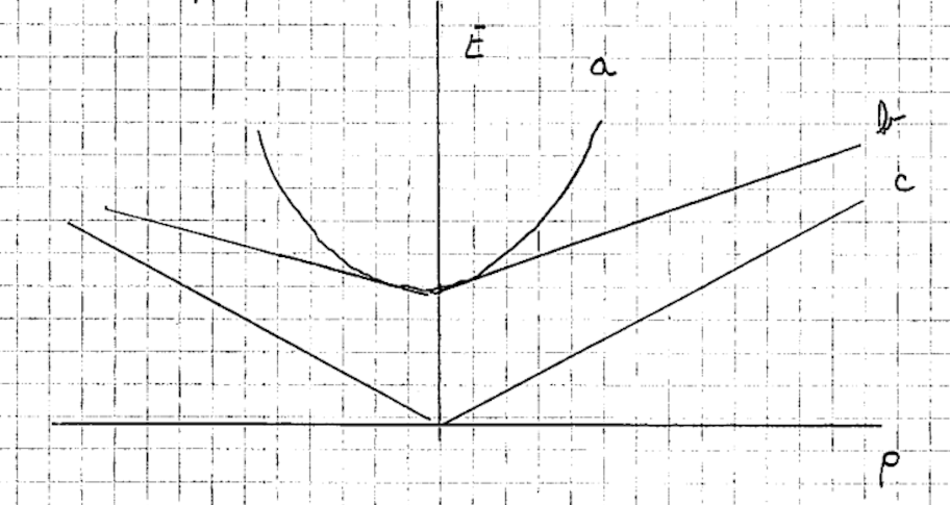
\includegraphics[height=0.25  \linewidth]{graf.pdf}
		     
		        \caption{\centering Grafico con le relative Energie}
        \end{figure}
\end{solution}


\newpage
\begin{solution}
	 Il lavoro che serve per accelerare un elettrone è uguale all'energia cinetica $W = T = 10^5 \ \mathrm{eV} = (\gamma -1) \ m_0 c^2$. Dunque $\gamma = \frac{1}{m_0} +1 = 1.196$ \  mentre \ $v = \sqrt{1 - \frac{1}{\gamma^2}} \ c = 0.548 \ c \simeq 1.644 \cdot 10^8 m/s$. 
 
 \begin{enumerate}[label=(\textit{\roman*})]
 \item $\Delta t = \frac{l_0}{v} = 6.08 \cdot 10^{-8} \ \mathrm{s}$ 
 
 \item $\Delta t' = \gamma \Delta t = 8.13 \cdot 10^{-8} \; \Rightarrow \; l'_0 = v \cdot \Delta t' = \gamma \cdot l_0 = 1.196 \cdot 10 \ \mathrm{m}$
 \end{enumerate}
\end{solution}



\begin{solution}
	  Considerando che l'energia incidente è $E_i$ e quella riflessa è $E_r$ si applica la conservazione del momento e dell'energia: 

  \begin{equation*}
       \begin{cases}
       \frac{E_i}{c} = \gamma m_0 v - \frac{E_r}{c}  \  \Rightarrow  \  E_i + E_r = \gamma m_0 \ v \ c \\
       E_i + m_0 c^2 = \gamma m_0 c^2 + E_r  \  \Rightarrow  \  E_i - E_r = m_0 c^2 (\gamma - 1) 
       \end{cases}
  \end{equation*}

  
  Quindi l'energia è:   $  \  2 E_i = m_0 c \ [\gamma \ v + c \ (\gamma -1)]  \  \Rightarrow  \  E_i = \frac{m_0}{2} \ c^2 \ [\gamma \ (\beta + 1) - 1] $. 
  
  \medskip
  La massa equivalente è dunque: \begin{equation*}
      M_e = \frac{E_i}{c^2} = \frac{m_0}{2} \ [\gamma \ ( \beta + 1) -1] 
  \end{equation*}
\end{solution}


\begin{solution}
\vspace{-1cm}
\begin{enumerate}[label=(\textit{\roman*})]
	  \item $
     T = (\gamma -1) m c^2  \Rightarrow  \gamma = 3  \ \  \text{quindi}  \ v = \sqrt{1 - \frac{1}{\gamma^2}} \ \  c = 0.94, \ \ c   p = m \gamma c = 2.82 \ m \ c $

 \item $T = (\gamma -1) m c^2  \Rightarrow  \gamma = 6  \ \ \text{quindi} \ \ v = \sqrt{1 - \frac{1}{\gamma^2}} \ c = 0.986 \  \ c  p = m \gamma c = 5.916 \ m \ c$
 \end{enumerate}
\end{solution}

\newpage
\begin{solution}
\vspace{-1cm}
\begin{enumerate}[label=(\textit{\roman*})]
	 \item $
     v_e =\frac{99}{100} \ c  \  \gamma = \frac{1}{\sqrt{1 - \left(\frac{99}{100}\right)^2}} = 7.1  \  \Rightarrow  \  T = (\gamma -1) \ m_e c^2 = 3.1 \cdot 10^6 \mathrm{eV}$
  
 Quindi $V = 3.1 \cdot 10^6 \mathrm{V}$.
 
\item $v_p =\frac{99}{100} \ c  \  \gamma = \frac{1}{\sqrt{1 - \left(\frac{99}{100}\right)^2}} = 7.1  \  \Rightarrow  \  T = (\gamma -1) \ m_p c^2 = 5.7 \cdot 10^9 \mathrm{eV} $

Quindi $V = 5.7 \cdot 10^9 \mathrm{V}$.
 \end{enumerate}


\end{solution}



\newpage
\markboth{SOLUZIONI}{3. Decadimenti e collisioni}
\subsection{Decadimenti e collisioni}
\begin{solution}
\vspace{-1cm}
\begin{enumerate}[label=(\textit{\roman*})]
\item Si ricorda che la condizione per cui esiste l'angolo massimo è che $\beta_{CM} > \beta^{\ast}_{\alpha}$, per cui si calcolano direttamente le velocità:
 
 	\begin{gather*}
     \beta_\mathrm{CM} = \beta_\pi = \frac{\overline{p}_\pi}{E_\pi} =  \frac{\overline{p}_\pi}{m_\pi \gamma} = \frac{\overline{p}_\pi}{m_\pi} \ \sqrt{1 - \beta^2_\pi} \hspace{1cm}
     \Rightarrow  \boxed{\beta_\pi = 0.96}
 	\end{gather*}
 	\begin{gather*}
     \beta^\ast_\mu = \frac{\overline{p^\ast}_\mu}{E^\ast_\mu} = \frac{\sqrt{E^{\ast 2}_\mu - m^2_\mu} \ 2 m_\pi}{m^2_\pi + m^2_\mu} = 0.27
 	\end{gather*}
     Dove  $E^\ast_\mu = \frac{m^2_\pi + m^2_\mu}{2 m_\pi} $. Dunque si ottiene che:
	
	\begin{equation*}
	    \begin{cases}
	    \not\exists \theta^\nu_\mathrm{MAX} \\
	    \theta^\mu_\mathrm{MAX} = \arcsin{\frac{p^\ast_\mu}{\gamma_\pi \beta_\pi m_\mu}} = 0.086 \ \mathrm{rad}
	    \end{cases}
	\end{equation*}
	 
	\item Se $E_\mu = \gamma (E^\ast_\mu + \beta_\pi \overline{p}_\mu \cos{\theta^\ast})$ si ottengono $E^\mu_\mathrm{MAX} = \gamma (E^\ast_\mu + \beta_\pi \overline{p}_\mu) = 495 \ \mathrm{MeV}$ e $E^\mu_\mathrm{MIN} = \gamma (E^\ast_\mu - \beta_\pi \overline{p}_\mu) = 290 \ \mathrm{MeV}$ . 
 
	Dunque $\Delta E_\mu = 205 \ \mathrm{MeV}$

	\item Considerando dal testo che $ 400 \le \overline{p}_\mu \le 450$ si ottiene: 
 	
 	\begin{gather*}
	     \rho = \frac{\int_{E_2}^{E_1} dE}{\Delta E} = 0.234 = 23.4 
	\end{gather*}
	Dove $E_2 = \sqrt{m_\mu + \overline{p}_\mu} = \sqrt{m_\mu + 450} = 414 \ \mathrm{MeV}$ e $
	     E_1 = 414 \ \mathrm{MeV}$
\end{enumerate}
\end{solution}

\newpage
\begin{solution}
\vspace{-1cm}
	\begin{enumerate}[label=(\textit{\roman*})]
		\item Considerando la soluzione della legge dei decadimenti in cui $N(t)$ è uguale al numero di particelle che ancora non sono decadute, si ottiene una relazione in cui il tempo è in funzione della velocità:
		\begin{align*}
	    & N(t) = N_0 \ e^{-\frac{t}{\tau}} = N_0 \ e^{-\frac{t}{\gamma \tau_0}} \\
	    & t = -\ln{\left( \frac{9}{10}\right)} \gamma \tau_0 \qquad \text{con} \; t = \frac{l}{\beta c} \\
	    & \frac{l}{\beta c } = \ln\left({\frac{10}{9}}\right) \frac{1}{\sqrt{1-\beta^2}} \tau_0  \\
	    & \frac{\beta}{\sqrt{1-\beta^2}} = \frac{l}{c \tau_{0} \ln \left(\frac{10}{9}\right) = 12.168} 
	   	\end{align*}
	quindi $\beta_{CM} = \beta_{\pi^-} = 0.997$ e di conseguenza $\gamma = 12.21$.
		 
	\noindent \textbf{N.B.} nella legge dei decadimenti quando viene riportato $\tau_0$ esso è misurato nel s.d.R. delle particelle, che quindi deve essere moltiplicato per il fattore $\gamma$ per spostarsi nel s.d.R. del laboratorio.
		
	Applicando la definizione di energia si ottiene $E = m_\pi c^2 \gamma = 1.709 \ \mathrm{GeV}$.
	
	\item La condizione per cui si ha un angolo $\theta > \frac{\pi}{2}$ si ottiene nel caso in cui $\beta_{CM} < \beta^\ast_\alpha$. Infatti basta riprendere il concetto secondo cui l'ellisse è il luogo dei punti su cui varia il modulo di $\overline{p}_\alpha$ e l'angolo di diffusione, e ricordarsi il caso in cui l'origine $(0;\ 0)$ è un punto interno all'ellisse. Si calcola dunque $\beta^\ast_\alpha = \beta^\ast_\mu$:
	
	\begin{align*}
		E^\ast_\mu &= \frac{m^2_\pi + m^2_\mu}{2 m_\pi} = 110 \ \mathrm{MeV} \\
	    \beta^\ast_\mu &= \frac{\overline{p^\ast}_\mu}{E^\ast_\mu} = \frac{\sqrt{(E^\ast_\mu)^2 - (m_\mu)^2}}{E^\ast_\mu} = 0.277
	\end{align*}	
	In conclusione avendo $\beta_\pi > \beta^\ast_\mu$ non si ha la condizione per cui l'angolo di diffusione $\theta > \frac{\pi}{2}$.
\end{enumerate}

\end{solution}
 
 
\newpage
\begin{solution}
\begin{enumerate}[label=(\textit{\roman*})]
\vspace{-1cm}
\item L'energia minima che deve avere il fotone, $\gamma$, per dare luogo alla reazione non è altro che l'energia di soglia. Si ha quindi la condizione per cui $p^\ast_p = 0 , \ p^\ast_n = 0 , \ p^\ast_\pi = 0$, ovvero la condizione per cui le particelle prodotte dal decadimento sono in quiete rispetto al centro di massa.
Sfruttando l'invariante di Mandelstam, $W^2$, in cui il primo membro fa riferimento al s.d.R. del lab e il secondo al s.d.R. del centro di massa, si ottiene:
\begin{align*}
(p_\gamma + p_T)^2 &= (p^\ast_p + 2 \ p^\ast_n + p^\ast_\pi)^2 \\ \Rightarrow [(p_\gamma + p_T)^0]^2 - (\overline{p}\gamma + \overline{p}T)^2  &= [(p^\ast_p + 2 \ p^\ast_n + p^\ast\pi)^0]^2 - (\overline{p^\ast}p + 2 \ \overline{p^\ast}n + \overline{p^\ast}\pi)^2
\end{align*}

\begin{align*}
(E\gamma + m_T)^2 - \overline{p}^2\gamma &= (m_p + 2 \ m_n + m_\pi)^2 \\
\Rightarrow E^S_\gamma &= \frac{(m_p + 2 \ m_n + m_\pi)^2 - m^2_T}{2 \ m_T} = 152.4 \ \mathrm{MeV}
\end{align*}
dove $p_\gamma = (E_\gamma, \overline{p_\gamma},0,0) = (E_\gamma, E_\gamma, 0, 0)$, 

$p_T = (E_T, 0, 0, 0) = (m_T, 0 , 0 , 0)$

$p^\ast_p = (m_p, 0, 0, 0)$

$p^\ast_n = (m_n, 0, 0, 0)$

$p^\ast_\pi = (m_\pi, 0, 0, 0)$.


N.B. $m_p = 938.3 \ \frac{\mathrm{MeV}}{c^2}$ e $m_n = 939.6 \ \frac{\mathrm{MeV}}{c^2}$
\end{enumerate}
\end{solution}


\begin{solution}
\vspace{-1cm}
\begin{enumerate}[label=(\textit{\roman*})]
\item La condizione per cui una particella viene emessa in avanti è data dal fatto che la distanza centro-origine è maggiore dell'asse maggiore dell'ellisse, ovvero:
\begin{equation*}
c.o. > s_x \ \ \Rightarrow \ \ \beta_{cm} > \beta^\ast_\alpha \ \ \Rightarrow \ \ \gamma_{cm} \beta_{cm} E^\ast_\alpha > \gamma_{cm} p^\ast_\alpha 
\end{equation*}
con $p^\ast_\alpha = \gamma_{cm} (p_{2,x} - \beta_{cm} m_\alpha) = -\gamma_{cm} \beta_{cm} m_\alpha$ si sostituisce e si ottiene la condizione:
\begin{gather}
\beta_{cm} \sqrt{m^2_{cm} + p^{\ast 2}\alpha} \ge p^\ast\alpha \ \Rightarrow \ \ m^2_{cm} + \beta^2_{cm} \gamma^2_{cm} m^2_\alpha \ge \gamma^2_{cm} m^2_\alpha \ \Rightarrow \ \ m^2_{cm} \ge m^2_\alpha \gamma^2 (1-\beta^2_{cm})  \\ \text{quindi} \ \ m_{cm} \ge m_\alpha 
\end{gather}
Dunque in questo caso ottengo che:
\begin{equation*}
\begin{cases}
\beta^\ast_\nu =1 \  \not\exists \text{ angolo di emissione perché} \ \not\exists \ \beta_{cm} > \beta^\ast_\nu \\
m_{cm} = m_e \  \exists \ \text{ angolo di emissione t.c. } \ \theta_{MAX} \le 90^0
\end{cases} 
\end{equation*}
\item Dalla massima energia delle particelle iniziali si vuole ottenere un'energia minima dei prodotti, per cui sfruttando l'invariante $t$ di Mandelstam si ottiene:
\begin{gather}
E^{'}{ \nu, min} = E\nu - \frac{2 \ p^\ast}{m_e} \ \ \Rightarrow \ \ \Delta E = E_\nu - E^{'}{ \nu, min} = \frac{2 \ p^\ast}{m_e} \\ \  \text{considerando che } \Rightarrow \ \ p^{\ast,2} = \frac{m^2_e E^2\nu}{m^2_e + 2 \ E_\nu m_e} 
\end{gather}
Quindi:
\begin{equation*}
f = \frac{\Delta E}{E_e} = \frac{2 \ p^\ast}{E_\nu \ m_e} = \frac{2 \ m_e E_\nu}{m^2_e+2 \ E_\nu m_e} = \frac{4}{5} = 80 \%
\end{equation*}
 
 \bigskip
 N.B. con il simbolo $'$ si indicano i prodotti;
 
 N.B. $E_\nu = p_\nu$ ; 
 \end{enumerate}
\end{solution}




\begin{solution}
	\begin{equation*}
    \pi^0_{(1)} \xrightarrow{} \gamma + \gamma 
 \end{equation*}
 \begin{equation*}
     \gamma + p \xrightarrow{} \pi^0_{(2)} + p 
 \end{equation*}
 \begin{equation*}
    \pi^0_{(2)} \xrightarrow{} \gamma + \gamma 
 \end{equation*}
 
 \begin{enumerate}[label=(\textit{\roman*})]
 	\item L'energia minima propria di $\pi^0_{(1)}$ per mettere in moto almeno un fotone con velocità $\beta_\gamma$ si ottiene come \ $E^{min}_\pi = m_\pi \ \gamma_\pi \ c^2$ . Dunque per stimare $\gamma_\pi$ si calcola l'energia di soglia del fotone nella reazione (2), sfruttando l'invariante di massa di Mandelstam : 
 \begin{equation*}
   (p_\gamma + p_p)^2 = (p_\pi + p_p)^2  \  \Rightarrow  \  E^S_\gamma = \frac{(m_\pi + m_p)^2 - m^2_p}{2 \ m_p} = 150 \ \mathrm{MeV} 
 \end{equation*}
 
 Si osserva che nella prima reazione nel s.d.R. del centro di massa $E^\ast_\gamma = \frac{m_\pi}{2}$, quindi applicando la trasformazione di Lorentz per l'energia: 
 
\begin{equation*}
    E^S_\gamma = \gamma_\gamma \ (E^\ast_\gamma + \beta_\gamma \ p^\ast_\gamma \ \cos{(\theta^\ast)}) = \gamma_\gamma \ E^\ast_\gamma \ (1 + \beta_\gamma)  \Rightarrow \boxed{ \beta_\gamma = \frac{\left(\frac{2 E^S_\gamma }{m_\pi} \right)^2 -1}{\left(\frac{2 E^S_\gamma}{m_\pi}\right)^2 + 1} = 0.64 = \beta_\pi}   
\end{equation*}
 
 In conclusione $E_\pi = m_\pi \ \gamma_\pi = m_\pi \frac{1}{\sqrt{1-\beta^2_\pi}} = 182.2 \ \mathrm{MeV}$
 
 \item L'angolo minimo tra i due $\gamma$ prodotti nella reazione (3) è uguale a 
 
 $\theta = 2 \ \arctg{\left( \frac{\beta^\ast_{\gamma}}{\gamma_{\pi_{(2)}} \beta_{\pi_{(2)}}} \right)}$ . 
 
 \smallskip
 Dato che la reazione (2) avviene in soglia si ha la condizione per cui i prodotti sono in quiete rispetto al centro di massa e dunque hanno la stessa velocità di quest'ultimo nel s.d.R. del laboratorio.
 
 Così, si impone che \ $\beta_{\pi_{(2)}} = \beta_{cm} = \frac{p_\gamma}{E^S_\gamma + m_p} = \frac{E^S_\gamma}{E^S_\gamma + m_p} = 0.14$ \ e \ $\gamma_{\pi_{(2)}} = 1 $ , mentre si ottiene $\beta^\ast_\gamma = 1$ perché $p^\ast_{\gamma} = E^\ast_\gamma$ . 
 
 In conclusione $\theta = 2.86 \ \mathrm{rad}$ .
 \end{enumerate}
 \end{solution}
 
 \bigskip



\begin{solution}
	 \begin{equation*}
     f^0 \xrightarrow{} \pi^0 + \pi^0
 \end{equation*}
 \begin{equation*}
     \pi^0 + \eta^0 \xrightarrow{} K^0 + K^0
 \end{equation*}
 
 \bigskip
 
 \begin{enumerate}[label=(\textit{\roman*})]
 	\item Nel laboratorio $E_f = E^S_\pi + 10 \ E^S_\pi = 10 E^S_\pi = m_f \ \gamma_f  \ \Rightarrow \ \beta_f = \sqrt{1-\left(\frac{1}{\gamma_f} \right)^2} = \sqrt{1 - \left(\frac{m_f}{10 E^S_\pi} \right)^2} $. 
 
 \bigskip
 Dato che la reazione (2) per uno dei due pioni $\pi^0$ è di soglia posso applicare la definizione di invariante di Mandelstam, per cui: 
 \begin{equation*}
     E^S_\pi = \frac{4 \ m^2_K - m^2_\eta - m^2_\pi}{2 \ m_\eta} = 0.7275 \ \mathrm{GeV} 
 \end{equation*}
  
  Quindi $\beta_f = 0.99$ 
  
  \item Sapendo che i due pioni hanno energia diversa i loro angoli non possono essere uguali, quindi si passa a calcolare la variazione di energia per trovare il valore del $\cos{\theta^\ast}$: 
 \begin{equation*}
     E^S_\pi = \gamma_f \  (E^\ast_\pi - \beta_f \ p^\ast_\pi)  \  [\text{minima}]    
 \end{equation*}
 \begin{equation*}
      9 \ E^S_\pi = \gamma_f \ (E^\ast_\pi + \beta_f \ p^\ast_\pi)  \  [\text{massima}] 
 \end{equation*}
 \begin{equation*}
     \Delta E_{LAB} = 9 \ E^S_\pi - E^S_\pi = \gamma_f \ (E^\ast_\pi + \beta_f \ p^\ast_\pi \ \cos{\theta^\ast} - E^\ast_\pi + \beta_f p^\ast_\pi \ \cos{\theta^\ast} ) = 2 \ \gamma_f \ \beta_f \ p^\ast_\pi \ \cos{\theta^\ast}         
 \end{equation*}
 
 \bigskip
 Quindi con \ $p^\ast_\pi = \sqrt{E^{\ast,2}-m^2_\pi} = 0.48 \ \mathrm{GeV}$ \  si ottiene \ $\cos{(\theta^\ast)} = \frac{4 \ E^S_\pi}{ \gamma_f \ \beta_f p^\ast_\pi} = 0.83$ \ e \ $ \sin{(\theta^\ast)} = \sqrt{1 - \cos^2{(\theta^\ast)}} = 0.57$ . 
 
 \bigskip
 Ricordando l'ellisse come il luogo dei punti in cui varia il momento, so che : 
 \begin{equation*}
     \tg{\theta_1} = \frac{p_y}{p_x} = \frac{p^\ast_\pi \ \sin{\theta^\ast_1}}{\gamma_f \ (p^\ast_\pi \cos{(\theta^\ast_1) + \beta_f \ E^\ast_\pi})} = \frac{\sin{\theta^\ast_1}}{\gamma_f \ \left(\cos{(\theta^\ast_1) + \frac{\beta_f}{\beta^\ast_\pi}}\right)} =  0.061 \ \mathrm{rad}     
 \end{equation*}
 
 \bigskip
 Dato che $\theta^\ast_2 = \pi - \theta^\ast_1 $ \ ottengo che \ $\sin{(\theta^\ast_2)} = \sin{(\theta^\ast_1)}$ \ e \  $\cos{(\theta^\ast_2)} = - \cos{(\theta^\ast_1)}$ , quindi: 
 
 \bigskip
 \begin{equation*}
     \tg{\theta_2} = \frac{p_y}{p_x} = \frac{p^\ast_\pi \ \sin{\theta^\ast_2}}{ \gamma_f \ (- \ p^\ast_\pi \cos{(\theta^\ast_2) + \beta_f \ E^\ast_\pi})} = \frac{\sin{\theta^\ast_2}}{\gamma_f \ \left(- \ \cos{(\theta^\ast_2) + \frac{\beta_f}{\beta^\ast_\pi}}\right)} =  0.274 \ \mathrm{rad}     
 \end{equation*}
 \end{enumerate}
 \end{solution}




\newpage
\subsection{Elettromagnetismo}
\begin{solution}
\vspace{-1cm}
\begin{enumerate}[label=(\textit{\roman*})]
\item Conoscendo i valori di $m$, $e$, $B$ ed $R^{\pm}$ si calcolano $p^{\pm} = \frac{e B R^{\pm}}{c}$ e considerando l'invariante di Mandelstan si stima la massa $M$:
\begin{gather*}
W^2 = p^2_X = M^2 = (p_{e^+} + p_{e^-})^2 \
= p^2_{e^+} + p^2_{e^-} + 2 \overline{p}{e^+} \cdot \overline{p}{e^+} \\
= 2 m^2 + 2 \mathcal{E}+ \mathcal{E}- - 2 p_{e^+} p_{e^+} \cos \alpha \\
= 2 m^2 + 2 \sqrt{m^2 + p^2_{e^+}} \sqrt{m^2 + p^2_{e^-}} - 2 p_{e^+} p_{e^+} \cos \alpha
\end{gather*}
Quindi $M = \sqrt{M^2}$.
\item In $S$ vale $t = \frac{L}{v} = \frac{L}{\beta c}$ mentre in $S'$ $\tau_0 = \frac{t}{\gamma} = \frac{L}{\gamma \beta c} = \frac{L}{\beta c} \sqrt{1-\beta^2}$. \
Applicando il principio di conservazione dell'energia:
\begin{gather*}
\mathcal{E}+ + \mathcal{E}- = \mathcal{E}X = M \gamma  \Rightarrow  \  \gamma = \frac{\mathcal{E}+ + \mathcal{E}-}{M} = \frac{\sqrt{m^2 + p^2{e^+}} + \sqrt{m^2 + p^2_{e^-}}}{M} \\ \Rightarrow  \beta^2 = 1 - \frac{M^2}{(\mathcal{E}+ + \mathcal{E}-)^2}
\end{gather*}
Dunque:
\begin{equation*}
\tau_0 = \frac{L M (\mathcal{E}+ + \mathcal{E}-)}{(\mathcal{E}+ + \mathcal{E}-) c \sqrt{(\frac{\mathcal{E}+ + \mathcal{E}-}{M})^2 - 1}} = \frac{L}{c \sqrt{(\frac{\mathcal{E}+ + \mathcal{E}-}{M})^2 - 1}}
\end{equation*}
\end{enumerate}
\end{solution}

\begin{solution}In S': $B' = 0$ mentre $E' = \frac{E}{\gamma}$. Inizialmente $\overline{p}_x(0) = 0$, $p^0(0) = \frac{\mathcal{E}}{c} = mc$.

\noindent Sempre in S':
\begin{equation*}
\begin{cases}
    p'_x(0) = \gamma \left(\overline{p}_x(0) - \frac{\beta}{c}p^0(0)\right) = -\gamma \beta m \\
    \\
\mathcal{E}'_0 = \sqrt{m^2 + \overline{p}'_x(0)^2} \\
\\
\frac{d\mathcal{E}'}{dt'} = \overline{F}' \cdot \overline{v}' = eE'\frac{dy}{dt}\end{cases} 
\end{equation*} 

Dato che conosco il valore di $\Delta \mathcal{E}$, trovo la relazione $\Delta y' = \Delta y = \frac{\Delta \mathcal{E}}{eE}$. La traiettoria seguita dalla particella è data da:

\begin{equation*} %le quazioni non insieme altrimenti esce fuori dalla pagina
y'(t) = \frac{\gamma}{eE} \left(\sqrt{\mathcal{E}'^2_0 + (ceE't')^2} - \mathcal{E}'_0 \right) = \frac{\Delta \mathcal{E}}{eE} \Rightarrow  t' = \sqrt{\left(\frac{\Delta \mathcal{E}}{\gamma} \right)^2 - 2 \frac{\Delta \mathcal{E}}{\gamma} \mathcal{E}'_0} \Rightarrow
\end{equation*}

\begin{equation*}
\boxed{ t = \gamma \left(t' - \frac{\beta}{c}x'(t) \right) }
\end{equation*} 
con
\begin{equation*}
x'(t) = \frac{p'_x(0) c}{eE'} \arcsinh \left(\frac{eE'ct'}{\mathcal{E}'_0} \right) 
\end{equation*}\end{solution}





\begin{solution}
Conoscendo i valori di $q$, $m$, $L$, $p_0$ e $R$ si indaga il moto della particella nel s.d.R. del LAB e nel s.d.R. S'. Scegliendo l'asse $x$ come l'asse in cui si ha il boost e, dunque, l'asse in cui avviene lo "spostamento" della particella si scegli di direzionare i campi come: $\overline{E} = (0,|E|,0)$ e $\overline{B} = (0,0,|B|)$.

Nel LAB la particella ha un moto alquanto complicato poiché essa è sottoposta alla forza di Coulomb dovuta alla presenza di $\overline{E}$, lungo l'asse $y$ (moto uniformemente accelerato), e ad un moto circolare dovuto alla presenza di $\overline{B}$. Sapendo che $\overline{E} \cdot \overline{B} = 0$ e che $B^2-E^2 > 0$ ci si può spostare nel s.d.R. S' in cui si ha solo il campo magnetico $B'= \frac{B}{\gamma}$ \ e i due campi sono legati dalla relazione $\beta = \frac{E}{B}$.

In S' si ha, dunque, solo un moto circolare uniforme nel piano $xy$. 
Si vogliono, ora, rivedere le grandezze di cui si hanno informazioni fino ad ora: 
$q, m, L, p_0, R$ \ e \ $\mathcal{E}_0 = \sqrt{m^2_q + p^2_{0,z}}$

Applicando il boost si ottengono:

\begin{equation*}
    p'_{0,z} = p_{0,z} = \beta \ \mathcal{E}_0;
\end{equation*}

\begin{equation*}
    p'_{0,x} = \gamma  \ (p_{0,x} - \beta \ \mathcal{E}_0) = \gamma  \beta \ \mathcal{E}_0;
\end{equation*}

\begin{equation*}
    \mathcal{E}'_0 = \gamma \ (\mathcal{E}_0 - \beta \ p_{0,x}) = \gamma \ \mathcal{E}_0.
\end{equation*}

Considerando il moto in S' si ricavano R e L: 
(nello specifico $L = \beta'_z \ T$ con $T$ periodo in cui la particella effettua una circonferenza e $\beta'_z = \frac{p'_{0,z}}{\mathcal{E}'_0} = \frac{p_{0,z}}{\mathcal{E}'_0}$)
\begin{equation*}
    T =  \frac{2\pi}{\omega_c} = \frac{2\pi m \gamma^2 c}{qB} =  \frac{2\pi  \gamma \ \mathcal{E}'_0}{qB} = \frac{2\pi  \gamma^2 \ \mathcal{E}_0}{qB};
\end{equation*}
\begin{equation*}
\begin{cases}
R = \frac{v'_\bot}{\omega_c} = \frac{v'_\bot \ m \gamma c}{q B'} = \frac{p'_{0,z} \ \gamma^2}{qB} = \frac{\gamma^2 \beta \ \mathcal{E}_0}{qB}  \  \Rightarrow  \  \gamma \beta = \frac{R \ 2\pi \gamma \ p_{0,z}}{\mathcal{E}_0 \ L}\\
\\
L = \beta'_z \ T = \frac{p_{0,z}}{\gamma \ \mathcal{E}_0} \ \frac{2\pi  \gamma^2 \ \mathcal{E}_0}{qB}  = \frac{2\pi \gamma \ p_{0,z}}{ qB}  \  \Rightarrow  \  B = \frac{2\pi \gamma \ p_{0,z}}{q L}
\end{cases}
\end{equation*}
Risolvendo rispetto a $\gamma$ si ottengono $\gamma = \sqrt{\left(\frac{R \ 2\pi \ p_{0,z}}{\mathcal{E}_0 \ L}\right)^2 + 1}$ \  e  \ $\beta = \sqrt{1 - \frac{1}{\gamma^2}} = \frac{\sqrt{\gamma^2-1}}{\gamma}$.
\begin{equation*}
    B = \frac{2\pi \ p_{0,z}}{q L} \ \sqrt{\left(\frac{R \ 2\pi \ p_{0,z}}{\mathcal{E}_0 \ L}\right)^2 + 1}  \  \Rightarrow  \  E = \beta B = \ \frac{2\pi \ p_{0,z}}{q L} \ \frac{R \ 2\pi \ p_{0,z}}{\mathcal{E}_0 \ L} = \frac{4\pi^2 R \ p^2_{0,z}}{q \ \mathcal{E}_0 \ L^2}
\end{equation*}

\end{solution}


\newpage
\subsection{Prove d'esame}
\begin{solution}
\begin{equation}\label{eq: dec5.1}
    \pi^+ \rightarrow \mu^+ + \nu
\end{equation}
\begin{enumerate}[label=(\textit{\roman*})]
	\item Per calcolare l'istante di tempo $\overline{t}$ si considera che il moto della particella si scompone in due. Si passa, però, prima al calcolo del momento e dell'energia nel s.d.R. S': \begin{equation*}
   p'_x = \gamma \ (0 - \beta \ \mathcal{E}_0) = - \gamma \ m_\pi = - 200 \ \mathrm{MeV/c}   
\end{equation*}
\vspace{-6mm}
\begin{equation*}
   \mathcal{E}'_0 = \gamma \ (\mathcal{E} - 0) = 250 \ \mathrm{MeV}   
\end{equation*}

Il moto è scomponibile in: 
\begin{equation*}
    \begin{cases}
    z(\overline{t'}) = \frac{d}{2} = 1 = \frac{\mathcal{E}'_0}{eE'} \ \sqrt{1+ \left(\frac{eE'}{\mathcal{E}'_0} \ c\overline{t'}\right)^2} -1 \\
    \\
    x(\overline{t'}) = \frac{p'_x}{E'} \ \arcsinh{\frac{eE'}{\mathcal{E}'_0} \ c\overline{t'}}  
    
    \end{cases}
\end{equation*}

\bigskip
Per ottenere l'istante nel s.d.R. del LAB bisogna applicare la trasformazione di Lorentz stimando il tempo \ $\overline{t'} = 5.4 \cdot 10^{-9}$ s dall'equazione con $z(\overline{t'})$ e il valore di $x(\overline{t'}) = -0.95 $ m.
Infatti: \begin{equation*}
    \overline{t} = \gamma \ \left(\overline{t'} - \frac{\beta}{c} \ x(\overline{t'}) \right) = 4.8 \cdot 10^{-9} \ \mathrm{s} 
\end{equation*}

 
\item  L'energia nel LAB si ottiene applicando la trasformazione di Lorentz, conoscendo l'energia $\mathcal{E}'_\pi$ e considerando che il momento $p'_x$ non dipende dal tempo:
\begin{equation*}
    \mathcal{E}'_\pi = \sqrt{\mathcal{E}'^2_0 + (eE'c\overline{t})^2} = 5.5 \cdot 10^{8} \ \mathrm{eV}  \  \Rightarrow  \  \mathcal{E}_\pi = \gamma \ (\mathcal{E}'_\pi + \beta \ p'_x) = 644 \ \mathrm{MeV} 
\end{equation*}

\item Nel s.d.R. del CM si ha: \begin{equation*}
    \mathcal{E}^\ast_\mu = \frac{m^2_\pi + m^2_\mu}{2 \ m_\pi} = 108.3 \ \mathrm{MeV} \ ;  \  p^\ast_\mu = \sqrt{\mathcal{E}^{\ast \ 2}_\mu + m^2_\mu} = 41.67 \ \mathrm{MeV}  \  \Rightarrow  \  \beta^\ast_\mu = 0.385  
\end{equation*}

\item Si, nel s.d.R. del condensatore la particella $\mu$ avrà un angolo di emissione massima perché la condizione $\beta = \frac{4}{5} \ > \ \beta^\ast_\mu = 0.385$ è verificata.
\end{enumerate}
\end{solution}

\newpage
\begin{solution}
\begin{equation}
    \label{eq: dec5.2}
    \gamma + p^+ \rightarrow p^+ + K^o
\end{equation}
\begin{enumerate}[label=(\textit{\roman*})]
\item \ La velocità $\beta_K$ nel s.d.R. del LAB è uguale a quella del CM poiché la reazione \ref{eq: dec5.2} avviene in soglia. Dunque, applicando l'invariante di Mandelstam $s$ si stima l'energia del fotone che verrà considerata per la velocità del CM: \begin{equation*}
 m^2_\gamma + m^2_p + 2 \ \mathcal{E}_\gamma m_p = (m_p + m_K)^2 \Rightarrow \boxed{ \mathcal{E}_\gamma = \frac{(m_p + m_k)^2 - m^2_p}{2 m_p} = 0.625 \ \mathrm{GeV} } \  \ p_\gamma = \mathcal{E}^2_\gamma 
\end{equation*}

Quindi: \begin{equation*}
\beta_{CM} = \beta_K = \frac{p_\gamma }{\mathcal{E}_\gamma + m_p} = 0.385  \  \Rightarrow  \  \gamma = 1.084   
\end{equation*}

\bigskip
\item \ Per stimare l'angolo minimo si calcola $\beta^\ast_\pi$: \begin{equation*}
 \mathcal{E}^\ast_\pi = \frac{m_K}{2} = 0.25 \ \mathrm{GeV/c}^2 \ ;  \  p^\ast_\pi = \sqrt{\mathcal{E}^{\ast \ 2}_\pi - m^2_\pi} \ ;  \  \Rightarrow  \  \beta^\ast_\pi = \frac{p^\ast_\pi}{\mathcal{E}^\ast_\pi} = 0.828  
\end{equation*}

\bigskip
\item \ Sapendo che $R^{\pm} = \frac{p_\bot c}{e B}$ si calcola $p_\bot$ partendo dall'energia e considerando che $\theta^\ast = \frac{\pi}{2}$: \begin{equation*}
   \mathcal{E}_\pi = \gamma \ \mathcal{E}^\ast_\pi = 0.271 \ \mathrm{GeV}  \  \Rightarrow  \  p_\pi = \sqrt{\mathcal{E}^{\ast \ 2}_\pi - m^2_\pi} = 0.232 \ \mathrm{GeV/c} 
\end{equation*}

Quindi: \begin{equation*}
R^{\pm} = 0.232 \ \mathrm{m}    
\end{equation*}
\end{enumerate}
\end{solution}





\begin{solution}
\begin{equation}\label{eq: dec5.3}
    p + D \rightarrow p + p + n 
\end{equation}
\begin{enumerate}[label=(\textit{\roman*})]
	\item Dato che $\overline{E} \cdot \overline{B} = 0$ e che $B^2 - E^2 > 0$ , esiste un s.d.R. S' in cui $E' = 0 $ ,  $B' = \frac{B}{\gamma}$ \ ,  \ $\beta = \frac{E}{B} = 0.1 \ \mathrm{V/m}$ \ e \ $\gamma = 1.005$ .

Si passa dunque al s.d.R. S' in cui sarà presente solo il campo $\overline{B'}$ e in cui i protoni compiono una traiettoria circolare di raggio $R$. In tale s.d.R. il momento é: \begin{equation*}
   p'_x = \gamma \ (p_x - \beta \mathcal{E}) = -\gamma \ \beta \mathcal{E} = - \gamma \ \beta m \gamma c^2 = - \gamma^2 \ \beta m = -0.101 \ \mathrm{GeV/c} \ ; \ \ p'_y = p'_z = 0  \ ;   
\end{equation*}

Partendo dall'origine i protoni effettuano una circonferenza in senso orario e arrivano all'ordinata $y_0 = 2R$ che vale: 
\begin{equation*}
    y_0 = 2R = \frac{v'_\bot}{\omega_c} = \frac{v'_\bot m \gamma c}{eB'} = \frac{v'_\bot m \gamma^2 c}{eB} = \frac{p'_\bot \ \gamma}{eB} = \frac{p'_x \ \gamma}{eB} = 1.02 \ \mathrm{m} 
\end{equation*}
\item Per ottenere il quadrimomento el s.d.R. del LAB si applicano le trasformazioni di Lorentz relative all'energia e al momento: 
\begin{equation*}
    \mathcal{E}_p = \gamma \ (\mathcal{E}'_p + \beta \ p'_x) = 1.0202 \ \mathrm{GeV} 
\end{equation*}
\vspace{-4mm}
\begin{equation*}
    p_x = \gamma \ (p'_x + \beta \  \mathcal{E}'_p) = 0.203 \ \mathrm{GeV/c} 
\end{equation*}

Quindi: $p_p = (E_p , p_x , 0 , 0)$ 
\item Tenendo conto dei valori delle masse come $m_N = m_p + 2 \ \mathrm{MeV/c}^2 = 1.002 \ \mathrm{GeV/c}^2$ \ e \ $m_D = 2 \ \mathrm{GeV/c}^2$  si procede alla verifica della reazione stimando se l'energia dei protoni calcolata nel punto precedente è maggiore o almeno uguale all'energia di soglia della reazione \ref{eq: dec5.3}. Quest'ultima si ottiene applicando l'invariante di Mandelstam: \begin{equation*}
    \mathcal{E}^S_p = \frac{(2m_p + m_N)^2 - m^2_p - m^2_D}{2 m_D} = 1.003 \ \mathrm{GeV}  \  \Rightarrow  \  \mathcal{E}_p = 1.0202 > \  \mathcal{E}^S_p = 1.003  
\end{equation*}

La reazione può dunque avvenire.
\end{enumerate}
\end{solution}




\begin{comment}
\begin{solution}
	In questo caso il testo del problema è sbagliato e non ci è stato dato un testo alternativo.
\end{solution}
\end{comment}


\begin{solution}
\begin{equation} \label{eq: dec5.1.1}
     K \rightarrow \pi^- + \pi
 \end{equation}
 

 \begin{equation}
  \label{eq: dec5.1.2}
     \pi^- \rightarrow \mu^- + \nu^-_\mu
 \end{equation}
 
 \begin{enumerate}[label=(\textit{\roman*})]
 	\item Per capire cosa accade al fascio di pioni $\pi^-$ bisogna conoscerne l'energia $\mathcal{E}_\pi$ e il momento $p_\pi$ nel s.d.R. del LAB per poi spostarsi in quello del condensatore. Sapendo che tra i due pioni si ha un angolo minimo $\theta_m = \frac{\pi}{2}$ si può calcolare la velocità relativa $\beta^{CL}$ tra i s.d.R. del CM e del LAB, stimando prima $\beta^\ast$ nel CM: 
\begin{equation*}
    \mathcal{E}^\ast = \frac{m_K}{2} = 0.25 \ \mathrm{GeV/c}^2 \ \Rightarrow \ p^\ast_\pi = \sqrt{\mathcal{E^\ast}^2_\pi - m^2_\pi} = 0.207 \ \mathrm{GeV/c} \ \Rightarrow \ \beta^\ast_\pi = \frac{p^\ast_\pi}{\mathcal{E}^\ast_\pi} = 0.828  
\end{equation*}

Quindi \begin{equation*}
     \theta_m = 2 \arctg{\left(\frac{\beta^\ast}{\gamma^{CL} \ \beta^{CL}} \right)}  \  \Rightarrow  \  \beta^{CL} = 0.638  \  \Rightarrow  \  \gamma^{CL} = 1.298 
 \end{equation*}
 A questo punto si calcolano l'energia e il momento nel s.d.R. del LAB: \begin{equation*}
     \mathcal{E}_\pi = \gamma^{CL} \ (\mathcal{E}^\ast_\pi + \beta^{CL} \ p^\ast_\pi \cos{(\theta^\ast)}) =0.325 \ \mathrm{GeV}   \  \Rightarrow  \  p_\pi = \sqrt{\mathcal{E}^2_\pi - m^2_\pi} = 0.293 \ \mathrm{GeV/c}  
 \end{equation*} 
 con $\theta^\ast = \frac{\pi}{2}$ visto che si ha $\theta_m$ . Per capire che tipo di moto ha nel s.d.R. del condensatore è il caso di applicare nuovamente le trasformazioni di Lorentz considerando però $\beta = \frac{3}{5}$, $\gamma = \frac{5}{4}$ e che il boost è sempre lungo $x$. Si stimano i momenti $p'_x$, $p'_y$ e $p'_\bot$ considerando che il momento $p_\pi$ è solo lungo y (come sottolinea il testo del problema): 
 \begin{equation*}
     p'_x = \gamma \ (0- \beta \\\mathcal{E}_\pi ) = 0.243 \ \mathrm{GeV/c}   \  \Rightarrow  \  p'_y = p_\pi  \  \Rightarrow  \  p'_\bot = \sqrt{p'^2_x + p'^2_y} = 0.381 \ \mathrm{GeV/c} 
 \end{equation*}
 Con $\alpha = \arctg{\left( \frac{p'_x}{p'_y}\right) = 0.69}$ rad. 
 
 Tramite i seguenti disegni è possibile capire meglio tale moto e notare che il percorso che viene effettuato all'interno del condensatore è un arco di circonferenza: 
 
 \begin{figure}[h]
\begin{flushright}

	    \begin{minipage}[]{.49\textwidth}
	       \begin{figure}[H]
	        	\flushright
    		    \hspace{-1cm}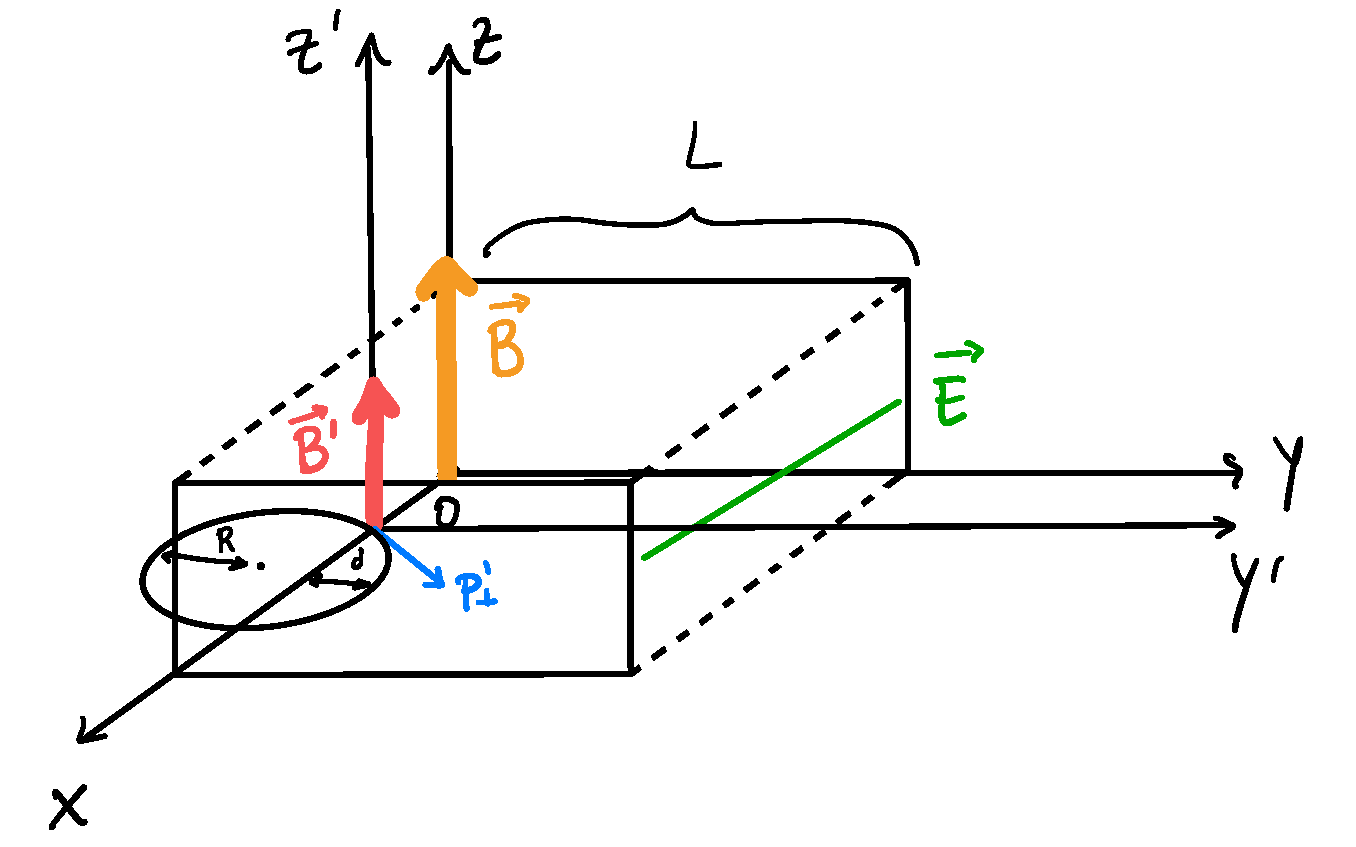
\includegraphics[height=0.60   \linewidth]{condensatore.pdf}
		        
        \end{figure}

		\end{minipage}
	        \hspace{1mm}%
		\begin{minipage}[]{.49\textwidth}
			\begin{figure}[H]
	        	\flushright
    		    \hspace{-1cm}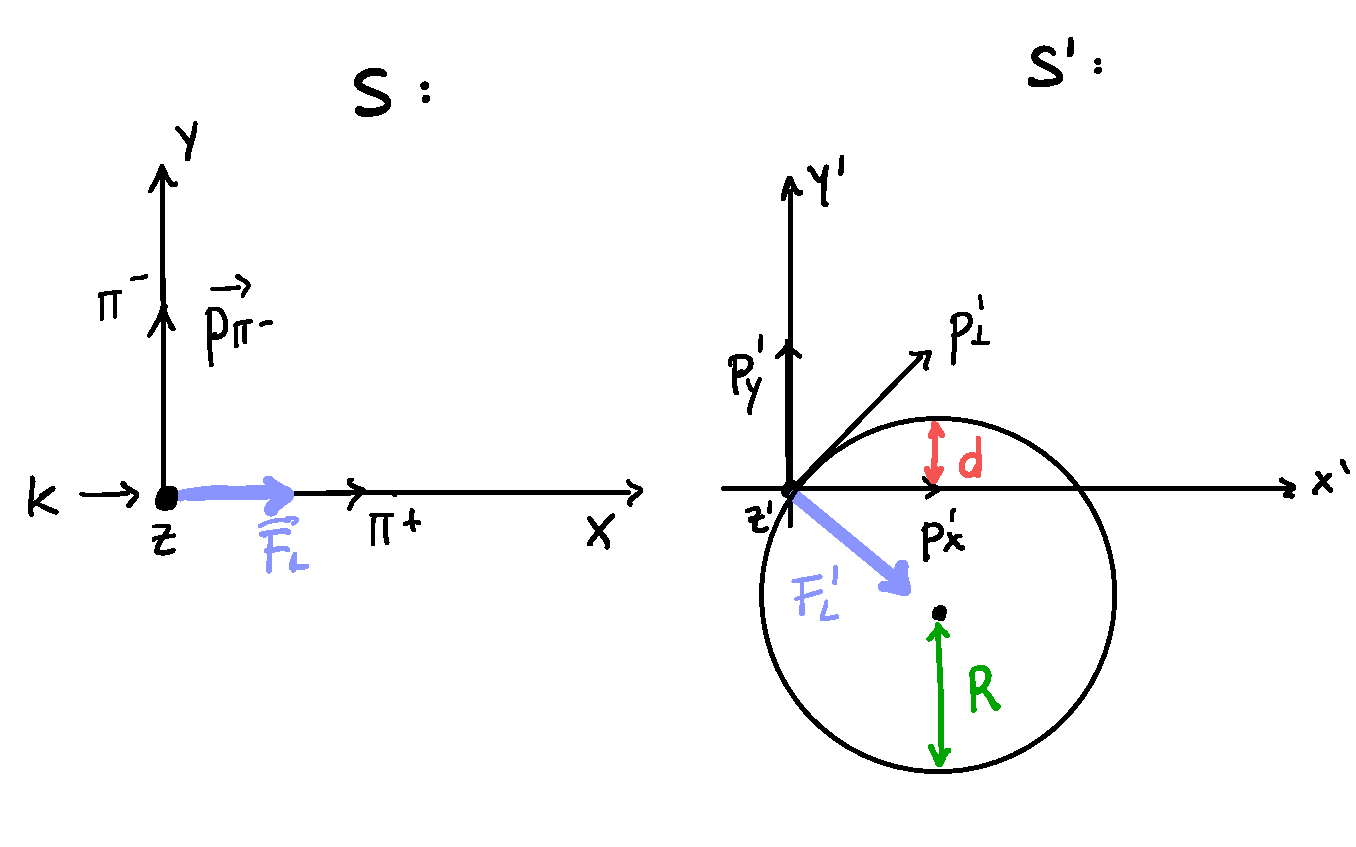
\includegraphics[height=0.70   \linewidth]{ss.pdf} 
    		    
        \end{figure}
		  \end{minipage}
    \end{flushright}
	\end{figure}
 

Tutti questi passaggi servono per capire se il fascio di pioni $\pi^-$ escono dallo stesso lato del condensatore o se lo attraversano. In quest'ultimo caso bisognerebbe considerare che l'energia del fascio non è la stessa ma varia rispetto considerando anche la componente del campo elettrico $E$: $\Delta \mathcal{E} = eE \ \Delta y$. 

Si passa, dunque, a calcolare la distanza $d$ per cui il fascio entra e si verifica se $d < L$ o $d > L$: 
\begin{equation*}
    R = \frac{p'_\bot}{ceB'} = 1.9 \ \mathrm{m}  \  \Rightarrow  \  R\ (1-\sin{(\alpha)}) = 0.69 \ \mathrm{m}  \  \Rightarrow  \  d = 0.69 < L = 1  
\end{equation*}

L'energia è dunque soltanto quella della particella $\mathcal{E}_\pi = 0.325 \ \mathrm{GeV/c}$ .

\item Per dimostrare e stimare gli angoli massimi delle singole particelle nel s.d.R. del LAB rispetto alla linea di volo di $\pi^-$ si verifica la condizione di esistenza per cui $\beta^\ast_\alpha < \beta_{CM}$. Il decadimento \ref{eq: dec5.1.2} fa si che $\beta_{CM} = \frac{p_\pi}{\mathcal{E}_\pi} = 0.90$ \ e \ $\gamma_{CM} = 2.3$ \ . Quindi: \begin{equation*}
    \not\exists \theta^{max}_\nu \  \text{ perché } \beta^\ast_\nu > \beta_{CM}  \  
\end{equation*}
mentre sapendo che $\mathcal{E}^\ast_\mu = \frac{m^2_\pi + m^2_\mu}{2 \ m^\pi} = 0.109$ GeV e che $p^\ast_\mu = 0.031 $ GeV/c si ha che:   \begin{equation*}
    \beta^\ast_\mu = \frac{p^\ast_\mu}{\mathcal{E}^\ast_\mu} = 0.281  \  \Rightarrow  \  \theta^{max}_\mu = \arcsin{\left(\frac{p^\ast_\mu}{\gamma_{CM} \ \beta_{CM} \ m_\mu}\right)} = 0.14 \ \mathrm{rad} = 8.2^\mathrm{o} 
\end{equation*}

\item $\mathcal{E}^{max}_\mu = \gamma_{CM} \ (\mathcal{E}^\ast_\mu + \beta_{CM} \ p^\ast_\mu \ \cos{(\theta^{max}_\mu)}) = 0.314 \ \mathrm{GeV}$

\item Applicando l'invariante di Mandelstam: \begin{equation*}
    (p_\pi - p_\nu)^2=(p_\mu - 0)^2  \  \Rightarrow  \  \mathcal{E}_\nu = \frac{m^2_\pi - m^2_\mu}{2 \ \mathcal{E}_\mu} = 0.0132 \ \mathrm{GeV} 
\end{equation*}

Per la conservazione del momento si può considerare che $p_\pi = p_\mu \ \cos{(\theta_\mu)}$ \ e che \ $ p_\nu = p_\mu \ \sin{(\theta_\mu)}$ per stimare l'angolo $\theta_\mu$: 
\begin{equation*}
    \tan{(\theta_\mu)} = \frac{p_\nu}{p_\pi}  \  \Rightarrow  \  \theta_\mu = \arctg{\left( \frac{p_\nu}{p_\pi}\right)} = 2.58^{\mathrm{o}} 
\end{equation*}
\end{enumerate}
\end{solution}





\begin{solution}
\begin{equation}\label{eq: dec5.6}
    \pi^+ \rightarrow \mu^+ + \nu 
\end{equation}

\begin{enumerate}[label=(\textit{\roman*})]
	\item La velocità minima che devono avere i muoni per colpire il bersaglio si ottiene considerando che l'angolo $\theta$ si l'angolo di emissione in avanti e che valgano le seguenti relazioni: \begin{equation*}
 \theta = \arctg{\frac{L}{2} \ \frac{1}{L}} = 0.464 \ \mathrm{rad}  \  \Rightarrow  \  \beta_{\mathrm{min}} = \frac{p^\ast_\mu}{\sin{\theta} m_\mu} \ \frac{1}{\sqrt{1 + \frac{p^{\ast \ 2}}{\sin^2{\theta} m^2_\mu}}} = 0.533  \  \gamma = 1.182   
\end{equation*} 

considerando che \begin{equation*}
\mathcal{E}^\ast_\mu = \frac{m^2_\pi + m^2_\mu}{2 m_\pi} = 110.13 \ \mathrm{MeV}     \  \Rightarrow  \  p^\ast_\mu = \sqrt{\mathcal{E}^{\ast \ 2 }_\mu - m^2_\mu} =  29.87 \ \mathrm{Mev/c}  
\end{equation*}

\bigskip
Se si volesse considerare la distanza che effettua il muone, con $\beta_\mu = \frac{p_\mu}{\mathcal{E}_\mu}$ \ e \ $\gamma = \frac{\mathcal{E}_\mu}{m_\mu}$ , si avrebbe: \begin{equation*}
d = \beta c \ \gamma \ \tau^0_\mu  = \frac{p_\mu \ \tau^0_\mu \ c}{m_\mu}  = \frac{ \tau^0_\mu \ c}{m_\mu} \ \sqrt{\mathcal{E}^{2}_\mu - m^2_\mu} = \frac{ \tau^0_\mu \ c}{m_\mu} \ \sqrt{[\gamma \ (\mathcal{E}^\ast_\mu + \beta \ p^\ast_\mu \ \cos{\theta^\ast})]^{2} - m^2_\mu}  
\end{equation*}

Con \ $\cos{\theta^\ast_{\mathrm{max}}}= -\frac{\beta^\ast_\mu}{\beta}$ \ si ottiene: 
\begin{equation}
\label{eq: ese5.6}
 d = \frac{ \tau^0_\mu \ c}{m_\mu} \ \sqrt{[\gamma \ (\mathcal{E}^\ast_\mu - \beta^\ast_\mu \ p^\ast_\mu )]^{2} - m^2_\mu}   
\end{equation}

Si ha, dunque, una distanza che dipende dall'angolo e che decresce al decrescere dell'angolo stesso. 
Stimando la distanza considerando l'equazione \ref{eq: ese5.6} si ottiene $E_\mu = 120 \ \mathrm{MeV}$ \ e dunque \ $d = 358 \ \mathrm{m} \ > \sqrt{100^2 + 200^2} = 223.6 \ \mathrm{m} $

\item La velocità massima che bisogna stimare si ottiene considerando il caso più favorevole con \ $\theta = \theta^\ast = 0$. 
Si impone dunque che $L > d $ : \begin{equation*}
d =  \frac{ \tau^0_\mu \ c}{m_\mu} \  p(\theta= 0)_\mu =\frac{ \tau^0_\mu \ c}{m_\mu} \ \gamma \ (p^\ast_\mu + \beta \ \mathcal{E}^\ast_\mu) = \frac{ \tau^0_\mu \ c}{m_\mu} \ \gamma \ p^\ast_\mu  \ \left(1 + \frac{\beta}{\beta^\ast_\mu}\right) = L   
\end{equation*}

Risolvendo per $\beta$ si ottiene : \begin{equation*}
 \gamma \ \left(1 + \frac{\beta}{\beta^\ast_\mu}\right) = \frac{L m_\mu}{\tau^0_\mu \ c \ p^\ast_\mu } = a = 1.075  \  \Rightarrow  \  \left(1 + \frac{1}{\beta^\ast_\mu} \beta + 2 \frac{\beta}{\beta^\ast_\mu} + 1 - a^2  \right)  \  \Rightarrow  \  \beta = 0.02  
\end{equation*}

\item \ Per ogni $\beta $ la distanza massima che si può considerare è quella per cui $\theta = \theta^\ast = 0$ e per cui si ha: \begin{equation*}
 d =  \frac{ \tau^0_\mu \ c}{m_\mu} \ \gamma \ (p^\ast_\mu + \beta \ \mathcal{E}^\ast_\mu)  
\end{equation*}

che cresce al crescere di $\beta$ . La distanza $L_{\mathrm{max}}$ che non sarebbe altro che la $d_\mathrm{min}$ è dunque ottenibile nel caso in cui $\beta = 0$ \ e \ di conseguenza $\gamma = 1$, ovvero nel caso in cui le particelle decadono da ferme: \begin{equation*}
 d_{\mathrm{min}} = \frac{ \tau^0_\mu \ c}{m_\mu} \ p^\ast_\mu = 186 \ \mathrm{m}  \  \rightarrow  \   L > d_{\mathrm{min}} 
\end{equation*} 
\end{enumerate}
\end{solution}


\newpage
\subsection{Francesco Addari}
\begin{solution}
	Bisogna prestare attenzione al fatto che il tempo di vita medio è misurato nel sistema di riferimento solidale al moto dei $\pi^-$. Scriviamo la legge del decadimento nel sistema $\mathcal{S}'$ solidale ai pioni.
$$ N(t') = N_0 e^{- \frac{t'}{\tau_\pi}} $$
Il tempo di percorrenza dei pioni nel laboratorio, detta $\beta_\pi$ la velocità  in unità  di $c$ è
$$ \overline{t} = \frac{l}{c \beta_\pi} $$
Utilizzando la formula del tempo proprio, si ricava subito il tempo nel sistema $\mathcal{S}'$
$$ \overline{t}' = \frac{l}{c \beta_\pi \gamma_\pi} $$
Ora notando che $\frac{N(\overline{t}')}{N_0} = 0.9$ possiamo scrivere
$$ 0.9 = e^{-\frac{l}{c \beta_\pi \gamma_\pi \tau_\pi}}  \  \Rightarrow  \  
- \frac{\tau_\pi c}{l} \log 0.9 = \frac{\sqrt{1 - \beta_\pi^2}}{\beta_\pi}   \  \Rightarrow  \  
\beta_\pi = \sqrt{\frac{1}{1 + \frac{c^2 \tau_\pi^2 \log^2 0.9}{l^2}}} $$
Inserendo i valori si trova che $\beta_\pi = 0.997$ in unità  di $c$, da cui ricaviamo subito l'energia dei $\pi^-$, con la formula $\boldsymbol{\E_\pi = m_\pi \gamma_\pi = 1.7}$ \gras{GeV}.
\\
Controlliamo se esiste o meno un angolo massimo di emissione dei $\mu^-$ rispetto alla linea di volo dei $\pi^-$. Dobbiamo verificare che $\beta_\pi = \beta_{CM} > \beta_\mu^\star$ affinché possa esistere un $\theta_{MAX}$.
$$ \beta_\mu^\star = \frac{p^\star}{\E^\star}$$
Ora, utilizzando il fatto che $m_\nu \sim 0$ semplifichiamo l'espressione di $p^\star$ 
$$ p^\star = \frac{1}{2 m_\pi} \sqrt{m_\pi^4 + m_\mu^4 -2 m_\mu^2 m_\pi^2} = \frac{m_\pi^2 - m_\mu^2}{2 m_\pi} = \boldsymbol{30.6 \mbox{ \gras{MeV/c}}}$$
$$ \E^\star = \sqrt{p_\star^2 + m_\mu^2} = \boldsymbol{109.4 \mbox{ \gras{MeV}}}$$
Infine $\boldsymbol{\beta_\mu^\star = 0.28}$, dunque esiste l'angolo massimo di emissione, che sappiamo essere minore di $\frac{\pi}{2}$. Dunque i muoni non possono essere emessi all'indietro. 
\\
Per i neutrini la risposta è immediata, poiché avendo massa nulla viaggiano a velocità  $\beta_\nu = 1$ in ogni sdr. Dunque non hanno angolo massimo di emissione e possono essere emessi all'indietro.
\end{solution}
\newpage
\begin{solution}
	Innanzitutto è necessario fare delle scelte: definiamo il nostro sistema di riferimento $\mathcal{S}$ tale che 
$$ \vec{E} = (0, \modulo{E}, 0)  \  \vec{B} = (0, 0, \modulo{B})$$
Come si muove la particella in $\mathcal{S}$? Subirà  un'accelerazione diretta parallelamente all'asse $y$ per via del campo elettrico e il campo magnetico le fa compiere un'orbita. In più si muove di moto rettilineo lungo l'asse $z$ per via del momento iniziale. Dalle informazioni date ($B^2 - E^2 >0$) deduciamo che esiste $\mathcal{S}'$ ove il campo elettrico è nullo, e qui percorre dunque un'elica circolare. In definitiva capiamo che in $\mathcal{S}$ percorre un'elica non cilindrica tale che la sua proiezione è $2R$ lungo l'asse $y$ e ha passo $L$. La scelta di $\mathcal{S}$ fa si che per passare a $\mathcal{S}'$ è necessario fare un boost lungo l'asse $x$ con velocità  $\beta = \frac{E}{B}$ e ne consegue che $2R$ e $L$ rimangono invariati. Dunque in $\mathcal{S}'$ sappiamo che percorre un'elica cilindrica di cui sappiamo passo $L$ e raggio $R$. 
\\
Con una trasformazione di Lorentz troviamo il campo magnetico in $\mathcal{S}'$, che sarà  sempre in direzione dell'asse $z' \parallel z$
$$ B' = \gamma \tonde{B - \beta E} = \sqrt{B^2- E^2} = \frac{B}{\gamma}$$
Il momento iniziale, in direzione $z$, rimane invariato, mentre in $\mathcal{S}'$ ci sarà  un momento iniziale anche in direzione $x'$, che troviamo con una trasformazione di Lorentz
$$ p'_{0z'} = p_{0z}  \  p'_{0x'} = \gamma ( - \beta \E_0) $$
dove $\E_0  = \sqrt{m^2 + p_{0z}^2}$. Questo implica che l'energia iniziale in $\mathcal{S}'$ è
$$ \E'_0 = \gamma \E_0$$
\\
In $\mathcal{S}'$ l'energia e il modulo del momento rimangono costanti, quest'ultimo sia in direzione parallela al campo magnetico che in direzione perpendicolare. Dunque il modulo del momento in direzione perpendicolare è sempre $p'_{0x'}$. Possiamo scrivere il raggio dell'orbita in funzione dei dati noti
$$ R = \frac{p'_{0x'}}{q B'} = \frac{\gamma^2 \beta \E_0}{q B} $$
Ora conviene trovare il periodo dell'orbita così da trovare il tempo in cui percorre una lunghezza $L$ in direzione $z'$. 
$$ T = \frac{2 \pi}{\omega} = \frac{2 \pi \E'_0}{q  B'} = \frac{2 \pi \gamma^2 \E_0}{q  B} $$
Allora in direzione $z'$ percorre un moto rettilineo uniforme con punto iniziale $z'=0$ e velocità  $\beta_{z'} = \frac{ p_{0z}}{\E'_0}$ Allora
$$ L =  \beta_{z'} T =  \frac{p_{0z}}{\E'_0} \frac{2 \pi \E'_0}{q  B'}
= \frac{2 \pi \gamma p_{0z}}{q B} $$
Abbiamo dunque due equazioni e due incognite, dunque possiamo risolvere il sistema
$$ \begin{cases}
R =  \frac{\gamma^2 \beta \E_0}{q B} \\ \\
L = \frac{2 \pi \gamma p_{0z}}{q B}
\end{cases}  \  \Rightarrow  \  R = \frac{\E_0 L}{2\pi p_{0z}} \gamma \beta$$
Utilizzando ora il fatto che
$$ \beta = \frac{ \sqrt{\gamma^2 -1}}{\gamma}$$
$$ R = \frac{\E_0 L}{2\pi p_{0z}} \sqrt{\gamma^2 -1}  \  \Rightarrow  \ 
\gamma = \sqrt{\tonde{\frac{2 \pi R p_{0z}}{\E_0 L}}^2 + 1}$$
Scrivendo $\beta$
$$ \beta = \frac{\frac{2\pi R p_{0z}}{\E_0 L}}{\sqrt{\tonde{\frac{2 \pi R p_{0z}}{\E_0 L}}^2 + 1}}  \  \Rightarrow  \  
\beta \gamma = \frac{2\pi R p_{0z}}{\E_0 L} $$
$$ B =  \frac{\gamma \gamma \beta \E_0}{q R } = 
\frac{2 \pi p_{0z}}{qL} \sqrt{\tonde{\frac{2 \pi R p_{0z}}{\E_0 L}}^2 + 1} $$
Ora dal fatto che $E = \beta B$
$$ E = \frac{\frac{2\pi R p_{0z}}{\E_0 L}}{\sqrt{\tonde{\frac{2 \pi R p_{0z}}{\E_0 L}}^2 + 1}} \frac{2 \pi p_{0z}}{qL} \sqrt{\tonde{\frac{2 \pi R p_{0z}}{\E_0 L}}^2 + 1} = \frac{4 \pi^2 R p_{0z}^2}{q \E_0 L^2}$$
\end{solution}

\begin{solution}
Se diciamo la direzione $x$ quella in cui avviene l'urto, tale rimarrà  anche con un boost nella stessa direzione per passare dal sistema $\mathcal{S}$ al sistema del centro di massa.
\\
Il centro di massa nel proprio sistema di riferimento rimane chiaramente fermo. Ciò vuol dire che il momento totale del sistema, nel centro di massa, deve essere nullo. Questo ci dice che i muoni hanno momento nel centro di massa uguale e di verso opposto. Da questo ne consegue anche che hanno la stessa energia, in questo sdr. Il quadrimomento totale, prima dell'urto, è dunque
$$ P_{TOT}^{\alpha \star} = (2 \E^\star_+, 0,0,0) $$
La condizione limite perché la reazione avvenga, è che i $\tau$ siano prodotti in soglia, ossia siano prodotti fermi nel centro di massa. Allora in questo caso il quadrimomento totale, dopo l'urto, è
$$ P_{TOT}^{\alpha \star} = (2 M, 0,0,0) $$
Per la conservazione del quadrimomento ricaviamo subito che $M = \E^\star$. Da qui possiamo ricavare il momento nel centro di massa dei muoni
$$ p^\star_\pm = \pm \sqrt{M^2 - m^2}$$
Utilizzando le trasformazioni di Lorentz, e ricordando la scelta di porre l'asse parallelo al momento dei muoni, possiamo scrivere
$$ \E_+ = \gamma (\E^*_+ + \beta p_+^\star)  \  
p_+ = \gamma (p_+^\star + \beta \E^*_+) $$
$$ \E_- = \gamma (\E^*_+ - \beta p_+^\star)  \  
p_- = \gamma ( \beta \E^*_+ - p_+^\star ) $$
Ora, un dato noto è la velocità  $v_+$, e definiamo la corrispondente in unità  di $c$ $\beta_+$. Per questo motivo conosciamo anche $p_+$ e di conseguenza $\E_+$. Possiamo inoltre scrivere
$$ \beta_+ = \frac{p_+}{\E_+} = \frac{p_+^\star + \beta \E^*_+}{\E^*_+ + \beta p_+^\star}  \  \Longrightarrow  \  
\beta = \frac{-p_+^\star + \beta_+ \E_+^\star}{\E_+^\star - \beta_+ p_+^\star} = \frac{\beta_+ M - \sqrt{M^2 -m^2}}{M - \beta_+ \sqrt{M^2 -m^2}}$$
Una volta che conosco $\beta$ in funzione di dati noti, possiamo ricavare il valore $p_-$ con una delle trasformazioni di Lorentz scritte di sopra.
\\
Possiamo considerare l'evento come un decadimento, se troviamo la massa equivalente della situazione prima dell'urto, che non è la semplice somma delle masse. Infatti, dato un decadimento $M \rightarrow m_1 + m_2$ è vero che
$$ P^\mu P_\mu = M^2$$
Scriviamo questa quantità  scalare prima dell'urto, così da ricavare la massa equivalente $M_e$
$$ M^2_e =(P^\alpha_+ + P^\alpha_-)^2 = (P^\alpha_+)^2 + (P^\alpha_-)^2 + 2 P^\alpha_+ P^-_\alpha = 2m^2 + 2\E_+ \E_- -2 p_+ p_- \cos \theta $$ 
Ma siccome lo scontro è frontale, $\theta = \pi$. Dunque
$$ M_e = \sqrt{2m^2 + 2\E_+ \E_- + 2 p_+ p_-}$$
I dati sono tutti noti poiché conosco sia $p_+$ che $p_-$,che in generale assumiamo sia maggiore uguale a quello trovato precedentemente. A questo punto per trovare la velocità  dei tauoni nel centro di massa 
$$\beta_\tau^\star = \frac{2 p^\star_\tau}{M_e} = \sqrt{1 - 4\frac{m_\tau^2}{M_e^2}} $$
\end{solution}

\newpage
\begin{solution}
Innanzitutto è necessario fare delle scelte: definiamo il nostro sistema di riferimento $\mathcal{S}$ tale che la particella sia a $t=0$ nell'origine e 
$$ \vec{E} = (0, \modulo{E}, 0)  \  \vec{B} = (0, 0, \modulo{B})$$
Per comodità  di scrittura $\modulo{E} = E$ e $\modulo{B} = B$ d'ora in poi. La proiezione $L$ è dunque sull'asse $y$ e non cambia la sua lunghezza se faccio un boost in direzione $x$. Siccome $B^2 - E^2 < 0$ allora esiste un sistema di riferimento $\mathcal{S}'$ tale che $B' = 0$. La velocità  di $\mathcal{S}'$ rispetto a $\mathcal{S}$ è $\beta = \frac{B}{E}$. Calcoliamo il modulo del campo $E'$, che sarà  in direzione $y' \parallel y$.
$$ E' = \gamma \tonde{E - \beta B} = \sqrt{E^2 - B^2} = \frac{E}{\gamma} $$
Prima di lavorare però nel sistema in cui è presente solo campo elettrico, possiamo scrivere la legge di potenza in $S$, che non dipende dal campo magnetico
$$ \dtot{\E}{t} = e \SP \ps{\vec{v}}{\vec{E}} = e E v_y = e E \dtot{y}{t} 
 \  \Rightarrow  \  \Delta \E = e E \Delta y$$
Ma sappiamo che $\Delta y = L$, e che $\E = \Delta \E + \E_0$. Allora troviamo che $\boldsymbol{\E = m + eEL}$.
\\
A questo punto possiamo trovare il modulo del momento nell'istante in cui entra nella zona in cui è presente soltanto il campo magnetico
$$ \modulo{p} = \sqrt{\E^2 -m^2} = \sqrt{2 m eEL + \tonde{eEL}^2} = 
eEL \sqrt{\frac{2 m}{eEL} +1}$$
Il raggio è dunque
$$ R = \frac{\modulo{p}}{e B} = \frac{EL}{B}\sqrt{\frac{2 m}{eEL} +1} $$
Per ricavare l'istante in cui passa dalla prima alla seconda regione è necessario effettuare un boost con velocità  $\beta$ per andare nel sistema $\mathcal{S}'$. Trasformiamo le condizioni iniziali: il punto parte ancora dall'origine, ma stavolta ha momento iniziale in direzione $x$ non nullo
$$ p'_{0x'} = - \gamma \beta m$$
Inoltre ha energia iniziale
$$ \E'_0 = \gamma \E_0 = \gamma m $$
Dalla legge di forza di Lorentz si ricavano come variano i momenti nelle diverse direzioni
$$ p'_{x'} = - \gamma \beta m  \  p'_{y'} = e \frac{E}{\gamma} t'  \  p'_{z'} = 0$$
Scrivendo la legge oraria per le $y'$ possiamo ricavare $\overline{t}'$, imponendo che $y'(\overline{t}') = L$
$$ y'(t') = \frac{1}{e E'} \tonde{\sqrt{\E'^2_0 + \tonde{e E' t'}^2} - \E'_0}  \  \Rightarrow  \  \overline{t}' = L \sqrt{ 1 +\frac{2 \gamma^2 m}{e E L}}$$
Sostituendo nella nella legge oraria per le $x'$, troviamo l'ascissa in $\mathcal{S}'$ che ci serve per effettuare alla fine una trasformazione di Lorentz verso $\mathcal{S}$ e trovare $\overline{t}$. 
$$ x'(t') = - \frac{\beta m \gamma^2}{e E} settsinh\tonde{ \frac{e E}{\gamma^2 m} t'}$$
Quindi
$$ \overline{t} = \gamma \tonde{ \overline{t}' + \beta x'(\overline{t'})}$$
\end{solution}

\begin{solution}
Date le masse $M$ e $m$ posso trovare l'energia e il momento dei pioni nel sistema di riferimento del centro di massa. Posso dunque trovare la velocità  $\beta^\star_\pi$ che hanno i pioni in questo sistema di riferimento 
$$ \beta^\star_\pi = \frac{p^\star}{\E^\star} = \sqrt{1 - 4\frac{m^2}{M^2}} = 0.82$$
Dall'informazione che $\frac{\pi}{2} \leq \theta \leq \pi$ deduciamo che l'angolo tra le direzioni di emissione dei prodotti ha un minimo, che ha espressione
$$ \theta_{min} = \frac{\pi}{2} = 2 \arctan \tonde{\frac{\beta^\star_\pi}{\beta \gamma}} = 2 \arctan \tonde{\frac{M \beta^\star_\pi}{p_{K^0}}}$$
dove $\beta$ è la velocità  del centro di massa, ossia dei kaoni prima di decadere, e $\gamma$ il fattore di Lorentz associato a questa velocità . Dunque deduciamo che
$$ p_{K^0} = \frac{M \beta^\star_\pi}{\tan\tonde{\frac{\pi}{4}}} = \frac{\sqrt{M^2 -4 m^2}}{\tan\tonde{\frac{\pi}{4}}} = 414.2 \mbox{ Mev/c} $$
Una volta ottenuto il momento possiamo facilmente trovare la velocità  dei kaoni
$$ v_{K^0} = c \beta = \frac{c p_{K^0}}{\E_{K^0}}$$
con $p_{K^0}$ misurato in Mev/c. Se $p_{K^0}$ fosse stato non in unità  di $c$ ci sarebbe stato un'altro fattore $c$ a moltiplicare la frazione. Il tempo medio percorso nel laboratorio è dunque 
$$ \overline{t} = \frac{x}{c \beta} $$
Utilizzando la formula del tempo proprio, dobbiamo dividere per $\gamma$ il tempo nel laboratorio
$$ \tau  = \frac{x}{c \beta \gamma} = \frac{x M}{c p_{K^0}} = 9.25 \cdot 10^{-11} \mbox{ s}$$
Per le energie massima e minima dei pioni
$$ \E_{MAX} = \gamma \tonde{ \E^\star + \beta p^\star} = 495.2 \mbox{ MeV}$$
$$ \E_{MIN} = \gamma \tonde{ \E^\star - \beta p^\star} = 152.9 \mbox{ MeV}$$
con $\beta = 0.64, \E^\star = 250 \mbox{ MeV}, p^\star = 207.1 \mbox{ MeV/c}$.
\end{solution}

\begin{solution}
Chiaramente $\vec{E} \cdot \vec{B} = 0$ mentre
$$ B^2 - E^2 = \tonde{\frac{8}{9} - 1}E^2 < 0$$
Dunque facendo un boost in direzione $x$ esiste un sistema di riferimento $\mathcal{S}'$ tale che $B' =0$, con una velocità  $\beta$
$$ \beta = \frac{B}{E} = \frac{2 \sqrt{2}}{3}$$
Noto subito che $L$ e $\wt{p}$ non variano perché perpendicolari alla direzione del boost. Con una trasformazione di Lorentz ricaviamo il modulo del campo elettrico in $\mathcal{S}'$, che sarà  anch'esso parallelo all'asse $y' \parallel y$
$$ E' = \gamma (E - \beta B) = \frac{E}{3} $$
La particella era inizialmente ferma in $\mathcal{S}$ in $(0,L,0)$. Scegliamo $\mathcal{S}'$ tale che a $t = t' = 0$ gli origini coincidano: allora la particella parte ancora dal punto $(0,L,0)$ ma con un momento iniziale in direzione $x$ 
$$ p'_{0x'} = -\beta \gamma m = -2 \sqrt{2} m  \  \Rightarrow  \  \E'_0 = 3m $$
Invece il momento e l'energia al variare del tempo $t'$
$$ \vec{p'}(t') = (-2 \sqrt{2} m, - e \frac{E}{3}t',0)  \  \E'(t') = \sqrt{\E'^2_0 + \tonde{e \frac{E}{3}t'}^2}$$
Le leggi del moto sono le seguenti
$$ x'(t') = \frac{p'_{0x'}}{-e E'} settsinh\tonde{-\frac{e E' t'}{\E'_0}} =
\frac{6\sqrt{2}m}{e E} settsinh\tonde{-\frac{e E t'}{9m}} $$
$$ y'(t') = L - \frac{1}{e E'} \tonde{\sqrt{\E'^2_0 + \tonde{e E' t'}^2} - \E'_0} = 
L - \frac{3}{e E} \tonde{\sqrt{9m^2 + \tonde{e \frac{E}{3} t'}^2} - 3m}$$
Dalla legge oraria di $y'$ ricaviamo $\wt{t}'$
$$ 0 = L - \frac{3}{e E} \tonde{\sqrt{9m^2 + \tonde{e \frac{E}{3} \wt{t}'}^2} - 3m}  \  \Rightarrow  \  \wt{t}' = \sqrt{L^2 + \frac{18mL}{eE}}$$
Aggiustando le potenze di $c$
$$ \wt{t}' = \frac{1}{c} \sqrt{L^2 + \frac{18mL}{eE} c^2} $$
Allora calcolando il momento $p'_{y'}$ nel momento in cui passa per $y'=0$, troviamo anche $p_y$ nel momento in cui passa per $y=0$ perché il boost è lungo $x$
$$ p_y = \wt{p} = - e \frac{E}{3c } \sqrt{L^2 + \frac{18mL}{eE} c^2} =  
-  \frac{eEL}{3 c} \sqrt{1+ \frac{18m}{eEL} c^2}$$ 
Per trovare il raggio dell'orbita è necessario avere tutto il momento in direzione perpendicolare al campo magnetico, ossia in $(x,y)$. $p_y$ è quello appena trovato, invece per $p_x$ al momento del passaggio in $y=0$ è sufficiente una trasformazione di Lorentz
$$ p_x = \gamma ( p'_{x'}(\wt{t'}) + \beta \E'(\wt{t'})) = 
 3 (- 2\sqrt{2}m + \frac{2\sqrt{2}}{3} \sqrt{9m^2 + \wt{p}^2}) = 
 2 \sqrt{2}m \tonde{ \sqrt{1 + \frac{\wt{p}^2}{9m^2}}-3} $$
Ora il raggio dell'orbita è
$$ R = \frac{c p}{e B'} = \frac{3 c \sqrt{p_x^2 + \wt{p}^2}}{2 \sqrt{2} eE }$$
Per il tempo $\wt{t}$ è sufficiente una trasformazione di Lorentz
$$ \wt{t} = \gamma (\wt{t}' + \beta x'(\wt{t}'))$$
dove si ricava $x'(\wt{t}')$ dalla legge oraria.
\end{solution}

\begin{solution}
La seconda reazione che avviene in soglia è con il $\pi$ a energia minore, poiché se fosse l'altra allora non potrebbe avvenire per il $\pi$ a energia minore. Consideriamo dunque la seconda reazione con il $\pi$ a energia $\E_\pi$. Lo scalare $P^\mu P_\mu$ è invariante e il quadrimomento si conserva. Allora possiamo calcolarlo prima dell'urto tra $\pi$ e $\eta$ nel laboratorio e dopo l'urto nel sistema del centro di massa.
$$ \tonde{P^\mu_\pi + P^\mu_\eta}^2 = (P^{\mu \star}_K + P^{\mu \star}_{\overline{K}})^2 $$
Abbiamo però scelto la reazione che avviene in soglia, dunque i $K$ sono fermi nel centro di massa
$$ \tonde{P^\mu_\pi + P^\mu_\eta}^2 = P^{2 \SP \mu}_{\pi} + P^{2 \SP \mu}_{\eta} + 2 P^\mu_\pi P_{\mu \SP \eta} = 
m^2 + M^2 + 2\E_\pi \E_\eta - 2\ps{\vec{p}_\pi}{\vec{p}_\eta} =
m^2 + M^2 + 2 \E_\pi M $$
$$ (P^{\mu \star}_K + P^{\mu \star}_{\overline{K}}) = m_K^2 + m_K^2 + 2m_K^2 = 4 m_K^2$$
Quindi possiamo esplicitare l'energia del $\pi$
$$ \E_\pi = \frac{4 m_K^2 - m^2 - M^2}{2M} = 0.7275 \mbox{ GeV}$$
Dalla conservazione dell'energia nella prima reazione
$$ \E_f = 10 \E_\pi = 7.275 \mbox{ GeV}  \  \Rightarrow  \  \beta_f = \frac{\sqrt{\E_f^2 - m_f^2}}{\E_f} = 0.99$$
Siccome conosciamo le masse nella prima reazione, allora troviamo facilmente $p^\star_\pi$ e $\E^\star_\pi$, e di conseguenza la velocità  dei $\pi$ nel centro di massa
$$ p^\star_\pi = \sqrt{\frac{m_f^2}{4} -m^2_\pi} = 0.48 \mbox{ GeV/c}  \  \E^\star_\pi = \frac{m_f}{2} = 0.5 \mbox{ GeV} \SP \Rightarrow \SP \beta_{\pi}^\star = 0.95$$
Effettuando una trasformazione di Lorentz dal centro di massa al laboratorio
$$ \E_\pi = \gamma_f \tonde{ \E^\star_\pi + \beta_f p^\star_\pi \cos \theta_\star}$$
$$ 9\E_\pi = \gamma_f \tonde{ \E^\star_\pi - \beta_f p^\star_\pi \cos \theta_\star}$$
Dove il segno meno di differenza è dato dal fatto che nel centro di massa i due prodotti vengono emessi a $\theta^\star$ e $ \theta^\star - \pi$. Sottraendo le due equazioni si elimina il termine $\E^\star_\pi$ e si può esplicitare il coseno
$$ \cos {\theta_\star} = \frac{4 \E^\star_\pi}{ \gamma_f \beta_f p^\star_\pi} = 0.5937  \  \Rightarrow  \  \sin \theta_\star = 0.8046$$
Utilizzando dunque la formule
$$ \theta_{\pi^+} = \arctan\tonde{\frac{\sin\theta_\star}{\gamma_f \tonde{ \cos \theta_\star + \frac{\beta_f}{\beta_\star}}}} = 4^\circ$$
$$ \theta_{\pi^-} = \arctan\tonde{\frac{\sin\theta_\star}{\gamma_f \tonde{ \cos \theta_\star - \frac{\beta_f}{\beta_\star}}}} = -14^\circ$$
Per i kaoni prodotti in soglia, ossia fermi nel centro di massa, si vede che essendo $\beta_{\star K} = 0$, viene fuori $\theta = 0$ dalla formula con l'arcotangente utilizzata di sopra. \'E inoltre naturale che venga così, poiché se sono fermi nel centro di massa nel laboratorio devono viaggiare paralleli alla velocità  del centro di massa. La domanda ha senso porla invece per la reazione che non avviene in soglia. Calcoliamo la massa equivalente per considerare l'urto come un decadimento, ricordando che la particella $\eta$ è ferma nel laboratorio
$$ M^2_e = P^\mu_{TOT} P_{\mu \SP TOT } = \tonde{P^\mu_\pi + P^\mu_\eta}^2 = m^2 + M^2 + 2 (9 \E_\pi) M  \  \Rightarrow  \  M_e = 2.61 \mbox{ GeV/c} ^2$$
$$ \beta_{CM} = \frac{\modulo{p}_{TOT}}{\E_{TOT}} = \frac{\sqrt{81 \E^2_\pi - m^2}}{9 \E_\pi + M} = 0.9288  \  \Rightarrow  \  \gamma_{CM} = 2.70$$
La velocità  nel centro di massa dei kaoni è dunque
$$ \beta^\star_K = \frac{p^\star}{\E^\star} = \sqrt{1 - 4\frac{m^2_K}{M^2_e}} =
0.9237  \  \Rightarrow  \  \gamma^\star_K = 2.61
$$
Siamo quindi nel caso $ \beta_\star^K < \beta_{CM} < \beta^\star_K \gamma^\star_K$, e sappiamo che esiste angolo massimo con la seguente formula
$$ \theta_{MAX} = \arctan \tonde{ \frac{1}{\gamma_{CM}} \frac{1}{\sqrt{\beta^2_{CM} - \beta^2_{K \SP \star}}}} = 75^\circ$$
\end{solution}


\begin{solution}
L'informazione che l'angolo tra i kaoni varia tra $0^\circ$ e $60^\circ$ ci da una relazione tra velocità  delle particelle $K$ nel centro di massa, $\beta_\star$ e velocità  del centro di massa, ossia della particella $f$, $\beta$ con relativa $\gamma$. Ci sono due casi in cui si ha un angolo massimo: $ \gamma_\star \beta_\star > \beta > \beta_\star$ e $\beta > \beta_\star \gamma_\star > \beta_\star$. Nel primo si hanno due massimi e un minimo per l'angolo tra i due prodotti, nel secondo semplicemente un massimo. Siccome il testo non mi pare che dia ulteriori informazioni per evitare questa indecisione, scelgo la seconda ipotesi.
$$ \frac{\pi}{3} = 2 \arctan \tonde{\frac{\beta_\star}{\beta \gamma}}$$
Date le masse, conosciamo tutto a meno dell'angolo di emissione, nel centro di massa
$$ \beta_\star = \frac{p_\star}{\E_\star} = \sqrt{1 - 4\frac{m^2}{M^2}} = 0.5528$$
Dunque
$$ \beta = \sqrt{\frac{1}{\frac{1}{3 \beta_\star} + 1}} = 
\frac{\sqrt{3}}{2} \sqrt{\frac{M^2 - 4m^2}{M^2 -3 m^2}} = 0.6916$$
Data la velocità , l'energia è
$$ \E = \gamma m = 2m \sqrt{1 - 3\frac{m^2}{M^2}} = 1.66 \mbox{ GeV/c}^2$$
La vita media delle particelle si intende nel loro sistema di riferimento. Dunque, detto $\overline{t}$ il tempo medio di vita nel laboratorio, il tempo proprio delle particelle è
$$ \tau = \int_{0}^{\overline{t}} dt \frac{1}{\gamma} = \frac{\overline{t}}{\gamma} = \frac{d}{c \beta \gamma} = 3.5 \cdot 10^{-19} \mbox{ s}$$
Dal primo punto ricordiamo che sussiste la catena di disuguaglianze $\beta > \beta_\star \gamma_\star > \beta_\star$, da cui si deduce che esiste che non sono permessi tutti gli angoli per il momento dei $K$, che devono stare su un ellisse nel piano $(p_x, p_y)$
Dunque, considerando le seguenti figure è facile capire quali sono i casi in cui abbiamo modulo del momento minore e massimo

\begin{figure}[htbp]
\centering
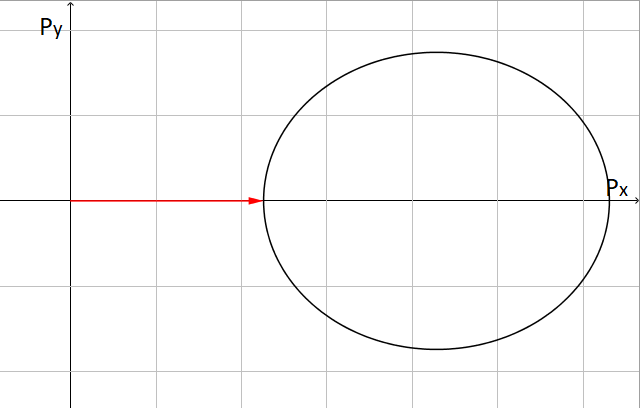
\includegraphics[scale=0.5]{1_es.png}
\end{figure}
\newpage
\begin{figure}[htbp]
\centering
\hspace{11pt}
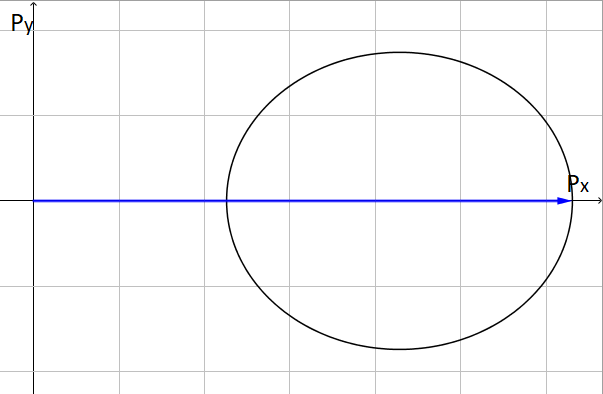
\includegraphics[scale=0.5]{2_es.png}
\end{figure}
\vspace{1em}


I casi sono quelli in cui il momento è tutto sull'asse $x$, che corrisponde ai casi di $\theta_\star = 0, \pi$, dunque con una trasformazione di Lorentz
$$ p_{MAX} = \gamma(p^\star + \beta \E^\star) = \gamma \tonde{\sqrt{\frac{M^2}{4}-m^2} + \beta \frac{M}{2}} = 1.034 \mbox{ GeV/c}$$
$$ p_{MIN} = \gamma(-p^\star + \beta \E^\star) = \gamma \tonde{-\sqrt{\frac{M^2}{4}-m^2} + \beta \frac{M}{2}} = 0.115 \mbox{ GeV/c}$$
\end{solution}

\newpage
\begin{solution}
Per comodità  di notazione denoto tutto ciò che riguarda il $\pi^-$ con apici o pedici "-", analogamente per quanto riguarda il $\pi^+$ con "+".
La seconda reazione avviene in soglia, calcolo dunque la massa equivalente $M_e$ tale da considerarla un decadimento e posso eguagliarla alla somma delle masse dei prodotti
$$ M_e^2 = P^\mu_{TOT} P_{\mu \SP TOT} = \tonde{P^\mu_p + P^\mu_-}^2 = m_p^2 + m_+^2 +2 \E_- m_p$$ 
$$ m_p^2 + m_+^2 +2 \E_- m_p = \tonde{m_\pi + m_n + m_f}^2  \Rightarrow  \E_- = \frac{\tonde{m_\pi + m_n + m_f}^2 - m_p^2 - m_+^2 }{2 m_p} = 1.8 \mbox{ GeV}$$
Per la conservazione dell'energia nella prima reazione
$$ \E_K = \frac{3}{2} \E_- = 2.7 \mbox{ GeV}  \  \Rightarrow  \  \beta_K = \frac{\sqrt{\E_K^2 - m_K^2}}{\E_K^2} = 0.9827$$
Scegliendo un sistema tale che, nel centro di massa il $\pi_-$ venga emesso a $\theta_\star$ e il $\pi_+$ a $\theta_\star - \pi$, possiamo scrivere
$$ \E_- = \gamma_K \tonde{ \E^\star + \beta_k p^\star \cos \theta^\star}$$
$$ \frac{1}{2} \E_- = \gamma_K \tonde{ \E^\star - \beta_k p^\star \cos \theta^\star}$$
Sottraendo le due equazioni ed esplicitando il coseno troviamo
$$ \cos \theta^\star = \frac{\E_-}{4 \gamma_K \beta_K p^\star} = 0.4240  \  \Rightarrow  \  \sin \theta^\star = 0.9056$$
La velocità  del $\pi_-$ nel centro di massa è invece
$$ \beta^\star_- = \frac{p^\star}{\E^\star} = 0.8 $$
Utilizzando quindi la formula 
$$ \theta_{-} = \arctan\tonde{\frac{\sin\theta_\star}{\gamma_K \tonde{ \cos \theta_\star + \frac{\beta_K}{\beta_\star^-}}}} = 5.8^\circ$$
Il $\pi_-$ percorre un arco di circonferenza con velocità  nota, poiché immerso in campo magnetico ortogonale al piano del moto
$$ \beta_- = \frac{\sqrt{\E_-^2 - m_-^2}}{\E_-^2} = 0.9965 $$
L'arco è lungo dunque $d = c \beta_- \overline{t}$. Possiamo allora trovare l'angolo sotteso all'arco
$$ \theta_{\overline{t}} = \frac{c \beta \overline{t}}{R}$$
ove il raggio è dato dalla formula
$$ R = \frac{p_- c}{e B} = 17.9 \mbox{ m}$$
La distanza, ossia il segmento che congiunge gli estremi dell'arco è
$$ L  = 2 R \sin \tonde{\theta_{\overline{t}}} = 2 \frac{p_- c}{e B} \sin \tonde{\frac{c \beta \overline{t}}{R}}$$
$$ p_- = \sqrt{\E^2_- - m^2_-} = 1.7937 \mbox{ GeV/c} $$
Per convertire in unità  di misura del sistema internazionale devo dividere per $c$, e poi tenere conto della relazione $1 \mbox{ GeV} = 1.6 \cdot 10^{-10} \mbox{ J}$. 
$$ p_- = \frac{1.7937}{3 \cdot 10^8 } \times 1.6 \cdot 10^{-10}=  9.57 \cdot 10^{-19} \mbox{ kg}\cdot \mbox{m} \cdot \mbox{s}^{-1} $$
Da cui segue $L = 0.1 \mbox{ m}$.
\end{solution}


\begin{solution}
Il problema mi pare sia da interpretare nel seguente modo: supponiamo di avere in un sistema un campo elettromagnetico uniforme e costante e tale che $\vec E \cdot \vec B = 0$ e $B^2 - E^2 = 0$. Allora sappiamo che esiste un sistema di riferimento $\mathcal{S}'$ tale che ci sia solo campo magnetico. Si potrebbe porre il problema esattamente in questa maniera, e semplicemente dire che il campo magnetico in $\mathcal{S}'$ è generato da un magnete. Allora si vede subito l'analogia del fatto che la velocità  del magnete è la velocità  del boost da fare un caso generale. Quindi definisco ora il sistema $\mathcal{S}$ quello in cui è presente il campo elettromagnetico, e ha senso dunque che vari l'energia del fascio di protoni. Definisco invece $\mathcal{S}'$ il sistema solidale al magnete in movimento. Allora in $\mathcal{S}'$ sappiamo che $\vec{B}' = (0,0,\sqrt{2} \cdot 10^9 \mbox{ V/m})$, e inoltre
$$ B' = \gamma \tonde{ B - \beta E'} = \frac{E}{\gamma \beta}$$
L'estensione in direzione $y \parallel y'$ non cambia nei due sistemi di riferimento ed è sempre $L$. Allora per la legge di potenza in $\mathcal{S}$
$$ \Delta \E = \E - \E_0 = e E L = \gamma \beta e B' L  \  \Rightarrow  \  \beta = \frac{\Delta \E}{\sqrt{\Delta \E^2 + \tonde{e B' L}^2}} = \frac{1}{3}$$
L'urto è elastico, dunque la reazione che avviene è 
$$ p^+ + \pi^+ \longrightarrow p^+ + \pi^+ $$
Calcolo la massa equivalente $M_e$ tale da considerare l'urto come un decadimento e utilizzare le solite formule
$$ M_e^2 = (P^\mu_{TOT} P_{\mu \SP TOT}) = M^2 + 2 \E m + m^2  \  \Rightarrow  \  M_e = 1.5999 \mbox{ GeV/c}^2$$
Dunque il centro di massa si muove alla velocità 
$$ \beta_c = \frac{\modulo{p}}{\E + m} = \frac{\sqrt{\E^2-M^2}}{\E-m} = 0.9589 $$
Calcoliamo l'energia e il momento dei protoni nel centro di massa
$$ \E^\star_p = \frac{M_e^2 + M^2 - m^2}{2M_e}  \  \modulo{p}^\star_p = \sqrt{\frac{M_e^4 + M^2 + m^2 - 2M^2 m^2 - 2(M^2 + m^2)M^2_e}{4M^2}}$$
Dunque $p^\star_p = 0.4732$ GeV/c, mentre $\E^\star_p = 1.1063$ GeV.
Dunque la velocità  dei protoni nel centro di massa, dopo l'urto, è
$$ \beta_p^\star = \frac{\sqrt{M_e^4 + M^4 + m^4 - 2M^2 m^2 - 2(M^2 + m^2)M^2_e}}{M_e^2 + M^2 - m^2}  = 0.4278 $$
Quindi 
$$ \theta_{MAX} = \arcsin \tonde{ \frac{p^\star_p}{M \beta_c \gamma_c}} \overset{calcoli/Barone}{=} \arcsin \tonde{\frac{m}{M}}=8.05^\circ$$
Dalla formula [7.127] del Barone
\begin{eqnarray*} 
\E'_p & = & \frac{(\E + m)(M^2 + m \E) + p_p^2 \cos \theta_{MAX} \sqrt{m^2 - M^2 \sin^2 \theta_{MAX}}}{(\E + m)^2 - p^2_p \cos^2 \theta_{MAX}} \\
& = & \frac{(\E + m)(M^2 + m \E)}{(\E + m)^2 - (\E^2 - M^2) \tonde{1 - \frac{m^2}{M^2}}} = 3.18 \mbox{ GeV}
\end{eqnarray*}
\end{solution}

\newpage
\begin{solution}
Siccome gli $e$ collidono frontalmente, ossia con angolo $\alpha = \pi$, allo stesso modo avverrà  nel centro di massa, poiché facendo un boost lungo quella direzione, giacendo sulla stessa retta, i momenti non cambiano direzione. Dal fatto inoltre che nel centro di massa il momento totale è nullo, capiamo che $ p^\star_- = - p^\star_+$, e dunque anche le energie sono uguali per via della stessa massa. I "minimi requisiti" per cui possa avvenire la reazione è che essa avvenga in soglia, ossia che i prodotti siano fermi nel centro di massa. Allora per la conservazione del quadri-momento, totale, prima e dopo l'urto
$$ \tonde{2 \E^\star_e,0,0,0} = \tonde{2 M,0,0,0}  \  \Rightarrow  \  
\E^\star_e = M  \  \Rightarrow  \  p^\star_+ = \sqrt{M^2 -m^2} $$
Allora con una trasformazione di Lorentz torniamo nel laboratorio, denotando $\beta$ con la velocità  del centro di massa
$$ p^+ = \gamma \tonde{ p^\star_+ + \beta \E^\star_e}  \  
\E^+ = \gamma \tonde{ \E^\star_e + \beta p^\star_+  } $$
Possiamo da qui ricavare la velocità  dei positroni, che era nota
$$ \beta_+ = \frac{p_+}{\sqrt{p_+^2 + m^2}} = \frac{ p^\star_+ + \beta \E^\star_e}{ \E^\star_e + \beta p^\star_+  }  \  \Rightarrow  \  
\beta = \frac{ p^\star_+ - \beta_+ \E^\star_e}{ - \E^\star_e + \beta_+ p^\star_+  }$$
Dunque 
$$ \beta = \frac{ \sqrt{M^2 -m^2} - M \frac{p_+}{\sqrt{p_+^2 +m^2}} }{\frac{p_+}{\sqrt{p_+^2 +m^2}} \sqrt{M^2 -m^2} - M } = -0.9810 $$
Potrebbe turbare il fatto che sia trovato un segno negativo. In realtà , ciò vuol dire che se scegliamo come verso positivo il verso in cui viaggia il fascio di positroni, allora il centro di massa viaggia nel verso opposto. Questo significa che gli elettroni sono più veloci dei positroni e hanno dunque un modulo del momento più alto. Ciò torna poiché gli elettroni/positroni hanno massa praticamente trascurabile rispetto ai loro prodotti, perciò devono avere alta energia per produrre qualcosa di così più massivo, e notato che anche $p^+$ non è esagerato, è normale aver l'indicazione che il $p^-$ dev'essere tanto più alto.
\\
Troviamo il $p_-$
$$ p_- = \gamma \tonde{ - p^\star_+ + \beta \E^\star_+} = \gamma \tonde{ - \sqrt{M^2- m^2 } + \beta M} =  - 1021.09 \mbox{ MeV/c}$$
Come aspettato, il $p^-$ è decisamente più alto.
\\
Supponiamo d'ora in poi quindi $p_- = - 2042.17 $ MeV/c. Calcoliamo la massa equivalente dell'urto al fine da considerarlo un decadimento
$$ M^2_e = \tonde{P^\mu_+ + P^\mu_-}^2 = 2m^2 + 2 \E_+ \E_- - 2 p^+ p_- \cos \alpha =  2m^2 + 2 \E_+ \E_- + 2 p^+ p_- $$
E facendo i conti troviamo $M_e = 286.00 $ MeV/c$^2$. Allora ora possiamo ricavare la velocità  dei muoni nel centro di massa
$$ \beta^\star_\mu = \frac{p^\star_\mu}{\E^\star_\mu} = \sqrt{1 - \frac{4M^2}{M^2_e}} = 0.7148$$
In questo caso la velocità  del centro di massa è invece
$$ \beta = \frac{p_+ + p_-}{E_+ + E_-} = 0.999994 $$
Sicuramente allora esiste l'angolo massimo, che sarà 
$$ \theta_{MAX} = \arcsin \tonde{ \frac{p^\star}{M \beta \gamma}} = \arcsin \tonde{ \frac{1}{M \beta \gamma} \sqrt{\frac{M^2_e}{4} - M^2}} =  0.2^\circ$$
\end{solution}

\begin{solution}
L'angolo massimo ci fornisce una relazione tra $p_\pi$ e dati noti. Infatti, denotanto $\beta$ la velocità  dei $\pi$, e quindi del centro di massa
$$ \sin\overline{\theta} = \frac{p^\star_\mu}{ m \beta \gamma} = \frac{ M p^\star_\mu}{ m p_\pi}  \  \Rightarrow  \  p_\pi = \frac{ M p^\star_\mu}{ m \sin\overline{\theta}} = 
 \frac{ (M^2 - m^2) }{ 2 m \sin\overline{\theta}} = 1949.79 \mbox{ MeV}$$
Inoltre sappiamo che, all'angolo massimo nel laboratorio, il coseno dell'angolo nel centro di massa è
$$ \cos \theta^\star = - \frac{\beta^\star_\mu}{\beta} = 73.70^\circ$$
Dove
$$ \beta = \frac{p_\pi}{\E_\pi} = 0.9974  \  \beta^\star_\mu =
\frac{p^\star_\mu}{\E^\star_\mu} = \frac{M^2 -m^2}{M^2 + m^2} = 0.2800 $$
Allora possiamo trovare l'energia nel laboratorio
$$ \E_\mu = \gamma \tonde{ \E_\mu^\star  + \beta p^\star_\mu \cos \theta^\star } = \gamma \frac{2 M m^2}{ (M^2 + m^2)} = 1398.75 \mbox{ MeV}$$
L'energia massima che $\mu$ può avere nel laboratorio è invece
$$\E_\mu = \gamma \tonde{\E_\mu^\star + \beta p_\mu^\star} = \gamma \frac{M^2 + m^2 + \beta(M^2 -m^2)}{2M} = 1941.61 \mbox{ MeV}$$
In questa situazione l'angolo nel centro di massa è $\theta^\star =0$ e altro non può essere anche nel laboratorio, dunque $\theta = 0$. 
\\
Suppongo che il $\tau$ fornito dal testo sia il tempo di vita media nel sistema proprio dei muoni. Il tempo di vita media nel laboratorio è invece
$$ \tau_L = \frac{d}{c \beta_\mu}  \  \Rightarrow  \  \tau = \frac{d}{c \gamma_\mu  \beta_\mu} = \frac{d  m}{c p_\mu}  \  \Rightarrow  \  d  = \frac{\tau c p_\mu}{m} = \tau c \sqrt{\frac{\E_\mu^2}{m^2} - 1} = 12.2 \mbox{ km}
$$
La densità  di probabilità  di energia è costante, e vale dunque
$$ \rho (\E) = \frac{1}{2  \gamma \beta p^\star_\mu} = \frac{Mm}{ p_\pi (M^2 - m^2) }$$
Allora la probabilità 
$$ P (1300 \leq \E_\mu \leq 1600) = \frac{Mm(1600-1300)}{ p_\pi (M^2 - m^2) } = 26.4 \% $$
\end{solution}



\begin{solution}
Il $K$ è prodotto ad angolo nullo nel laboratorio, di conseguenza lo è anche nel centro di massa. Calcoliamo la velocità  del centro di massa 
$$ \beta_{CM} = \frac{p_{CM}}{\E_{CM}} = \frac{\E_\gamma}{ \E_\gamma + m_\phi} = 0.2000$$
Calcoliamo la massa equivalente dell'urto
$$ M_e^2 = (P^\mu_\gamma + P^\mu_\phi)^2 = m^2_\phi + 2\E_\gamma m_\phi = 1.5 \mbox{ GeV}^2 \mbox{/c}^4$$
Allora 
$$ \E_K = \gamma_{CM} (\E_K^\star + \beta_{CM} p_K^\star) = \gamma_{CM} \tonde{\frac{\sqrt{m^2_\phi + 2\E_\gamma m_\phi}}{2} + \beta_{CM} \sqrt{ \frac{m^2_\phi + 2\E_\gamma m_\phi}{4} -m_K^2}}$$
E la formula porge $\E_K = 697.17 $ MeV. Dunque
$$ \beta_K = \frac{\sqrt{\E_K^2 - m_K^2}}{\E_K} = 0.6969$$
Occorre ora trovare la velocità  della $\pi$ nel centro di massa 
$$ \beta_\pi^\star = \sqrt{1 - 4\frac{m^2_\pi}{m^2_K}} = 0.8000$$
Siamo nel caso $\gamma_{K} \beta_{K} > \beta_\star^\pi > \beta_K$. Allora l'angolo minimo è
$$ \theta_{MIN} = 2 \arctan \tonde{\frac{\beta^\star_\pi}{\beta_{K} \gamma_{K}}} = 78.9^\circ$$
L'angolo che i prodotti formano con la linea di volo del $K$ nel centro di massa, corrispondente all'angolo minimo, è pari a $\frac{\pi}{2}$ e dunque c'è simmetria. Allo stesso modo facendo un boost, le particelle hanno massa uguale, quindi non c'è motivo perché il boost agisca in modo "diverso" rompendo la simmetria. Allora da qui si capisce che le particelle hanno momento ed energia uguali. Per questo motivo allora hanno anche i raggi delle eliche uguali poiché dipendono soltanto dall'intensità  del campo e dalla componente del momento perpendicolare ad esso. Dunque
$$ R = \frac{c p_\pi \sin \frac{\pi}{6}}{ e B} = \frac{c p_\pi}{2 e B} $$ 
$$ \E_\pi = \gamma_K \E_\pi^\star = \gamma_K \frac{m_K}{2} = 348.59 \mbox{ MeV}  \  \Rightarrow  \  p_\pi = 314.67 \mbox{ MeV/c}$$
Se utilizziamo il momento in eV, allora possiamo porre la carica del pione pari a $1$, poiché ha la stessa carica del protone. Allora dobbiamo dividere per un $c$, poiché il momento è ancora in unità  di $\frac{1}{c}$
$$ R = \frac{3 \cdot 10^8 \times 3.1467 \cdot 10^8 }{2 \cdot 10^9 \times 3 \cdot 10^8} =15.73 \mbox{ cm}$$
\end{solution}

\begin{solution}
L'energia minima a cui avviene la reazione è la situazione in cui i $\pi$ sono prodotti in soglia. Uguagliamo il quadrimomento nel centro di massa, prima e dopo l'urto, sfruttando la condizione di soglia
$$ (2 \E^\star_\mu,0,0,0) = (2 m_\pi,0,0,0 )  \  \Rightarrow  \  \E^\star_\mu = m_\pi  \  p_\mu^\star = \sqrt{m^2_\pi - m^2_\mu} $$
Ora sfruttando una trasformazione di Lorentz, e scegliendo i $\mu^-$ che viaggiano in verso positivo
$$ \E_0 = \gamma_{CM} \tonde{\E^\star_\mu +\beta_{CM} p^\star_\mu} $$
$$ \frac{\E_0}{2} = \gamma_{CM} \tonde{\E^\star_\mu - \beta_{CM} p^\star_\mu} $$
Si può trovare la velocità  del centro di massa
$$\beta_{CM} =  \frac{\E^\star_\mu}{3 p^\star_\mu} =  \frac{m_\pi}{3 \sqrt{m^2_\pi - m^2_\mu}}$$
Sostituendo nella prima equazione troviamo l'energia minima
$$\E_0 = 4 m_\pi \sqrt{\frac{m^2_\pi - m^2_\mu}{8 m^2_\pi - 9m^2_\mu}}= 223.60 \mbox{ MeV}$$
Adesso per il secondo punto assumo che l'energia $\E \geq \E_0$. Scelgo la direzione $x$ quella in cui è diretto il boost con velocità  $\beta$, e la direzione su cui si scontrano i muoni è inclinata di $\alpha$ rispetto all'asse $x$. Scelgo ancora che i $\mu^-$ viaggino in direzione positiva, quindi
$$ \E' = \gamma \tonde{\E - \beta p_- \cos \alpha} $$
$$ \E' = \gamma \tonde{\frac{\E}{2} + \beta p_+ \cos \alpha} $$
Dunque
$$ \E - \beta p_- \cos \alpha = \frac{\E}{2} + \beta p_+ \cos \alpha  \  \Rightarrow  \  \beta = \frac{\E}{2 (p_+ + p_- ) \cos \alpha} $$
In condizioni di energia minima i pioni prodotti hanno ugual energia e modulo del momento nel laboratorio. Dunque i raggi delle orbite sotto l'effetto del campo magnetico sono gli stessi. Con una trasformazione di Lorentz troviamo l'energia dei pioni nel laboratorio
$$ \E_\pi = \gamma_{CM} \E^\star_\pi = \gamma_{CM} m_\pi = 3 m_\pi \sqrt{\frac{m_\pi^2 - m_\mu^2}{8 m_\pi^2 - 9 m_\mu^2}}$$
Dunque il raggio è (opportunamente dividendo per $c$ il momento perché è ancora in unità  di $1$/$c$) 
$$ R = \frac{c p_\pi}{e B} = \frac{c \frac{3 m_\pi}{c} \sqrt{\frac{m_\pi^2 - m_\mu^2}{8 m_\pi^2 - 9 m_\mu^2} - m_\pi^2}}{e B} = \frac{m_\pi^2}{eB} \sqrt{\frac{1}{8m^2_\pi -9 m^2_\mu} } = 7.5 \mbox{ m}$$
N.B. Ricordarsi di esprimere il momento in eV così da considerare la carica dell'elettrone pari ad $1$.
\\
La forma delle traiettorie in $\mathcal{S}$ è chiara, sono delle orbite circolari. Nei sistemi $\mathcal{S}'$, visto che effettuiamo un boost, comparirà  anche un campo elettrico che, dato che esiste $\mathcal{S}$, sarà  ortogonale alla direzione del boost e del campo magnetico (sia vecchio che nuovo) e tale che $B'^2 - E'^2 > 0$. Allora qui la traiettoria sarà  un'ellisse, ossia un cerchio schiacciato.
\end{solution}

\newpage
\renewcommand{\theindexsol}{$\Q$}
\subsection{Corpo nero}
\begin{solution}
	Per calcolare teoricamente la costante di Stefan-Boltzmann, $ \sigma_{\mathrm{S.-B.}}$ , si considera che la densità di energia di un gas che viene scaldato ad una certa temperatura segue la seguente relazione: \begin{equation*}
        u (\nu , T) = \frac{8 \pi}{c^3} \ \frac{h \nu^3}{e^{\frac{h \nu}{K_B T}}- 1}    
        \end{equation*}
        
        Se si pone $\frac{h \nu}{K_B T} = x $ \ e \ $\frac{h }{K_B T} \ d\nu = dx$ si ottiene l'integrale: \begin{equation*}
        u(T) = \frac{8 \pi}{c^3} \ h \ \int_{0}^{\infty} {\frac{\nu^3}{e^{\frac{h \nu}{K_B T}}- 1}} \ d\nu = \frac{8 \pi}{c^3} \ h \ \left( \frac{K_B T}{h}\right)^4 \ \int_{0}^{\infty} {\frac{x^3}{e^x - 1 }} \ dx = \frac{8 \pi^5}{c^3} \ \frac{K^4_B T^4}{15 h^3}  
        \end{equation*}
        
        \bigskip
        Sapendo che $I =  \sigma_{\mathrm{S.-B.}} T^4$ si ha che: \begin{equation*}
        I = \frac{1}{4} u c = \frac{2 \pi^5 K_B^4 T^4}{15 \ c^2 h^3 } =  \sigma_{\mathrm{S.-B.}} T^4  \  \Rightarrow  \    \sigma_{\mathrm{S.-B.}} = \frac{2 \pi^5 K_B^4 }{15 \ c^2 h^3 } = 5.66 \cdot 10^{-8} \ \frac{\mathrm{W}}{\mathrm{m}^2 \mathrm{K}^4} 
        \end{equation*}
\end{solution}

\stepcounter{solution}
\begin{solution}
	\textbf{N.B.} in questo problema sembra esserci un errore relativo al valore della lunghezza d'onda, che dovrebbe essere $\lambda_{\mathrm{max}} = 1.5 \cdot 10^{-6} \ \mathrm{m}$ .

\medskip
a. \ Per calcolare il valore della temperatura si applica la legge di Wien per cui: \begin{equation*}
 T = \frac{\lambda_{\mathrm{Wien}}}{\lambda_{\mathrm{max}}} = \frac{2.897 \cdot 10^{-3}}{1.5 \cdot 10^{-6}} = 1931 \ \mathrm{K}  
\end{equation*}

\bigskip
b. \ Tra l'intensità $I$, misurata a distanza $l$ dal corpo nero,  e l'intensità $I_c$ che viene misurata sulla superficie del corpo nero vi è una relazione dovuta alla conservazione dell'energia:  \begin{equation*}
 I_s = \sigma_{\mathrm{Stefan-Boltzman} } T^4 = \frac{P_0}{ 4\pi R^2} = \frac{I \ 4\pi l^2}{4 \pi R^2} = \frac{I \ l^2}{R^2}  \  \Rightarrow  \  R = 0.01 \ \mathrm{m}  
\end{equation*}

\bigskip
c. \ $P = I_s \ 4\pi R^2 = \sigma_{\mathrm{Stefan-Boltzman} } T^4 \ 4\pi R^2 = 995 \ \mathrm{W}$

\bigskip
d. \ Essendo una cavità sferica e radiazione non collimata si considera che l'intensità è uguale a \ $I = \frac{1}{4} u c $ \ dunque la densità di energia sarà uguale a \ $u = \frac{4 \ I}{c} = 0.0104 \ \frac{\mathrm{J}}{\mathrm{m}^2} $ 
\end{solution}

\newpage
\begin{solution}
	Applicando la Legge di Wien per cui  \ $\lambda_\mathrm{MAX}  T = \lambda_{\mathrm{Wien}} = 2.897 \cdot 10^{-3} \ {\mathrm{K \ m}}$ ,  si ottiene: 
 \begin{equation*}
     T_s = \frac{\lambda_{\mathrm{Wien}}}{\lambda_{\mathrm{MAX}}} = 5794 \ \mathrm{K} 
 \end{equation*}
\end{solution}


\begin{solution}
	Le intensità totali del Sole e della Terra sono: $I_S = \sigma  T^4_S$ \ ; \ $I_T = \sigma  T^4_T$ 
  mentre le potenze emesse sono $W_S = 4\pi \ r^2_S \ \sigma T^4_S$ \ ;  $W_T = 4\pi \ r^2_T \ \sigma T^4_T$ 
 
 \medskip
 Essendo corpi neri ciò che assorbono viene emesso idealmente. Si può perciò pensare che ${W}_T = {W}_{S,T} = I_{S,T} \ \pi r^2_t$ con $I_{S,T} = \frac{W_S}{4\pi d^2}$, ovvero l'intensità del Sole che si misura dalla Terra. 
 Considerando la geometria del problema si ha che $\frac{D}{2d} = \tg{\frac{\theta}{2}} \sim \frac{\theta}{2}$ per cui: 
 \begin{equation*}
     W_T = W_{S,T}  \  \Rightarrow  \  4\pi r^2_t \ \sigma \ T^4_T = \frac{4\pi \ r^2_S \ \sigma T^4_S}{4\pi d^2} \ \pi r^2_t   \  \Rightarrow  \  T_S = T_T \ \sqrt[4]{\frac{16}{{\theta}^2}}  = 6011 \ \mathrm{K} 
 \end{equation*}
\end{solution}



\begin{solution}
 In questo caso considerando la risoluzione del problema precedente basta invertire l'ultima relazione tra le temperature per ottenere $T_M$: 
 \begin{equation*}
     T_M = T_S \ \sqrt[4]{\frac{\theta^2}{16}} = 234 \ \mathrm{K} 
 \end{equation*}
\end{solution}



\begin{solution}
 \begin{equation*}
 L = 4\pi r^2_S \ I_S = 4\pi r^2_S \ \sigma \ T^4  \  \Rightarrow  \  r_S = \sqrt{\frac{L}{4\pi \ \sigma \ T^4_s}} = 6.45 \cdot 10^8 \ \mathrm{m}  
 \end{equation*}
\end{solution}


\newpage
\begin{solution}
 Con $ L_s = 4\pi r^2_S \ \sigma \ T^4 $ ,  $ L_G = 4\pi r^2_G \ \sigma \ T^4 $ si ottiene: 
 \begin{equation*}
     \frac{r_G}{r_S} = \sqrt{\frac{100 \ T^2_S}{T^2_G}} = 40 
 \end{equation*}
\end{solution}



\begin{solution}
\begin{enumerate}[label=(\textit{\roman*})]
	\item Tenendo a mente la relazione $E = P \ dt = dm c^2$ , si ottiene: 
\begin{equation*}
    \frac{dm}{dt} = \frac{P}{c^2} = \frac{4\pi r^2_S \ \sigma T^4_S}{c^2} = 5.03 \cdot 10^9 \ \mathrm{Kg} 
\end{equation*}

\item \begin{equation*}
    \Delta t = \frac{1\% \ m_S}{5.03 \cdot 10^9} = 3.98 \cdot 10^{18} \ \mathrm{s} 
\end{equation*}
\end{enumerate}
\end{solution}



\begin{solution}
	 Secondo il modello di Rayleigh-Jeans, che porta alla catastrofe ultravioletta, è possibile calcolare il numero di modi di vibrazione come $N(\nu) = \frac{8\pi}{c^3} \ V \ \nu^2 d\nu$. Dunque si può misurare il numero di modi di vibrazione per unità di volume, teendo a mente la relazione $\nu = \frac{c}{\lambda}$, come: \begin{equation*}
  dn = \frac{dN}{dV} = \frac{8\pi}{c^3} \ \nu^2 \ d\nu =  \frac{8\pi}{c^3} \ \frac{c^2}{\lambda^2} \frac{c}{\lambda^2} \ d\lambda   
 \end{equation*}
 Integrando l'ultima espressione si trova $n$: \begin{equation*}
     \int dn = \int_{4.990}^{5.010} \frac{8\pi}{c^3} \ \frac{c^2}{\lambda^2} \frac{c}{\lambda^2} \ d\lambda = \frac{8\pi}{3} \left[- \frac{1}{\lambda^3}\right] = 8.04 \cdot 10^{26} \ \mathrm{modi/m}^3 
 \end{equation*}
\end{solution}


\newpage
\begin{solution}
	 Considerando che l'intensità di un corpo nero con radiazione non collimata si ottiene come $I = \frac{1}{4} \ u c$ si può considerare la variazione dell'intensità in questo caso applicando la formula di Planck per la densità di energia: \begin{equation*}
     dI = \frac{1}{4} \ c \ \frac{8\pi \ h \nu^3}{c^3} \ \frac{1}{e^{\frac{hc}{KT}}-1} = \frac{2\pi \ c^2h}{\lambda^5 \ (e^{\frac{hc}{\lambda KT}}-1)} \ d\lambda     
 \end{equation*}
 La potenzia misurata è dunque: \begin{equation*}
     P = \int_{0.4}^{0.7} dI(\lambda) = \frac{d^2 \pi^2 c^2 h}{2 \overline{\lambda}^5 \ (e^{\frac{hc}{\overline{\lambda} KT}} -1)} \ (0.7-0.4) \cdot 10^{-6} = 63 \ \mathrm{W} 
 \end{equation*}
\end{solution}



\newpage
\subsection{Effetto fotoelettrico, fotoni e raggi X}
\begin{solution}
	Sapendo che per effetto fotoelettrico un fotone ha energia \ $\mathcal{E} = h \nu = 6.626 \cdot 10^{-34} \ \nu  $ \  e che la relazione tra energia e potenza è $\mathcal{E} = P \cdot t$ \ si ottiene: \begin{equation*}
    \frac{\mathrm{\#fotoni}}{\mathrm{s}} = \frac{P}{\mathcal{E}} = \frac{10^3}{6.626 \cdot 10^{-34} \ 880 \cdot 10^{3}} = 1.72 \cdot 10^{30} 
\end{equation*}
\end{solution}




\begin{solution}
\begin{enumerate}[label=(\textit{\roman*})]
	\item Per ottenere il numero di fotoni è necessario conoscere la potenza data dall'intensità che arriva sulla Terra: \begin{equation*}
    P_t = I_t \ 1 \ \mathrm{m}^2 = 1.4 \cdot 10^3 \ \mathrm{W}  \  \Rightarrow  \  \frac{\mathrm{\#fotoni}}{\mathrm{s}} = \frac{P}{\mathcal{E}} = \frac{1.4 \cdot 10^3}{6.626 \cdot 10^{-34} \ 5 \cdot 10^{14}} = 4.23 \cdot 10^{21} 
\end{equation*}

\item La potenza del Sole si ottiene come: \begin{equation*}
    P_s = I_t \ 4\pi d^2 = 3.96 \cdot 10^{26} \ \mathrm{W}  \  \Rightarrow  \  \frac{\mathrm{\#fotoni}}{\mathrm{s}} = \frac{P}{\mathcal{E}} = \frac{3.96 \cdot 10^{26}}{6.626 \cdot 10^{-34} \ 5 \cdot 10^{14}} = 1.2 \cdot 10^{45} 
\end{equation*}

\item Si considera che la radiazione è collimata per cui $I = u c $ \ . Questo porta ad avere un numero di fotoni per metro cubo pari a: \begin{equation*}
 \frac{\mathrm{\#fotoni}}{\mathrm{s}} = \frac{P}{\mathcal{E} c} = \frac{1.4 \cdot 10^{3}}{6.626 \cdot 10^{-34} \ 5 \cdot 10^{14} \ 3 \cdot 10^{8}} = 1.42 \cdot 10^{13}   
\end{equation*}
\end{enumerate}
\end{solution}




\begin{solution}
\begin{enumerate}[label=(\textit{\roman*})]
	\item Il potenziale di estrazione che si stima è: $\Phi_0 = h \nu_0 = 6.626 \cdot 10^{-34} \ 1.10 \cdot 10^{15} = 7.29 \cdot 10^{-19} \ \mathrm{J} = 4.5 \ \mathrm{eV}$
	\item L'energia massima degli elettroni estratti corrisponderebbe all'energia cinetica che hanno acquisito pari a: 
\begin{gather} 
    K_{\mathrm{max}} = \mathcal{E}_{\mathrm{max}} - \  \Phi_0 = h (\nu - \nu_0) = 6.626 \cdot 10^{-34} \ (1.50 - 1.10 ) \cdot 10^{15} \\= (9.939 - 7.29) \cdot 10^{-19} \ \mathrm{J} = (6.2 - 4.5) \ \mathrm{eV} = 1.7 \ \mathrm{eV} 
\end{gather}

\item La corrente estratta dall'elettrodo è uguale a \ $I = \frac{\Delta q }{\Delta t} = \frac{(1/100) \ \mathrm{fotoni} \cdot e}{\Delta t}$ \ . Si calcolano, dunque, i fotoni per secondo emessi dalla radiazione: 
\begin{equation*}
 \frac{\mathrm{\#fotoni}}{s} = \frac{P}{\mathcal{E}} = \frac{I \ S}{h \nu} = \frac{10^{-4} \ 24}{6.626 \cdot 10^{-34} \ 1.5 \cdot 10^{15}} = 2.52 \cdot 10^{15}  \  \Rightarrow  \  \frac{1}{100} \ \mathrm{fotoni} = 2.52 \cdot 10^{13}  
\end{equation*}

In conclusione: \begin{equation*}
 I = \frac{(1/100) \ \mathrm{fotoni} \cdot e}{\Delta t} = 4.02 \ \mu \mathrm{A}   
\end{equation*}
\end{enumerate}

\end{solution}





\begin{solution}
\begin{enumerate}[label=(\textit{\roman*})]
	\item La frequenza massima stimata è pari a: \begin{equation*}
\nu_{\mathrm{max}} = \frac{\Delta V}{h} = \frac{10^4}{4.136 \cdot 10^{-15}} = 2.42 \cdot 10^{18} \ \mathrm{Hz}  
\end{equation*}

\item Con $\Delta V_1 = 50 \ \mathrm{kV}$ \ : 

\begin{equation*}
 \lambda_{\mathrm{min}} = \frac{h c}{\Delta V_1} = 2.49 \cdot 10^{-11} \ \mathrm{m}   
\end{equation*}

\end{enumerate}
\end{solution}



\begin{solution}
	Per effetto fotoelettrico si ha che $E = \phi$ , quindi bisogna trovare l'energia in funzione di $I$ e $\sigma$.
 \begin{equation*}
    E = P \tau = \frac{I}{\sigma} \ \tau = \frac{2 \cdot 10^{-2} \ \mathrm{W/m}^2}{ 3\cdot 10^{19} \ \mathrm{e/m}^2} = \frac{2 \cdot 10^{-2}}{3 \cdot 10^{19} \cdot 1.62 \cdot 10^{-19}} = \phi  
 \end{equation*}
 
 quindi \begin{equation*}
     \tau = \frac{\phi}{P} = \frac{4.73 \cdot 3 \cdot 1.62}{2 \cdot 10^{-2}} = 1149.9 \ \mathrm{s} 
 \end{equation*}
\end{solution}


\newpage
\begin{solution}
	\begin{equation*}
     \phi = h \nu_{\mathrm{min}} = \frac{hc}{\lambda_{\mathrm{max}}} = 4.07 \ \mathrm{eV} 
 \end{equation*}
\end{solution}



\begin{solution}
	Il potenziale di arresto $V_0$ non è altro che l'energia cinetica massima che per effetto fotoelettrico è legata al potenziale di estrazione, $\phi$, e all'energia dell'onda incidente, $h\nu$, tramite la relazione: \ $h\nu = \phi + V_0$ . Quindi: \begin{equation*}
     V_0 = \frac{hc}{\lambda} - \phi = 0.44 \ \mathrm{eV} 
 \end{equation*}
\end{solution}


\newpage
\subsection{Modello di Bohr}
\begin{solution}

\begin{enumerate}[label=(\textit{\roman*})]
	\item \ Dalla relazione $\mathcal{E}_n = - \frac{Z^2}{n^2} \ \mathcal{E}_0$ si ottiene il numero quantico: \begin{equation*}
n = \sqrt{\frac{- Z^2 \ \mathcal{E}_0}{\mathcal{E}_n}} = 4    
\end{equation*}

\item La velocità degli elettroni si ottiene partendo dal momento angolare $L = n \hbar = r_n \ m \ v_n$  e dalla relazione tra la forza di Coulomb e la forza centripeta: 

 \begin{equation*}
\begin{cases}
    \frac{Z e^2}{4\pi \epsilon_0 \ r^2_n} = m v^2_n r_n  \  \Rightarrow  \  r_n = \frac{16 \hbar \ 4\pi \epsilon_0 }{Z e^2 m} \\
    \\
    v_n = \frac{n \hbar}{r_n m }  \  \Rightarrow  \  v_n = \frac{Z e}{16 \pi \epsilon_0 \ 6.582 \cdot 10^{-16}} = 1.09 \cdot 10^{6} \ \mathrm{m/s}\\
\end{cases}    
\end{equation*}

\item La massima lunghezza dell'onda emessa nello spettro di emissione corrisponde al caso in cui si ha contemporaneamente la minima frequenza. Questo avviene quando l'elettrone passa dal livello $n = 4$ al livello $n =3$: \begin{equation*}
 \lambda_{\mathrm{max}} = \frac{h c}{\mathcal{E}_{4 \rightarrow 3}} = \frac{h c }{Z^2 \ \mathcal{E}_0} \ \left(\frac{1}{9} - \frac{1}{16}\right)^{-1} = 496  \ \mathrm{nm}   
\end{equation*}

\item Per simmetria si ottiene la minima lunghezza d'onda nel caso in cui si passa dal livello energetico $n = 4$ \ a \ $n = 1$: \begin{equation*}
 \lambda_{\mathrm{min}} = \frac{h c}{\mathcal{E}_{4\rightarrow 1}} = \frac{h c }{Z^2 \ \mathcal{E}_0} \ \left(1 - \frac{1}{16}\right)^{-1} = 24.3  \ \mathrm{nm}   
\end{equation*}

\item L'energia necessaria per strappare l'elettrone agli atomi eccitati si ottiene come \ $\mathcal{E} = h \nu_{\mathrm{min}} = \frac{h c }{\lambda_{\mathrm{max}}} = 2.5 \ \mathrm{eV}$ 
\end{enumerate}
\end{solution}

\newpage
\begin{solution}

\begin{enumerate}[label=(\textit{\roman*})]
	\item Tenendo conto della relazione tra l'energia si ottiene:
\begin{equation*}\begin{cases}
 \mathcal{E}_n = - \frac{Z^2}{n^2} \ \mathcal{E}_0  \   \Rightarrow  \  n^2 = - \frac{Z^2}{\mathcal{E}_n} \ \mathcal{E}_0 \\ 
 \\
 \frac{h c }{\lambda_{min}} = \mathcal{E}_{4\rightarrow 1} = - Z^2 \ \mathcal{E}_0 \ \left(1 - \frac{1}{n^2}\right)  \  \Rightarrow  \   Z = 3  \\
 \end{cases} 
\end{equation*}

\item $n = \sqrt{\frac{- Z^2 \ \mathcal{E}_0}{\mathcal{E}}} = 4$
\item $\lambda_{\mathrm{max}} = \frac{h c}{\mathcal{E}_{4 \rightarrow 3}} = \frac{h c}{Z^2 \ \mathcal{E}_0} \ \left(\frac{1}{9} - \frac{1}{16}\right) = 209 \ \mathrm{nm}$

\item La massima lunghezza d'onda che si ottiene per estrarre un elettrone eccitato agli ioni si ottiene considerando l'energia allo stato massimo di eccitazione: 
\begin{equation*}
 \lambda'_{\mathrm{max}} = \frac{h c }{\mathcal{E}_4} = 162  \ \mathrm{nm}  
\end{equation*}
\end{enumerate}
\end{solution}




\begin{solution}
\vspace{-20pt}
\begin{enumerate}[label=(\textit{\roman*})]
	\item Il minimo potenziale di accelerazione al quale il gas comincia a emettere luce si ottiene considerando la variazione dell'energia dal primo livello energetico al secondo: \begin{equation*}
V_0 = \Delta \mathcal{E} = \mathcal{E}_2 - \mathcal{E}_1 = \frac{- Z^2 \mathcal{E}_0}{n^2} - (-  13.6) =  \frac{- \mathcal{E}_0}{4} + 13.6 = 10.2 \ \mathrm{eV}  
\end{equation*}

\item La lunghezza d'onda emessa è pari a: \begin{equation*}
\lambda = \frac{h c }{V_0} = 121.647 \ \mathrm{nm}    
\end{equation*}

\item (N.B. i quesiti c. e d. non sono stati completati in aula)

Se il gas viene immerso in un campo magnetico $B$ si è nelle condizioni dell'esperimento di Zeeman in cui la frequenza varia al variare del numero quantico magnetico $\Delta m$. Nello specifico considerando che l'energia a campo magnetico spento è \ $\mathcal{E}^0$  si ottiene:  \begin{equation*}
 \nu = \frac{\mathcal{E}_i - \mathcal{E}_f}{h} = \frac{\mathcal{E}^0_i - \mathcal{E}^0_f}{h} + \frac{\mu_B B}{h} \Delta m = \nu_0 + \frac{e}{4\pi m} B \Delta m   
\end{equation*}

\medskip
Dunque i valori delle lunghezza d'onda variano per $\Delta m = 0, \pm 1$: 
\begin{equation*}
\begin{cases}
    \lambda_0 = \frac{c}{\nu_0} = \lambda = 121.647 \ \mathrm{nm}  \  \text{con } \Delta m = 0 \\
    \\
    \lambda_1 = \frac{c}{\nu_0 + \frac{e}{4\pi m} B} = 121.596 \ \mathrm{nm}  \  \text{con } \Delta m = 1 \\
    \\
    \lambda_{-1} = \frac{c}{\nu_0 - \frac{e}{4\pi m} B} = 121.604 \ \mathrm{nm}  \  \text{con } \Delta m = -1 \\
\end{cases}    
\end{equation*}

\item In linea di principio è possibile osservare righe diverse dello spettro poiché in presenza del campo magnetico si hanno diverse lunghezza d'onda che portano a diversi valori di \ $\Delta \mathcal{E}$ . Nella domanda b. ciò non era possibile perché l'energia dipendeva solo dal numero quantico principale $n$.
\end{enumerate}
\end{solution}



\begin{solution}
	La frazione di particelle $\alpha$ deviate ad un angolo maggiore di $45^o$ è: 
\begin{equation*}
f_{>45^o} = n t \pi \ \left( \frac{Z e^2}{4\pi \epsilon_0}\right) \ \frac{1}{(\mathcal{E}_K)^2} \ \cot^2{\left(\frac{\pi}{8}\right)} =  
\end{equation*}
\begin{equation*}
 =  \frac{1.93 \cdot 10^{4}}{197 \cdot 1.66 \cdot 10^{-28}} \ 3 \cdot 10^{-7} \pi \ \left( \frac{79 (1.6 \cdot 10^{-19})^2}{4\pi \epsilon_0}\right) \ \frac{1}{(7.7 \cdot 10^6 \ 1.6 \cdot 10^{-19})^2} \ \cot^2{\left(\frac{\pi}{8}\right)} = 7.06 \cdot 10^{-5}   
\end{equation*}

\end{solution}

\begin{solution}
Il numero di particelle per superficie che vengono deflesse è: \begin{equation*}
n = \frac{\rho}{\mathrm{MM}} \ N_A = \frac{10.5 }{10^{-6 } \ 108} \ 6.022 \cdot 10^{23} = 5.85 \cdot 10^{28} \ \mathrm{particelle/m}^2  
\end{equation*}
Dunque il numero di particelle che vengono deflesse ad un angolo maggiore di $90^o$ è pari a: \begin{gather*}
f_{> 90^o} = n t \pi \ \left( \frac{Z e^2}{4\pi \epsilon_0}\right) \ \frac{1}{(\mathcal{E}_K)^2} \ \cot^2{\left(\frac{\pi}{8}\right)} 
= \\ =  \frac{5.85 \cdot 10^{26}}{0.7 \cdot 10^{-6}} \ \pi \ \left( \frac{47 \ (1.6 \cdot 10^{-19})}{4\pi \epsilon_0}\right) \ \frac{1}{(5 \cdot 10^{6})^2} \ \cot^2{\left(\frac{\pi}{4}\right)} = 2.35 \cdot 10^{-5}   
\end{gather*}
\end{solution}

\newpage
\begin{solution}
	Le lunghezza d'onda sono:
\begin{large}
\begin{equation*}
  \begin{cases}
  \lambda_{3,1} = \frac{h c }{\mathcal{E}_{3,1}} = \frac{h c }{Z^2 \ \mathcal{E}_0} \ \left(1 - \frac{1}{9}\right)^{-1} = 102.6 \ \mathrm{nm}  \  \Rightarrow  \  \text{(UV)} \\
  \lambda_{5,4} = \frac{h c }{\mathcal{E}_{5,4}} = \frac{h c }{Z^2 \ \mathcal{E}_0} \ \left(\frac{1}{16} - \frac{1}{25}\right)^{-1} = 4.05 \ \mu \mathrm{m}   \  \Rightarrow  \  \text{(IF)} \\
  \end{cases}  
\end{equation*}
\end{large}

\bigskip
Spettro delle lunghezza d'onda:

UV = $100 \ \mathrm{nm} < \lambda < 390 \ \mathrm{nm}$

V= $390 \ \mathrm{nm} < \lambda < 760 \ \mathrm{nm}$


IF = $760 \ \mathrm{nm} < \lambda < 1000 \ \mathrm{nm}$

\end{solution}

\begin{solution}

$ \mathcal{E}_I $ = Energia di legame ; $ \mathcal{E}_K $ = Energia cinetica ; $ \mathcal{E}_R $ = Energia a riposo ;

\begin{equation*}
\mathcal{E}_I = - Z^2 \ \mathrm{E}_0 = - 13.6 \ \mathrm{eV}    \   \mathcal{E}_K = \frac{p^2}{2 \ m} = \frac{m}{2} \ \left(\frac{v_1}{c}\right)^2 \ c^2 = \frac{0.511 \cdot 10^6}{2 \ 137^2} = 13.6 \ \mathrm{eV}    
\end{equation*}
\begin{equation*}
 \mathcal{E}_R = m_e c^2 = 0.511 \ \mathrm{MeV}   
\end{equation*}

\medskip
Dunque $\mathcal{E}_I < \mathcal{E}_K < \mathcal{E}_R$
\end{solution}




\begin{solution}
	Considerando che $m_\mu = 106 \ \frac{\mathrm{MeV}}{\mathrm{c}^2}$ si stima l'energia necessaria per passare da $n = 3$ a $n = 1$: \begin{equation*}
\mathcal{E}_{3\rightarrow 1} = {Z^2 \ \mathcal{E}_0} \ \left(1- \frac{1}{9} \right) = 12.09 \ \mathrm{eV}  \  \text{con }  \  \mathcal{E}_0 = - \frac{Z^2 m_\mu c^2 \alpha^2}{2} = 2823.8 \ \mathrm{eV}   
\end{equation*}
 
Per cui si ha una lunghezza d'onda pari a: 
\begin{equation*}
\lambda = \frac{h c}{\mathcal{E}_{3\rightarrow 1}} = 0.44 \ \mathrm{nm}     
\end{equation*}
\end{solution}

\newpage
\begin{solution}
Considerando l'atomo muonico per cui si è nella prima orbita stabile, $n =1$, e considerando che la massa del muone è $m_\mu = 106 \ \frac{\mathrm{MeV}}{c^2}$ si stabiliscono le seguenti relazioni: \begin{equation*}
 v = \frac{n \hbar}{m r}  \  r = \frac{n^2 \hbar^2 4 \pi \epsilon_0}{Z e^2 m_\mu} = 6.39 \cdot 10^{-15} \ \mathrm{m}  
\end{equation*}
\end{solution}









\newpage
\subsection{Natura ondulatoria della materia}
\begin{solution}
	Secondo il principio di indeterminazione di Heisenberg l'incertezza sulla posizione e sulla quantità di moto è regolata dalla seguente relazione: \begin{equation*}
\Delta x \Delta p \sim \frac{\hbar}{2} = \frac{h }{4 \pi}    
\end{equation*}

Inoltre si ha che: \begin{equation*}
 \Delta p = m \Delta v = m v = p = \frac{h }{\lambda}  \  \Rightarrow  \  \Delta x = \frac{h}{4\pi} \ \frac{\lambda}{h} = \frac{\lambda}{4 \pi}  
\end{equation*}
\end{solution}





\begin{solution}
	In questo caso siamo nelle condizioni descritte dall'esperimento di Bragg in cui un'onda incide su un reticolo cristallino e segue la seguente relazione tra l'angolo dovuto alla differenza di cammino ottico e la lunghezza d'onda: \begin{equation*}
2 d \sin{(\theta)} = n\lambda    
\end{equation*}      

\begin{enumerate}[label=(\textit{\roman*})]
\item  La lunghezza d'onda si ottiene partendo dall'energia cinetica: \begin{equation*}
 \mathcal{E}_K = \frac{p^2}{2 m_n} = \frac{h^2}{2 m_n \lambda^2}  \  \Rightarrow   \  \lambda = \sqrt{\frac{h^2}{2 m_n \ \mathcal{E}_K}} = 3.69 \cdot 10^{-11} \ \mathrm{m} 
\end{equation*}
    
\item  Essendo il primo massimo si considera $n = 1$, ottenendo: \begin{equation*}
 d = \frac{\lambda}{2 \sin{(\theta_1)}} = 5 \cdot 10^{-10} \ \mathrm{m}    
\end{equation*}    

\item[(\textit{iii})-(\textit{iv})] \begin{equation*}
 \sin{(\theta_4)} = \frac{4 \lambda}{2 d} > 1  \  \Rightarrow  \  \lambda > \frac{d}{2}   
\end{equation*}
       
       Quindi: 
       \begin{equation*}
   \begin{cases}
   \frac{h}{p} >  \frac{ d}{2}  \  \Rightarrow  \  p < \frac{2 h}{d} = 4963.2 \ \mathrm{eV/c} \\
   \\
   \frac{h c}{\mathcal{E}} >  \frac{d}{2}  \  \Rightarrow  \  \mathcal{E} < \frac{2 h c }{ d } = 4963.2 \ \mathrm{eV}  \\
   \end{cases} 
       \end{equation*}
       
\end{enumerate}
\end{solution}


\newpage
\begin{solution}
	Dalle osservazioni di Bragg, relative a fasci di radiazioni che incidono su un cristallo, si ricava la relazione $2d \sin{(\alpha)} = n\lambda$ con $\alpha$ l'angolo della differenza di cammino ottico e $n$ il numero del massimo che si considera. Sostituendo i valori e tenendo a mente che $\theta = \frac{\pi}{2} - \alpha = 0.0803 \ \mathrm{(rad)}$ si ottiene: 
 \begin{equation*}
     \lambda = 2d \sin{(\frac{\pi}{2} - \theta)} = 5.6 \cdot 10^{-10} \ \mathrm{m} 
 \end{equation*}
\end{solution}





\begin{solution}
	Considerando l'effetto Compton descrivibile tramite la relazione $\Delta \lambda = \frac{h}{m_e c } (1-\cos{(\theta)})$ ci si ricava il valore dell'angolo per poi calcolare $\Delta \lambda'$: \begin{equation*}
     \theta = \cos{\left(1- \frac{\Delta \lambda m_e c}{h}\right)} = 1.57 \ \mathrm{(rad)}  \  \Rightarrow  \   \Delta \lambda' = \frac{h}{m_e c} \ (1 - \cos{(2\theta)}) = 4.85 \cdot 10^{-12} \ \mathrm{m}   
 \end{equation*}
\end{solution}





\begin{solution}
	Seguendo la relazione di interferenza di Bragg e l'idea per cui l'angolo di deflessione rispetto alla direzione dell'onda incidente è $50^o$ si ottiene una lunghezza d'onda pari a: \begin{equation*}
\lambda = 2 d \sin{\left(\frac{\pi}{2} - \frac{5 \pi}{36}\right)} = 3.89 \cdot 10^{-10} \ \mathrm{m}   \  \Rightarrow  \  p = \frac{h}{\lambda} = 1.06 \cdot 10^{-5} \ \mathrm{eV s/m}  
\end{equation*}

 Mentre l'energia è uguale a: \begin{equation*}
\mathcal{E}_K = \frac{p^2}{2 m} =  9.96 \ \mathrm{eV}    
 \end{equation*}
\end{solution}


\newpage
\subsection{Equazioni di Schrodinger 1D}
\begin{solution}
\begin{equation*}
\Psi(x,t) = C e^{-i \frac{\omega}{2} t} \ e^{-\frac{M \omega }{2 \ \hbar} x^2}   \  C, \omega \in \mathbb{R}  
\end{equation*}

\begin{enumerate}[label=(\textit{\roman*})]
    \item Per la normalizzazione dell'onda si risolve l'integrale: 
\begin{equation*}
    1 = \int_{-\infty}^{+\infty}
    {|\varphi(x)| \ ^2 \ }dx =  \int_{-\infty}^{+\infty}
    {C^2 \ e^{-\frac{M \omega}{\hbar} x^2} }dx = C^2 \ \sqrt{\frac{\pi \hbar}{M \omega}}   \Rightarrow  C = \sqrt[4]{\frac{M \omega}{\pi \hbar}}  
\end{equation*}

Dove si è considerato l'integrale notevole: \begin{equation*}
    I_n(a) = \int_{0}^{\infty} {x^n e^{-ax^2}} dx  \Rightarrow  I_0(a) = \frac{1}{2} \sqrt{\frac{\pi}{a}} 
\end{equation*}

\item In questo caso ci si chiede il potenziale $V(x)$ per soddisfare l'equazione di Schroedinger in modo che esso sia indipendente dal tempo. L'equazione di Schroedinger è dunque: 
\begin{equation*}
    i \hbar \ \frac{\partial \Psi(x,t)}{\partial t} = -\frac{\hbar^2}{2M} \ \frac{\partial^2 \Psi(x,t)}{\partial x^2} + V(x) \ \Psi(x,t)  
\end{equation*}
Risolvendola considerando le singole componenti come: \begin{equation*}
    i \hbar \ \frac{\partial \Psi(x,t)}{\partial t} = \frac{\hbar \omega}{2} \ \Psi(x,t)  -\frac{\hbar^2}{2M} \ \frac{\partial^2 \Psi(x,t)}{\partial x^2} = \Psi(x,t) \ \frac{\hbar \omega}{2} \left(1 - \frac{M \omega}{\hbar}x^2 \right) 
\end{equation*}

Quindi: \begin{equation*}
    V(x) = \frac{M \omega^2 x^2}{2} 
\end{equation*}

\item I valori attesi ottenuti sono: 
\begin{equation*}
    < x >  = \int_{-\infty}^{+\infty} {\varphi(x)^\ast \ x \ \varphi(x)} \ dx = \int_{-\infty}^{+\infty} {C^2 \ e^{-\frac{M \omega}{\hbar}x^2} x } \ dx = 0        
\end{equation*}

N.B. per svolgere l'integrale basta considerare che si tratta di una funzione dispari calcolata in un intervallo simmetrico da $-\infty$ a $+\infty$.


Con $\hat{p} = \frac{\hbar}{i} \ \frac{\partial \Psi}{\partial x}$ 

\begin{equation*}
    < p > = \int_{-\infty}^{+\infty} {\varphi(x)^\ast \ \hat{p} \ \varphi(x)} \ dx = \int_{-\infty}^{+\infty} {C^2 \ e^{-\frac{M \omega}{\hbar} x^2} \ \frac{\hbar}{i} \ \varphi(x) \ \left(-\frac{M \omega}{\hbar} x\right)} \ dx = 0       
\end{equation*}

N.B. anche in questo caso la funzione è dispari. 

\begin{equation*}
    < x^2 > = \int_{-\infty}^{+\infty} {\varphi(x)^\ast \ x^2 \ \varphi(x)} \ dx = \frac{\hbar}{2 M \omega} 
\end{equation*}

\begin{equation*}
    < p^2 > = \int_{-\infty}^{+\infty} {\varphi(x)^\ast \ \hat{p}^2 \ \varphi(x)} \ dx = \frac{\hbar M \omega}{2}  
\end{equation*}

\item Per calcolare le incertezze si procede come: 
\begin{equation*}
    \Delta x = \sqrt{< x^2 > -  \ (< x >)^2} = \sqrt{\frac{\hbar}{2 M \omega}}   \Delta p = \sqrt{< p^2 > - \ (< p >)^2 } = \sqrt{\frac{\hbar M \omega}{2}} 
\end{equation*}

Quindi si verifica il principio di indeterminazione di Heisenberg:
\begin{equation*}
    \Delta x \ \Delta p = \sqrt{\frac{\hbar}{2 M \omega}} \ \sqrt{\frac{\hbar M \omega}{2}} = \frac{\hbar}{2} \geq \frac{\hbar }{2} 
\end{equation*}

\end{enumerate}
\end{solution}



\begin{solution}
\begin{equation*}
   V(x) = \begin{cases}
    V_0  & -\frac{L}{2} < x < + \frac{L}{2} \\
    + \infty  & x < - \frac{L}{2} \ \lor \ x > + \frac{L}{2}
    \end{cases}
\end{equation*}

\begin{enumerate}[label=(\textit{\roman*})]
\item
$V_0 = 0$

Le soluzioni stazionarie delle autofunzioni sono: $\varphi(x) = A \ e^{ikx} + B \ e^{-ikx}$ . Per stimare i valori dei due coefficienti è necessario considerare le condizioni al contorno per cui $\varphi(-\frac{L}{2}) = 0 = \varphi(\frac{L}{2})$ : 
\begin{equation*}
\begin{cases}
    \varphi \left(- \frac{L}{2} \right) 
    &= A \ e^{-ik\frac{L}{2}} + B \ e^{ik\frac{L}{2}} = 0  \  \Rightarrow  \  B = A \ e^{-ikL}  \\
    \\

    \varphi \left(+ \frac{L}{2} \right) 
    & = A \ e^{ik\frac{L}{2}} + B \ e^{-ik\frac{L}{2}} = A \ \left(e^{ik\frac{L}{2}} - e^{-ikL} \ e^{-ik\frac{L}{2}} \right)  \\
    & =  2i \ A e^{-ik\frac{L}{2}} \ \frac{(e^{ikL} - e^{ikL})}{2i} = C \sin{(kL)} = 0
    \end{cases}
\end{equation*}

Quindi si ottiene che $\sin{(kL)} = 0$ se $k_n = \frac{n \pi}{L}$ con energia $\mathcal{E}_n = \frac{k_n^2 \hbar^2}{2 M} = \frac{n^2 \pi^2 \hbar^2}{ 2 M L^2}$ ;

Riscrivendo le soluzioni stazionarie si ottiene che: 
\begin{equation*}
\varphi(x) = A \ \left(e^{ikx} - e^{-ikL} \ e^{-ikx} \right)   \  \text{con}  \  e^{-ikL} = \cos{(n \pi)} - i \sin{(n \pi)} = \begin{cases}
    \ 1  &  \text{n = pari} \\
    -1  &  \text{n = dispari}
\end{cases}
\end{equation*}

Dunque: 
\begin{equation*}
\varphi(x) = \begin{cases}
    A \ \sin{(\frac{n \pi x }{L})}  &  \text{n = pari} \\
    A \ \cos{(\frac{n \pi x }{L})}  &  \text{n = dispari}
\end{cases}
\end{equation*}

Normalizzando: \begin{equation*}
 1 = A^2 \int_{-\frac{L}{2}}^{\frac{L}{2}} {\sin^2{\left( \frac{n \pi x}{L} \right)}} \ dx =  A^2 \int_{-\frac{L}{2}}^{\frac{L}{2}} { \frac{1- \cos{\left( \frac{ 2 n \pi x}{L} \right)}}{2}} \ dx = A^2 \ \frac{x}{2} \Big|_{-\frac{L}{2}}^{\frac{L}{2}} \ \  \Rightarrow \ \  A = \sqrt{\frac{2}{L}}  
\end{equation*}

Finalmente si ottengono le soluzioni stazionarie delle autofunzioni con i coefficienti normalizzati: \begin{equation*}
\varphi(x) = \begin{cases}
    \sqrt{\frac{2}{L}} \ \sin{(\frac{n \pi x }{L})}  \  \text{n = pari} \\
    \sqrt{\frac{2}{L}} \ \cos{(\frac{n \pi x }{L})}  \  \text{n = dispari}
\end{cases} 
\end{equation*}

Soluzioni stazionarie dell'autostato: \begin{equation*}
    \psi(x, t) = \begin{cases}
    \sqrt{\frac{2}{L}} \ \sin{(\frac{n \pi x }{L})} e^{-i\omega t}  \  \text{n = pari} \\
    \sqrt{\frac{2}{L}} \ \cos{(\frac{n \pi x }{L})} e^{-i\omega t}  \  \text{n = dispari}
\end{cases} 
\end{equation*}

\item  Per calcolare i valori di aspettazione si svolgono i seguenti integrali: \begin{equation*}
    < x >  = \int_{-\frac{L}{2}}^{+\frac{L}{2}} {\varphi(x)^\ast \ x \ \varphi(x)} \ dx = \int_{-\frac{L}{2}}^{+\frac{L}{2}} {A^2 \ x \ \sin{\left( \frac{n \pi x}{L}\right )} } \ dx = 0        
\end{equation*}

N.B. funzione dispari calcolata in un intervallo simmetrico.


\begin{gather} 
    < p > = \int_{-\frac{L}{2}}^{+\frac{L}{2}} {\varphi(x)^\ast \ \hat{p} \ \varphi(x)} \ dx = A^2 \ \frac{i \hbar n \pi}{L} \ \int_{-\frac{L}{2}}^{+\frac{L}{2}} {\sin{\left( \frac{n \pi x}{L}\right )} \ \cos{\left( \frac{n \pi x}{L}\right )}} \ dx \\=A^2 \ \frac{i \hbar n \pi}{L} \ 2 \sin{\left( \frac{2 n \pi x}{L}\right )} \Big|_{-\frac{L}{2}}^{\frac{L}{2}} =  0       
\end{gather}

Con la sostituzione \ $\alpha = \frac{n \pi x}{L}$ \ e \ $dx = \frac{L }{n \pi} \ d\alpha$ \ : 
\begin{equation*}
    < p^2 > = \int_{-\frac{L}{2}}^{+\frac{L}{2}} {\varphi(x)^\ast \ \hat{p}^2 \ \varphi(x)} \ dx = \frac{n^2 \pi^2 \hbar^2 A^2}{L^2} \ \int_{-\frac{L}{2}}^{+\frac{L}{2}} {\sin^2{kx}} \ dx = \frac{n^2 \pi^2 \hbar^2}{L^2}   
\end{equation*}

\item $\Psi(x,0) = \varphi_1(x) - \frac{1}{3} \varphi_2(x)$

Per prima cosa si procede alla normalizzazione per determinare il coefficiente di $\Psi(x,0)$: \begin{equation*}
1 = \int_{-\frac{L}{2}}^{+\frac{L}{2}} {\Psi^\ast \ \Psi} \ dx = C^2 \int_{-\frac{L}{2}}^{+\frac{L}{2}} {\left(\varphi_1(x)- \frac{1}{3}\ \varphi_2(x)\right)^\ast \cdot \ \left(\varphi_1(x)- \frac{1}{3} \ \varphi_2(x)\right)} \ dx  =     
\end{equation*}
\begin{equation*}
 = C^2 \ \int_{-\frac{L}{2}}^{+\frac{L}{2}} {\left( \varphi^2_1(x) +\frac{\varphi^2_2(x)}{9} - \varphi_1(x) \cdot \varphi_2(x) \right) } \ dx = C^2 \int_{-\frac{L}{2}}^{+\frac{L}{2}} {\left( \varphi^2_1(x) +\frac{\varphi^2_2(x)}{9} \right) } \ dx =    
\end{equation*}
\begin{equation*}
    = C^2 \ \left( 1 + \frac{1}{9}     \right)  \  \Rightarrow  \   C = \frac{3}{\sqrt{10}} 
\end{equation*}

\bigskip
Si passa ora al calcolo del valore di aspettazione $< \hat{H} > $ \ :
\begin{gather}
  < \hat{H} > = \int_{-\frac{L}{2}}^{+\frac{L}{2}} {\left(\varphi_1(x) - \frac{\varphi_2(x)}{3}\right) \ \hat{H} \left(\varphi_1(x) - \frac{\varphi_2(x)}{3}\right)} \ dx =\\= C^2 \ \int_{-\frac{L}{2}}^{+\frac{L}{2}} {\left(\varphi_1(x) - \frac{\varphi_2(x)}{3}\right) \ \left(\mathcal{E}_1 \ \varphi_1(x) - \frac{\varphi_2(x)}{3} \mathcal{E}_2\right)} \ dx =    
\end{gather}
\begin{equation*}
  = \frac{\pi^2 \hbar^2}{2 M L } \ \left[ \frac{9}{10} + \frac{4}{10}\right] \  = \frac{13 \ \pi^2 \hbar^2}{20 \ M L^2}   
\end{equation*}

\item 

$< x > _{ \ \Psi(t)} \ = \int_{-\frac{L}{2}}^{+\frac{L}{2}} {\Psi(x,t)^\ast \ x \ \Psi(x,t)} \ dx =$
\begin{equation*}
    = \frac{9}{10} \ \int_{-\frac{L}{2}}^{+\frac{L}{2}} { x \ \left(e^{i\omega_1t} \varphi_1(x) - \frac{1}{3} \varphi_2(x) e^{i\omega_2t} \right) \left( e^{-i\omega_1t} \varphi_1(x) - \frac{1}{3} \varphi_2(x) e^{-i\omega_2t}\right)
    } \ dx =         
\end{equation*}
\begin{equation*}
    = \frac{9}{10} \ \int_{-\frac{L}{2}}^{+\frac{L}{2}} { \left[x \ \varphi^2_1(x) + x \ \frac{\varphi^2_2(x)}{9} -\frac{2}{3} \ \varphi_1(x) \ \varphi_2(x) \ x \ \left( \frac{e^{i(\omega_1-\omega_2)t} \ + \ e^{-i(\omega_1 - \omega_2)t} }{2}\right)
   \right] } \ dx =         
\end{equation*}
\begin{gather*}
    = \frac{9}{10} \ \int_{-\frac{L}{2}}^{+\frac{L}{2}} { - \frac{2}{3} \ \varphi_1(x) \ \varphi_2(x) \ x \ \cos{(\Delta t)}} \ dx = -\frac{3}{5} \ \left(\frac{L}{\pi}\right)^2 \   \int_{-\frac{\pi}{2}}^{+\frac{\pi}{2}} {\alpha \ \sin{(2\alpha)} \cos{(\alpha)} } \ d\alpha = \\ =-\frac{3}{5} \left(\frac{L}{\pi}\right)^2 \frac{8}{9} \ \frac{2}{L} = -\frac{16}{15} \ L \ \cos{(\Delta\omega t)}   
\end{gather*}

$< \hat{p} > _{ \ \Psi(t)} \ = \int_{-\frac{L}{2}}^{+\frac{L}{2}} {\Psi(x,t)^\ast \ x \ \Psi(x,t)} \ dx = \frac{8}{5} \ \frac{\hbar}{L} \ \sin{(\Delta\omega t)}$

\medskip
$< x > _{ \ \Psi(t)} = 0 $ \ se \ $t = \frac{n \pi}{2 \Delta\omega }$ \ mentre \  < $\hat{p} > _{ \ \Psi(t)} = 0 $ \ se \ $t = \frac{n \pi}{ \Delta\omega }$ \ . 

\item Se si considera il caso in cui $V_0 \not = 0$ \ si ha che \ $ \tilde{k}_n = \frac{\sqrt{2 M (\mathcal{E} - V_0)}}{\hbar} = \frac{n \pi}{L}$ \ . 

Per cui si ottiene \ $\mathcal{\tilde{E}}_n = (\mathcal{E}-V_0) = (\tilde{k_n} \hbar )^2= \left(\frac{n \pi}{L} \cdot  \frac{1}{\hbar} \right)^2 \cdot \frac{1}{2M} $
\end{enumerate}
\end{solution}


\begin{solution}
Per $x < 0$ si ha: \begin{equation*}
 k_1 = \frac{\sqrt{2 M \ \mathcal{E}}}{\hbar} =  5.12 \cdot 10^{10}  
\end{equation*}

mentre per $x > 0$ si ha: \begin{equation*}
k_2 = \frac{\sqrt{2M \ (\mathcal{E} - V_0)}}{\hbar} = 3.072 \cdot 10^{10}    
\end{equation*}

Le soluzioni stazionarie relative alle autofunzioni sono: \begin{equation*}
 \varphi = \begin{cases}
     A e^{ik_1 x} + B e ^{-ik_1 x} \\
      C e^{ik_2 x}\\
 \end{cases}    
\end{equation*}

Per trovare i coefficienti si considerano le condizioni al contorno:\begin{equation*}
\begin{cases} 
\varphi(0) =  A + B = C = 0  \   \   \  \Rightarrow  \  \frac{B}{A} = \frac{C}{A} -1  \  \Rightarrow  \  \frac{B}{A} = \frac{k_1 - k_2}{k_1 + k_2} \\
\\
\varphi'(0) = ik_1 \ (A - B) = i k_2 C = 0  \  \Rightarrow  \  \frac{C}{A} = \frac{2 k_1}{k_1 +k_2} \\
\end{cases} 
\end{equation*}

Quindi: \begin{equation*}
 R = \frac{j_-}{j_+} =\left| \frac{v B^\ast \ B}{v A^\ast \ A} \right|= \left| \frac{B}{A}\right| \ ^2 = \left(\frac{k_1 - k_2}{k_1 + k_2}\right)^2 = 0.0625  
\end{equation*}
\end{solution}

\begin{solution}
Con la buca di potenziale di estremi $\left[- \frac{L}{2} ; \frac{L}{2}\right]$ le autofunzioni con coefficienti normalizzati sono: \begin{equation*}
 \varphi(x) = \begin{cases}
 \sqrt{\frac{2}{L}} \ \sin{\left(\frac{n \pi }{L} x \right)}  \  \text{n = pari } \\
 \\
 \sqrt{\frac{2}{L}} \ \cos{\left(\frac{n \pi }{L} x \right)}  \  \text{n = dispari }
 \end{cases}   
\end{equation*}
 
 \medskip
 La probabilità sarà dunque: 
 \begin{equation*}
 \int_{-\frac{L}{4}}^{\frac{L}{4}} {\varphi^\ast \ \varphi} \ dx = \frac{2}{L} \  \int_{-\frac{L}{4}}^{\frac{L}{4}} {\sin^2{\left(\frac{n \pi}{L} x \right)}} \ dx  = \frac{1}{2}  
 \end{equation*}
 \end{solution}
 
 
\begin{solution}
Per la buca di potenziale di larghezza $L$ si hanno le seguenti relazioni tra $L$ e l'energia: 
\begin{equation*}
 k_n = \frac{\sqrt{2 M \ \mathcal{E}}}{\hbar} \ ;  \  k_n =  \frac{n \pi}{L}   \  \Rightarrow  \  L = \frac{n \pi}{\sqrt{2 M \mathcal{E}_0}}  
\end{equation*}
 
 \medskip
 Per calcolare l'energia $\mathcal{E}_0$ si considera: \begin{equation*}
\mathcal{E}_0 = - \frac{1 }{2} \frac{Z e^2}{4 \pi \epsilon_0 r} = - \frac{1 }{2} \frac{(Z e^2)^2 m }{(4 \pi \epsilon_0 n \hbar)^2}  = -122 \ \mathrm{eV}   
 \end{equation*}
 
 Quindi: $L = 55.5 \cdot 10^{-12}$ m
\end{solution}
\end{document}
